\chapter{Material set theory: from ideas to axioms}

\section{Potter-Scott set theory}
\begin{definition}
Let $\mathcal{W}$ be a universe with urelements $\mathcal{U}$.
\begin{itemize}
\item The \udef{accumulation} of an entity $a$ is
\[ \acc(a) \defeq \setbuilder{x}{x\in \mathcal{U} \lor \left[\exists b\in a: x\in b \lor x\subseteq b\right]}. \]
\item A collection $V$ is called a \udef{history} if
\[ \forall v\in V: v = \acc(V\cap v). \]
\item The accumulation of a history is called a level.
\end{itemize}
\end{definition}

We can write the accumulation as
\[ \acc(a) = \mathcal{U}\cup \left(\bigcup a\right) \cup \left(\bigcup\setbuilder{\powerset(b)}{b\in a}\right). \]

Lemma \ref{lemma:elementSubsetUnion} translates to:
\begin{lemma} \label{lemma:elementsSubsetAccumulation}
Let $a,b$ be collections. If $b\in a$, then $b\subseteq \acc(a)$.
\end{lemma}

\begin{example}
Let $\mathcal{W}$ be a universe with urelements $\mathcal{U}$.
\begin{enumerate}
\item $\emptyset$ is (trivially) a history (assuming it exists). Then
\[ \acc(\emptyset) = \mathcal{U} \]
is a level.
\item $V = \{\mathcal{U}\}$ is a history:
\begin{itemize}
\item $\acc(V\cap \mathcal{U}) = \acc(\emptyset) = \mathcal{U}$.
\end{itemize}
Then $\acc(\{\mathcal{U}\}) = \mathcal{U}\cup \powerset(\mathcal{U}) \eqdef L_1$ is a level.
\item $V = \{\mathcal{U}, L_1\}$ is a history:
\begin{itemize}
\item $\acc(V \cap \mathcal{U}) = \acc(\emptyset) = \mathcal{U}$;
\item $\acc(V \cap L_1) = \acc(\{\mathcal{U}\}) = L_1$.
\end{itemize}
Then $\acc(\{\mathcal{U}, L_1\}) = \mathcal{U}\cup \powerset(\mathcal{U})\cup \powerset(\powerset(\mathcal{U})) \eqdef L_2$ is a level.
\item $V = \{\mathcal{U}, L_1, L_2\}$ is a history:
\begin{itemize}
\item $\acc(V \cap \mathcal{U}) = \acc(\emptyset) = \mathcal{U}$;
\item $\acc(V \cap L_1) = \acc(\{\mathcal{U}\}) = L_1$;
\item $\acc(V \cap L_2) = \acc(\{\mathcal{U}, L_1\}) = L_2$.
\end{itemize}
Then $\acc(\{\mathcal{U}, L_1, L_2\}) = \mathcal{U}\cup \powerset(\mathcal{U})\cup \powerset(\powerset(\mathcal{U}))\cup \powerset(\powerset(\powerset(\mathcal{U}))) \eqdef L_3$ is a level.
\end{enumerate}
\end{example}

A level is supposed to contain all collections up to a certain ``depth''.

A history $V$ is supposed to be a set of levels such that for each level $L$ in $V$ all previous levels contained in $L$ are also in $V$.

Formally:
\begin{proposition}
\begin{enumerate}
\item Let $V$ be a history, then every element $l$ of $V$ is a level with history $V\cap l$.

\item Let $l,L$ be levels and $V$ a history of $L$. If $l\in L$, then $l\in V$.

\item Each level has a unique history.

\item Let $L, L'$ be levels such that $L' \subseteq L$. If $V$ is a history and $L\in V$, then $L'\in V$.
\item Let $L, L'$ be levels then $L'\subseteq L$ \textup{if and only if} $L' = L$ or $L'\in L$.
\end{enumerate}
\end{proposition}
\begin{proof}
(1) Because $V$ is a history, we have $l = \acc(V\cap l)$. So we just need to show $V\cap l$ is a history. Indeed take $A\in (V\cap l)$, then $A \subseteq \acc(V\cap l) = l$ (by \ref{lemma:elementsSubsetAccumulation}). So $A = A\cap l$ and
\[ \acc((V\cap l)\cap A) = \acc(V\cap A) = A. \]

(2) Let $L$ be a level. Assume there exist histories $V_1, V_2$ such that $\acc(V_1) = L = \acc(V_2)$.

(3)
\end{proof}




\subsection{Sets}
\begin{definition}
A collection is called a \udef{set} or \udef{grounded} if it is a subcollection of some level.
\end{definition}

\subsection{Axiom scheme of separation}
TODO $A$ level??
\begin{enumerate}[(I)]
\item \textbf{Axiom of separation}: let $P$ be a unary predicate, then for each set $A$, the collection $\setbuilder{x\in A}{P(x)}$ exists.
\end{enumerate}
These collections are automatically sets.

Only those sets describable by predicates (a countable number). (cfr. second order).

\subsection{Theory of levels}



\section{Some initial ideas}
In these notes we build up mathematics starting with Zermelo-Fraenkel set theory. Alternatives are to be discussed in a different set of notes.
\begin{enumerate}
\item Sets are defined by what is in them (extensionality);
\item Sets can be created by specifying a condition: for any definite condition $P$ there is a set
\[ A = \{x\;|\;P(x)\} \]
defined by $x\in A \iff P(x)$. This is de \udef{general comprehension principle}.
\end{enumerate}
\subsection{Russell's paradox}
Russell showed that the general comprehension principle cannot be valid. Consider
\[ R = \{x\;|\; x\;\text{is a set and}\;x\notin x\}. \]
Then $R\in R$ if and only if $R\notin R$.

There have been several proposed solutions:
\begin{enumerate}
\item We can restrict the general comprehension principle to only separation, which means that we can only apply comprehension to elements that are already in a set. In other words, we do not write
\[ \{ x\;|\; P(x) \} \qquad \text{but instead}\qquad \{ x\in B\;|\; P(x) \}\qquad \text{for some set $B$}. \]
For this to work clearly there must not be a set containing all objects in the universe. We could say the universe is too big to fit into a set.
\item We can restrict the type of objects that are put into the same set: We can put two objects that are not sets in the same set, but not a set and an object that is not a set. Such objects have type $0$. Sets of these objects have type $1$. Sets of these sets have type $2$ etc. We then say we can only form sets containing only objects of the same type. Such a set is of a type one higher. This is the essential idea behind type theory.
\end{enumerate}
In these notes we will use the first solution.

\subsection{The axiomatic setup}
For the setup of set theory we have:
\begin{enumerate}
\item A \udef{domain} or \udef{universe} $\mathcal{W}$ of objects. Some of these objects are sets. Some of these object are not sets. These are called \udef{atoms} or \udef{urelements}. A universe is called \udef{pure} if it contains only sets.
\item We have a (logical) language (usually first order logic) which allows us to express definite conditions using which we can define sets using comprehension. We assume this logical language has
\begin{enumerate}
\item a notion of identity, i.e. $=$;
\item a definite predicate giving sethood:
\[ \Set(x) \iff \text{$x$ is a set}; \]
\item a definite binary predicate giving membership, denoted $\in$:
\[ x\in y \iff \text{$\Set(y)$ and $x$ is a member of $y$}. \]
\end{enumerate}
\end{enumerate}

TODO purity?

\begin{note}
We abbreviate
\begin{itemize}
\item $\forall x: x\in X \implies (\ldots)$ by $\forall x\in X: (\ldots)$;
\item $\exists x: x\in X \land (\ldots)$ by $\exists x\in X: (\ldots)$.
\end{itemize}
This can be generalised to the abbreviation, for some definite condition $P$, of
\begin{itemize}
\item $\forall x: P(x) \implies (\ldots)$ by $\forall P(x): (\ldots)$;
\item $\exists x: P(x) \land (\ldots)$ by $\exists P(x): (\ldots)$.
\end{itemize}
For formal proofs it is often useful to write out the abbreviations.
\end{note}

\subsubsection{Definitions of some set-theoretic operations}
TODO: setbuilder (with expressions in creation part) and $\{\}$.
\begin{definition}
Let $A,B$ be sets. We define
\begin{itemize}
\item the \udef{emptyset}
\[ \emptyset \defeq \setbuilder{x}{x\neq x}; \]
\item the \udef{set difference} of $A$ and $B$ or \udef{relative complement} of $B$ in $A$
\[ A\setminus B \defeq \setbuilder{x}{x\in A \land x\notin B}; \]
\item the \udef{powerset} of $A$
\[ \powerset(A) \defeq \setbuilder{X}{X\subseteq A}; \]
\item the \udef{union} of $A$
\[ \bigcup A \defeq \setbuilder{x}{\exists X\in A: x\in X}; \]
\item the \udef{intersection} of $A$
\[ \bigcap A \defeq \setbuilder{x}{\forall X\in A: x\in X}; \]
\end{itemize}
We introduce some abbreviations for the union and intersection:
\begin{itemize}
\item $A\cup B \defeq \bigcup\{A,B\}$;
\item $\bigcup_\Phi \sigma \defeq \bigcup\setbuilder{\sigma(x)}{\Phi(x)}$.
\end{itemize}
And similarly for the intersection.
\end{definition}

\begin{lemma} \label{lemma:elementSubsetUnion}
Let $A,B$ be collections. Then
\[ A \in B \implies A\subseteq \bigcup B \]
\end{lemma}

\section{The Zermelo axioms}
The \udef{Zermelo axioms} are the following, except for the axiom of choice which will be discussed later:
\begin{enumerate}[(I)]
\item \textbf{Axiom of extensionality}: for any two sets $A,B$:
\[ A=B \;\iff\; \left[\forall x:x\in A\iff x\in B\right]. \]
\item \textbf{Axiom of elementary sets} or the \textbf{emptyset and pairset axioms}:
\begin{enumerate}[(1)] \setcounter{enumii}{-1}
\item There exists a set $\emptyset$ that has no members.
\item For any object $x$ in the domain, there exists a set $\{x\}$ containing only $x$.
\item For any two objects $x,y$ in the domain, there exists a set $A = \{x,y\}$ containing only $x$ and $y$:
\[ t\in A \iff [t=x\;\lor t=y]. \]
\end{enumerate}
\begin{note}
A set with only one element is a \udef{singleton}. A set with two elements is a \udef{doubleton}. The existence of singletons follows from the existence of doubletons by setting $x=y$, so part (1) is superfluous.
\end{note}
\item \textbf{Axiom of separation}: for each set $A$ and each unitary predicate $P$, there exists a set $B$ such that
\[ x\in B \iff [x\in A \land P(x)]. \]
We write
\[ B = \{x\in A\;|\; P(x)\}. \]
\begin{note}
When working in a first-order system we do not have variables for predicates and the axiom of separation becomes more properly an \emph{axiom schema}: for every property definable by a first-order formula we add a new axiom with this formula substituted for $P$.
\end{note}
\begin{note}
\begin{proposition} \label{prop:russelParadox}
Let $A$ be a set. The set
\[ r(A) \defeq \{ x\in A\;|\; x\notin x \} \]
is not a member of $A$.
\end{proposition}
\begin{corollary} \label{corollary:setOfSets}
There is no set of sets.
\end{corollary}
\end{note}
\item \textbf{Power set axiom}: for each set $A$ there exists a set $\powerset(A)$ whose members are the subsets of $A$. This set is called the \udef{power set} of $A$.
\begin{note}
For this we need the definition of a \udef{subset}. We define
\[ X\subseteq A \quad \Leftrightarrow_\text{def} \quad \forall t:t\in X\implies t\in A  \]
and say that $X$ is a subset of $A$. Then $A$ is a \udef{superset} of $X$. We also write $X\subset A$. If we want to emphasise that $X\neq A$, we write $X\subsetneq A$. In this case $X$ is a \udef{proper subset}.
\begin{lemma}
Let $A$ and $B$ be sets. Then $A = B$ \textup{if and only if}
\[ (A\subseteq B) \land (B\subseteq A). \]
\end{lemma}
\end{note}
Then we can define the power set of $A$ as
\[ \powerset(A) \defeq \{X \;|\; \Set(X) \land (X\subseteq A)\}. \]
\item \textbf{Union set axiom}: for every object $\mathcal{E}$, there exists a set $\bigcup \mathcal{E}$ whose members are the members of $\mathcal{E}$:
\[ t\in \bigcup\mathcal{E} \iff \exists X\in \mathcal{E}:t\in X \]
\begin{note}
\begin{lemma}
Let $a$ be an atom. Then
\[ \bigcup a = \emptyset. \]
Also
\[ \bigcup \emptyset = \emptyset. \]
\end{lemma}
\end{note}
\begin{note}
Given two objects $A,B$, we define
\[ A\cup B \defeq \bigcup \{ A,B \}. \]
\end{note}
\item \textbf{Axiom of infinity}: there exists a set $I$ which contains
\begin{itemize}
\item the empty set $\emptyset$ and
\item the singleton of each of its members:
\[ \forall x: \quad x\in I \implies \{x\}\in I. \]
\end{itemize}
\begin{note}
A possible version of the set $I$ is
\[ I_0 = \{ \emptyset, \{\emptyset\}, \{\{\emptyset\}\}, \{\{\{\emptyset\}\}\}, \ldots \} \]
and indeed we need $I_0\subset I$, but we have not excluded the possibility that $I$ contains other elements.
\end{note}
\end{enumerate}

\section{Working with sets}
\subsection{Venn diagrams}
Much reasoning about sets can be simplified by drawing sets as circles. Many set-theoretic operations can be described in this way. The resulting pictures are called \udef{Venn diagrams}.

For any given set $A$, all objects are either in $A$ or not in $A$. So we divide the paper into a region inside $A$ and a region outside $A$:
\[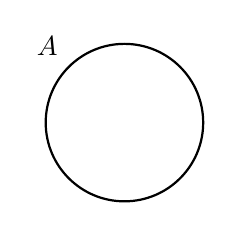
\begin{tikzpicture}[thick]
% Circle with label
\node[draw,
    circle,
    minimum size =2cm,
    label=135:$A$] (circle1) at (0,0){};
\end{tikzpicture} \]

Given two sets $A,B$ there are now four possibilities for all objects in the universe:
\begin{enumerate}
\item outside both $A$ and $B$;
\item inside $A$, but not inside $B$;
\item inside $B$, but not inside $A$;
\item inside both $A$ and $B$.
\end{enumerate}
We correspondingly divide the paper into four regions:
\[ 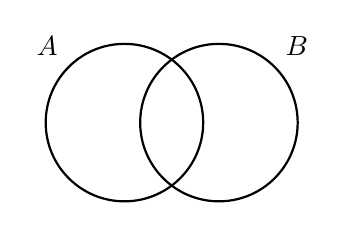
\begin{tikzpicture}[thick]
% Set A
\node [draw,
    circle,
    minimum size =2cm,
    label={135:$A$}] (A) at (0,0){};
% Set B
\node [draw,
    circle,
    minimum size =2cm,
    label={45:$B$}] (B) at (1.2,0){};
\end{tikzpicture} \]

For three sets $A,B,C$ the picture becomes:
\[ 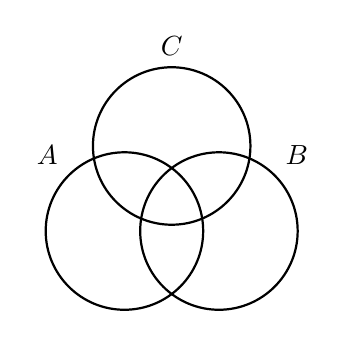
\begin{tikzpicture}[thick]
% Set A
\node[draw,circle,minimum size =2cm,label={135:$A$}] (A) at (0,0) {};

% Set B
\node[draw,circle,minimum size =2cm,label={45:$B$}] (B) at (1.2,0) {};

% Set C
\node[draw,circle,minimum size =2cm,label=$C$] (C) at (0.6,1.08) {};
\end{tikzpicture} \]

If we want to show that one set is a subset of another set, e.g. $B\subset A$, then we can represent this as follows:
\[ 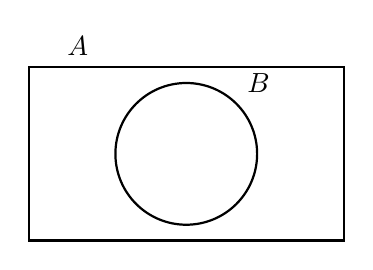
\begin{tikzpicture}[thick]
% Set A
\node [draw,
    rectangle,
    minimum width =4cm,
	minimum height = 2.2cm,
    label={135:$A$}] (A) at (0,0){};
% Set B
\node [draw,
    circle,
    minimum size =1.8cm,
    label={45:$B$}] (B) at (0,0){};
\end{tikzpicture} \]

Expressions talking about sets can be expressed by shading regions of Venn diagrams. For example $A\cup B$:
\[ 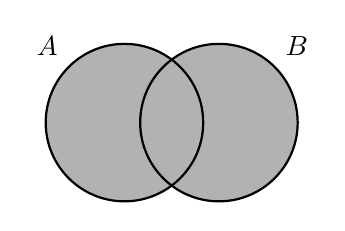
\begin{tikzpicture}[thick,
    set/.style = {circle,
        minimum size = 2cm,
        fill=black!30}]

% Set A
\node[set,label={135:$A$}] (A) at (0,0) {};

% Set B
\node[set,label={45:$B$}] (B) at (1.2,0) {};

% Circles outline
\draw (0,0) circle(1cm);
\draw (1.2,0) circle(1cm);
\end{tikzpicture} \]

\subsection{Operations on sets}
\subsubsection{Intersection}
\begin{definition}
The \udef{intersection} of an object $\mathcal{E}$ is a set $\bigcap \mathcal{E}$ defined by
\[ \bigcap \mathcal{E} \defeq \left\{ x\in \bigcup\mathcal{E} \;|\; \forall X\in \mathcal{E}: x\in X \right\}. \]
\end{definition}
As before, for the union, we define
\[ A\cap B \defeq \bigcap \{A,B\}. \]

The intersection $A\cap B$ can be represented in a Venn diagram as follows:
\[ 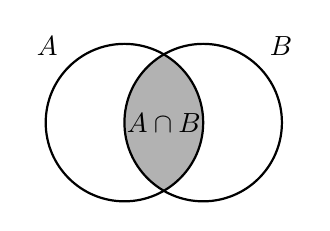
\begin{tikzpicture}[thick,
    set/.style = {circle,
        minimum size = 2cm}]

% Set A
\node[set,label={135:$A$}] (A) at (0,0) {};

% Set B
\node[set,label={45:$B$}] (B) at (1,0) {};

% Intersection
\begin{scope}
    \clip (0,0) circle(1cm);
    \clip (1,0) circle(1cm);
    \fill[black!30](0,0) circle(1cm);
\end{scope}

% Circles outline
\draw (0,0) circle(1cm);
\draw (1,0) circle(1cm);

% Set intersection label
\node at (0.5,0) {$A\cap B$};
\end{tikzpicture} \]

\subsubsection{Difference}
\begin{definition}
Given two objects $A,B$, we define the \udef{difference} as
\[A\setminus B \defeq \setbuilder{ x\in A}{x\notin B}. \]
\end{definition}
The difference $A\setminus B$ can be represented in a Venn diagram as follows:
\[ 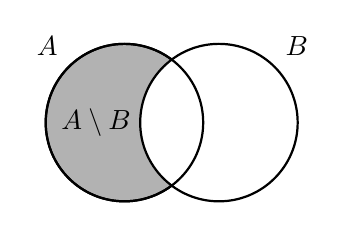
\begin{tikzpicture}[thick,
    set/.style = {circle,
        minimum size = 2cm}]

% Set A
\node[set,draw,fill=black!30,label={135:$A$}] (A) at (0,0) {};

% Set B
\node[set,draw,fill=white,label={45:$B$}] (B) at (1.2,0) {};

% Circles outline
\draw (0,0) circle(1cm);

% Set label
\node at (-0.36,0) {$A\setminus B$};
\end{tikzpicture} \]

\begin{proposition}[De Morgan's laws]
Let $A,B,C$ be sets. Then
\begin{align*}
C\setminus (A\cap B) &= (C\setminus A)\cup(C\setminus B) \\
C\setminus (A\cup B) &= (C\setminus A)\cap(C\setminus B)
\end{align*}
This can be extended to arbitrary families of sets:
\begin{align*}
C\setminus\left(\bigcup \mathcal{E}\right) &= \bigcap\setbuilder{C\setminus A}{A\in\mathcal{E}} \\
C\setminus\left(\bigcap \mathcal{E}\right) &= \bigcup\setbuilder{C\setminus A}{A\in\mathcal{E}}
\end{align*}
where $\mathcal{E}$ is a family of sets.
\end{proposition}
\begin{lemma}
Let $\mathcal{E}$ be a family of sets and $A$ a set. Then
\[ \bigcup \mathcal{E} \setminus A = \bigcup\setbuilder{X\setminus A}{X\in\mathcal{E}} \qquad\text{and}\qquad \bigcap \mathcal{E} \setminus A = \bigcap\setbuilder{X\setminus A}{X\in\mathcal{E}}. \]
\end{lemma}

\begin{lemma} \label{lemma:differenceProperties}
Let $A,B,C$ be sets. Then
\begin{enumerate}
\item $(A\setminus B)\setminus C = A\setminus (B\cup C)$;
\item $A\setminus (B\setminus C) = (A\setminus B) \cup (A\cap C)$;
\end{enumerate}
and
\begin{enumerate} \setcounter{enumi}{2}
\item $(A\setminus B)\cap C = (A\cap C)\setminus B = A\cap (C\setminus B)$;
\item $(A\setminus B)\cup C = (A\cup C)\setminus (B\setminus C)$;
\end{enumerate}
and
\begin{enumerate} \setcounter{enumi}{4}
\item $A\setminus A = \emptyset$;
\item $\emptyset\setminus A = \emptyset$;
\item $A\setminus \emptyset = A$.
\end{enumerate}
\end{lemma}

\subsubsection{Symmetric difference}
\begin{definition}
We define the \udef{symmetric difference} of two sets $A,B$ as
\[ A \symdiff B \defeq (A\setminus B)\cup(B\setminus A). \]
This is equivalent to $A\symdiff B = \setbuilder{x\in A\cup B}{(x\in A)\oplus (x\in B)}$.
\end{definition}

The symmetric difference $A\symdiff B$ can be represented in a Venn diagram as follows:
\[ 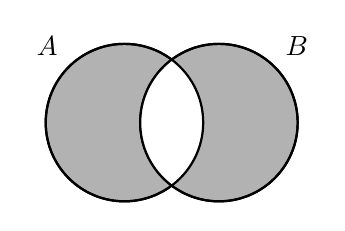
\begin{tikzpicture}[thick,
    set/.style = {circle,
        minimum size = 2cm}]

% Set A
\node[set,draw,fill=black!30,label={135:$A$}] (A) at (0,0) {};

% Set B
\node[set,draw,fill=black!30,label={45:$B$}] (B) at (1.2,0) {};

\begin{scope}
    \clip (0,0) circle(1cm);
    \clip (1.2,0) circle(1cm);
    \fill[white](0,0) circle(1cm);
\end{scope}

% Circles outline
\draw (0,0) circle(1cm);
\draw (1.2,0) circle(1cm);
\end{tikzpicture} \]

\begin{lemma}
Let $A,B,C$ be sets. Then
\begin{align*}
A\symdiff \emptyset &= A \\
A\symdiff B = \emptyset &\iff A = B
\end{align*}
and
\begin{align*}
A \symdiff B &= B \symdiff A \\
(A \symdiff B) \symdiff C &= A \symdiff (B \symdiff C) \\
A \symdiff C &= (A \symdiff B)\symdiff(B \symdiff C).
\end{align*}
\end{lemma}

\subsection{Identities and equivalences}
\subsubsection{Identities involving families of sets}
\begin{lemma}
Let $\mathcal{F}, \mathcal{G}$ be families of sets such that $\mathcal{F}\subseteq \mathcal{G}$. Then
\begin{enumerate}
\item $\bigcup \mathcal{F} \subseteq \bigcup \mathcal{G}$;
\item $\bigcap \mathcal{F} \supseteq \bigcup \mathcal{G}$.
\end{enumerate}
\end{lemma}

\subsubsection{Set operations and statements characterised}
\begin{lemma}
Let $A,B$ be sets. Then
\begin{enumerate}
\item $\begin{aligned}[t]
A\cap B &= A\setminus (A\setminus B) \\
&= B\setminus (A\symdiff B) \\
&= A\symdiff (A\setminus B);
\end{aligned}$
\item $\begin{aligned}[t]
A\cup B &= (A\symdiff B)\cup A \\
&= (A\symdiff B)\symdiff(A\cap B) \\
&= (A\setminus B)\cup B;
\end{aligned}$
\item $\begin{aligned}[t]
A\symdiff B &= (A\cup B)\setminus (A\cap B) \\
&= (A\symdiff C)\symdiff(C\symdiff B)
\end{aligned}$

for any set $C$;
\item $\begin{aligned}[t]
A\setminus B &= A\setminus (A\cap B) \\
&= A\cap(A\symdiff B) \\
&= (A\cup B)\symdiff B \\
&= A\symdiff (A\cap B);
\end{aligned}$
\end{enumerate}
\end{lemma}

\begin{lemma}
Let $A$ be a set. Then the following are equivalent:
\begin{enumerate}
\item $A$ is empty;
\item $A\cup B\subseteq B$ for every set $B$;
\item $A\subseteq B$ for every set $B$;
\item $A\subseteq (B\setminus A)$ for some set $B$;
\item $A\subseteq (B\setminus A)$ for every set $B$;
\item $\emptyset \setminus A= A$.
\end{enumerate}
\end{lemma}

\begin{lemma}
Let $A,B$ be sets. Then following are equivalent:
\begin{enumerate}
\item $A\subseteq B$;
\item $A\cap B = A$;
\item $A\cup B = B$;
\item $A\symdiff B = B\setminus A$;
\item $A\symdiff B \subseteq B\setminus A$
\item $A\setminus B = \emptyset$.
\end{enumerate}
For any universe set $\Omega$ such that $A,B\subset \Omega$ the above is also equivalent to
\begin{enumerate}\setcounter{enumi}{4}
\item $\Omega\setminus B \subseteq \Omega\setminus A$;
\item $(\Omega\cap A)\setminus B = \emptyset$;
\item $(\Omega\setminus A)\cup B = \Omega$.
\end{enumerate}
\end{lemma}
\begin{corollary}
Let $A,B$ be sets. Then following are equivalent:
\begin{enumerate}
\item $A=B$;
\item $A\symdiff B = \emptyset$;
\item $A\setminus B = B\setminus A$.
\end{enumerate}
\end{corollary}

\subsubsection{Distributivity}
TODO: tables complete / correct??
\begin{lemma}
We say $*$ left distributes over $\bullet$ if
\[ A*(B\bullet C) = (A*B)\bullet (A*C) \qquad\text{for all sets $A,B,C$.} \]
This gives the table
\[ \begin{array}{c | c c c c c}
\text{\diagbox{$*$}{$\bullet$}} & \cup & \cap & \symdiff & \setminus & \times \\ \hline
\cup & \checkmark & \checkmark &  & & \\
\cap & \checkmark & \checkmark & \checkmark & \checkmark & \\
\symdiff &  &  &  & & \\
\setminus &  &  &  & & \\
\times & \checkmark & \checkmark &  & \checkmark &
\end{array} \]
\end{lemma}

\begin{lemma}
We say $*$ right distributes over $\bullet$ if
\[ (A\bullet B)*C = (A*C)\bullet (B*C) \qquad\text{for all sets $A,B,C$.} \]
This gives the table
\[ \begin{array}{c | c c c c c}
\text{\diagbox{$*$}{$\bullet$}} & \cup & \cap & \symdiff & \setminus & \times \\ \hline
\cup & \checkmark & \checkmark &  & & \\
\cap & \checkmark & \checkmark & \checkmark & \checkmark & \\
\symdiff &  &  &  & & \\
\setminus & \checkmark & \checkmark & \checkmark & \checkmark & \\
\times & \checkmark & \checkmark &  & \checkmark &
\end{array} \]
\end{lemma}

For more identities, see \url{https://en.wikipedia.org/wiki/List_of_set_identities_and_relations}.

\section{Classes}
Not every unary definite condition determines a set (e.g. $P(x) = x\notin x$ does not by Russell's paradox). We do, however, say there is a \udef{class} associated to the unary condition. We write
\[ C = \{ x\;|\; P(x) \} \]
and say $x$ is an element of the class $C$, or $x$ is in the class $C$ if $x$ is an object (in the universe $\mathcal{W}$) and $P(x)$ is true.

In essence we are just rephrasing the logical content of $P$ is a language reminiscent of collections. In this vein we also define inclusion among classes $C,D$ as
\[ C\subseteq D \defequiv \forall x: x\in C \implies x\in D. \]

A unary condition $P$ is \udef{coextensive} with a set $A$ if the objects which satisfy it are exactly the members of $A$. Not every $P$ is coextensive with a set and $P$ is coextensive with at most one set.

\chapter{Relations and functions}
Based on the definitions and axioms posited so far we can start to construct the objects that form the focus of mathematical study.
\section{Tuples}
Tuples represent a finite ordered collection of objects. They are usually written using parentheses.
\begin{example}
\begin{itemize}
\item The tuple $(a,b)$ contains $a$ as its first element and $b$ as its second element.
\item The tuple $(1,2,3)$ contains $1$ as its first element, $2$ as its second and $3$ as its third.
\end{itemize}
\end{example}
There are multiple set-theoretical implementations of tuples.

Using our notion of tuple, we can construct the \udef{Cartesian product} of two sets $A,B$:
\[ A\times B \defeq \left\{ (a,b) \;|\; a\in A\land b\in B \right\}. \]

\begin{lemma}
Let $A$ be a set. Then
\[ A\times \emptyset = \emptyset\times A = \emptyset. \]
\end{lemma}

\begin{definition}
An \udef{(ordered) pair operation} satisfies:
\begin{itemize}
\item $(a,b) = (x,y) \iff (a=x)\land (b=y)$;
\item the Cartesian product $A\times B = \left\{ (a,b) \;|\; a\in A\land b\in B \right\}$ is a set.
\end{itemize}
\end{definition}
Note that for the second condition it is enough to check that $A\times B$ is a subset of some set $S$. Then, by separation, $A\times B$ is the set
\[ A\times B = \{ x\in S\;|\; \exists a\in A:\exists b\in B: x = (a,b) \}. \]


\begin{definition}
Let $p = (a,b)$ be a pair, we use $\pi_1(p)$ to denote the first element of $p$ and $\pi_2(p)$ to denote the second element:
\[ p = (\pi_1(p),\pi_2(p)). \]
We can convert a pair to a set:
\[ \operatorname{set}((a,b)) = \{a,b\}. \]
\end{definition}
\subsection{Defining pairs}
\subsubsection{The Kuratowski pair}
\begin{definition}
The \udef{Kuratowski pair} is defined as
\[ (a,b) \defeq \{\{a\}, \{a,b\}\} \]
\end{definition}
Note that when $a=b$ we have
\[ (a,a) = \{\{a\},\{a,a\}\} = \{\{a\},\{a\}\} = \{\{a\}\}. \]
\begin{lemma}
Given a Kuratowski pair $p = (a,b)$, we can extract the first element $\pi_1(p)$ and the second element $\pi_2(p)$ as follows:
\begin{align*}
\pi_1(p) &= \bigcup\bigcap p; \\
\pi_2(p) &= \bigcup\left\{ x\in\bigcup p\;|\; \left[\bigcup p \neq \bigcap p\right] \implies \left[ x\notin \bigcap p \right] \right\}.
\end{align*}
The Kuratowski pair can be converted to a set by
\[ \operatorname{set}(p) = \bigcup p. \]
\end{lemma}
The construction ``$\left[\bigcup p \neq \bigcap p\right] \implies$'' in the formula for $\pi_2(p)$ is there so that it still works in case the first and second elements are the same.
\begin{proposition}
The Kuratowski pair is adequate, in that is satisfies
\[ (a,b) = (x,y) \iff (a=x)\land (b=y) \]
and the Cartesian product is a set.
\end{proposition}
\begin{proof}
If $(a=x)\land (b=y)$, then
\[ \{\{a\},\{a,b\}\} = \{\{x\},\{x,y\}\} \]
and thus $(a,b) = (x,y)$.

Now assume $(a,b) = (x,y)$. We consider two cases: $a=b$ and $a\neq b$.
\begin{itemize}[leftmargin=2cm]
\item[$\boxed{a=b}$] Then $(a,b) = \{\{a\},\{a,a\}\} = \{\{a\}\} = (x,y)$ and thus $\{x\} = \{x,y\} = \{a\}$ by extensionality. This implies $a=x=y$ and thus $(a=x)\land (b=y)$.
\item[$\boxed{a\neq b}$] Now $(a,b) = (x,y)$ implies
\[ \{\{a\},\{a,b\}\} = \{\{x\},\{x,y\}\}. \]
By extensionality, either $\{x\} = \{a\}$ or $\{x\} = \{a,b\}$. In the second option $a=x=b$ and thus $a=b$ which is a contradiction. So $x=a$.

Again by extensionality, either $\{x,y\} = \{a\}$ or $\{x,y\} = \{a,b\}$. In the first case $(x,y)$ would be a singleton and then by equality so would $(a,b)$, yielding a contradiction. Thus $\{x,y\} = \{a,b\}$. We know $a=x$ and $b\neq a$, so by extensionality $b=y$.
\end{itemize}
To prove the Cartesian product $A\times B$ is a set, notice that
\begin{align*}
a\in A, b\in B &\implies \{a\},\{a,b\}\subseteq A\cup B \implies \{a\},\{a,b\}\in \powerset(A\cup B)\\
&\implies \{\{a\},\{a,b\}\}\subseteq \powerset(A\cup B) \implies \{\{a\},\{a,b\}\}\in \powerset(\powerset(A\cup B)) \\
&\implies (a,b) \in \powerset(\powerset(A\cup B)).
\end{align*}
and $\powerset(\powerset(A\cup B))$ is a set. So
\[ A\times B = \{ x\in \powerset(\powerset(A\cup B))\;|\; \exists a\in A:\exists b\in B: x = (a,b) \} \]
is a set.
\end{proof}
\subsubsection{The short variant}
We can also define a pair as
\[ (a,b) \defeq \{a,\{a,b\}\} \]
The advantage of this short definition is fewer braces. Some disadvantages include:
\begin{enumerate}
\item If $a$ and $b$ have the same type, $a$ and $\{a,b\}$ do not have the same type.
\item In order to prove adequacy, we need a new axiom, the axiom of regularity.
\end{enumerate}
\subsubsection{Using $0,1$}
Suppose we have decided on two special, distinct objects $0,1$. Then we can define
\[ (a,b) \defeq \{\{0,a\},\{1,b\}\}. \]
\begin{proposition}
This definition satisfies the requirements for a pair.
\end{proposition}
\begin{proof}
Assuming $(a=x)\land (b=y)$, it is clear that $(a,b)=(x,y)$ as sets by extensionality.

Now assume $(a,b)=(x,y)$. In this implementation a pair always has two elements as a set. The reasoning by extensionality is simple and only slightly more difficult if $a,b,x,y$ are equal to $0$ or $1$.

The Cartesian product is a subset of $\powerset(\powerset(A\cup B\cup \{0,1\}))$ and thus a set.
\end{proof}
\subsubsection{Wiener pair}
The Wiener definition of a pair is
\[ (a,b) \defeq \{\{\emptyset,\{a\}\},\{\{b\}\}\}. \]
\begin{proposition}
This definition satisfies the requirements for a pair.
\end{proposition}

\subsection{Tuples as nested pairs}
Once we have an implementation of a pair (i.e. $2$-tuple) of objects, the other tuples can then be readily constructed as follows:
\begin{enumerate}
\item The $0$-tuple is represented by the empty set $\emptyset$;
\item A $1$-tuple containing $a$ is represented by $(a,\emptyset)$;
\item An n-tuple, with $n > 1$, can be defined as an ordered pair of its first entry and an $(n − 1)$-tuple which contains the remaining entries:
\[ (a_1,a_2,a_3,\ldots,a_n) = (a_1, (a_2,a_3,\ldots, a_n)). \]
\end{enumerate}
For example:
\begin{align*}
(1,2,3) &= (1,(2,(3,\emptyset))) \\
(1,2,3,4) &= (1,(2,(3,(4,\emptyset)))).
\end{align*}

\subsection{Structured sets}
\begin{definition}
A \udef{structured set} is a pair $U = (A,S)$ where $A$ is a set and $S$ is an arbitrary object.
\begin{itemize}
\item $A$ is the \udef{field} or \udef{space} of $U$, written $\operatorname{Field}(U)$;
\item $S$ is the \udef{frame} of $U$.
\end{itemize}
If we write $x\in U$, we mean $x\in \operatorname{Field}(U)$.
\end{definition}

Often the frame $S$ is a $n$-tuple. In this case we may write the structured set as an $n+1$-tuple by concatenating the field and the frame. E.g. $(A,(S_1,S_2,S_3))$ becomes $(A,S_1,S_2,S_3)$.

\section{Relations}
\begin{definition}
Let $A,B$ be sets and $G$ any subset of the Cartesian product $A\times B$. A \udef{binary relation} $R$ on $(A, B)$ is a structured set $(G,(A,B))$. The \udef{graph} of the binary relation is the set $\graph(R) \defeq G$.
We write
\[ xRy \defequiv  (x,y)\in \graph(R). \]
Analogously we can define \udef{ternary relations} on $(A,B,C)$ as structured sets $(G,(A,B,C))$ where $G \subset A\times B\times C$. A similar definition can be made for $n$-ary relations.
\end{definition}

\subsection{Binary relations}
\begin{definition}
Let $R = (G,(A\times B))$ be a binary relation.
\begin{itemize}
\item $A$ is the \udef{domain} of the relation, denoted $\dom(R)$.
\item $B$ is the \udef{codomain} of the relation, denoted $\codom(R)$.
\end{itemize}
A binary relation is \udef{homogeneous} or an \udef{endorelation} if it has the same domain and codomain.
If we say $R$ is a relation on $A$, we mean it is an endorelation on $(A,A)$. 

A relation is \udef{heterogeneous} is the domain and codomain are different.
\end{definition}

\subsubsection{Related elements: image, preimage and polars}
\begin{definition}
Let $R$ be a binary relation. We say
\begin{itemize}
\item $x$ is \udef{related to} or \udef{comparable with} $y$ if either $xRy$ or $yRx$; we denote this $x\nparallel_R y$ or just $x\nparallel y$;
\item $x$ is \udef{unrelated to}, \udef{incomparable with} or \udef{parallel with} $y$ if neither $xRy$ nor $yRx$; we denote this $x\parallel_R y$ or just $x\parallel y$;
\item $x$ is \udef{left related} to $y$ if $xRy$;
\item $x$ is \udef{right related} to $y$ if $yRx$.
\end{itemize}
\end{definition}

\begin{definition}
Let $R$ be a relation on $(A, B)$.
\begin{itemize}
\item The \udef{image} of a subset $X\subset A$ under $R$ is the set
\[ XR \defeq \setbuilder{b\in B}{\exists x\in X: xRb}. \]
\item The \udef{preimage} of a subset $Y\subset B$ under $R$ is the set
\[ RY \defeq \setbuilder{a\in A}{\exists y\in Y: aRy}. \]
\end{itemize}
In particular for $X=A$ and $Y=B$:
\begin{enumerate}
\item The set $AR$ is the \udef{active codomain}, \udef{codomain of definition}, \udef{image} or \udef{range} of the relation, also denoted $\im(R)$.
\item The set $RB$ is the \udef{active domain}, \udef{domain of definition}, \udef{preimage} or \udef{prerange} of the relation.
\end{enumerate}
Replacing ``$\exists$'' by ``$\forall$'' in the previous definitions gives the definitions of the \udef{derivation operators} or \udef{polars}: TODO!
\begin{itemize}
\item The \udef{image} of a subset $X\subset A$ under $R$ is the set
\[ XR \defeq \setbuilder{b\in B}{\exists x\in X: xRb}. \]
\item The \udef{preimage} of a subset $Y\subset B$ under $R$ is the set
\[ RY \defeq \setbuilder{a\in A}{\exists y\in Y: aRy}. \]
\end{itemize}
\end{definition}

\begin{lemma} \label{lemma:imageRelation}
Let $R$ be a relation on $(A, B)$ and $X,Y\subset A$. Then
\begin{itemize}
\item $(X\cup Y)R = XR\cup YR$;
\item $(X\cap Y)R \subset XR\cap YR$;
\item $(X\setminus Y)R \supset XR\setminus YR$;
\item $(X\symdiff Y)R \supset XR\symdiff YR$.
\end{itemize}
\end{lemma}
\begin{lemma} \label{lemma:preimageRelation}
Let $R$ be a relation on $(A, B)$ and $X,Y\subset B$. Then
\begin{itemize}
\item $R(X\cup Y) = RX\cup RY$;
\item $R(X\cap Y) \subset RX\cap RY$;
\item $R(X\setminus Y) \supset RX\setminus RY$;
\item $R(X\symdiff Y) \supset RX\symdiff RY$.
\end{itemize}
\end{lemma}

\subsubsection{Properties of binary relations}
\begin{definition}
Let $R$ be a relation on $(A, B)$. We call $R$
\begin{itemize}
\item \udef{left-unique} or \udef{injective} if
\[ \forall x_1,x_2\in A\forall y\in B: x_1Ry \land x_2Ry \implies x_1=x_2; \]
\item \udef{right-unique} or \udef{functional} if
\[ \forall x\in A\forall y_1,y_2\in B: xRy_1 \land xRy_2 \implies y_1=y_2; \]
\item \udef{left-total} or \udef{serial} if
\[ \forall x\in A:\exists y\in B: xRy; \]
\item \udef{right-total} or \udef{surjective} or \udef{onto} if
\[ \forall y\in B:\exists x\in A: xRy; \]
\end{itemize}
\end{definition}
A binary relation may be
\begin{itemize}
\item \textbf{one-to-one}: injective and functional;
\item \textbf{one-to-many}: injective and not functional;
\item \textbf{many-to-one}: not injective and functional;
\item \textbf{many-to-many}: not injective and not functional.
\end{itemize}

\subsubsection{Properties of homogeneous relations}
\begin{definition}
Let $R$ be a homogeneous binary relation on a set $A$. We say
\begin{itemize}
\item $R$ is \udef{reflexive} if $\forall x\in A: xRx$;
\item $R$ is \udef{irreflexive} or \udef{anti-reflexive} if $\forall x\in A: \neg xRx$;
\item $R$ is \udef{quasi-reflexive} if every element that is related to some element is related to itself;
\item $R$ is \udef{left quasi-reflexive} if every element that is left related to some element is related to itself;
\item $R$ is \udef{right quasi-reflexive} if every element that is right related to some element is related to itself;
\item $R$ is \udef{coreflexive} if $xRy$ implies $x=y$.
\end{itemize}
We say
\begin{itemize}
\item $R$ is \udef{symmetric} if $\forall x,y\in A: xRy \implies yRx$;
\item $R$ is \udef{asymmetric} if $\forall x,y\in A: xRy \implies \neg yRx$;
\item $R$ is \udef{anti-symmetric} if $\forall x,y\in A: (xRy\land yRx) \implies x=y$.
\end{itemize}
We say
\begin{itemize}
\item $R$ is \udef{transitive} if $\forall x,y,z\in A: [xRy \land yRz] \implies xRz$;
\item $R$ is \udef{intransitive} if it is not transitive;
\item $R$ is \udef{anti-transitive} if it is never transitive:
\[ \forall x,y\in A: (xRy\land yRz) \implies \neq xRz.\]
\end{itemize}
We say
\begin{itemize}
\item $R$ is \udef{connex} (or \udef{connected} or \udef{complete}) if $\forall x,y\in A: xRy \lor yRx$;
\item $R$ is \udef{semi-connex} (or \udef{weakly connected} or \udef{total}) if $\forall x,y\in A: xRy \lor yRx \lor x=y$;
\item $R$ is \udef{trichotomous} if $\forall x,y\in A$, exactly one of $xRy, yRx$ or $x=y$ holds.
\end{itemize}
We say
\begin{itemize}
\item $R$ is \udef{(right) Euclidean} if $\forall x,y,z\in A: xRy \land xRz \implies yRz$;
\item $R$ is \udef{left Euclidean} if $\forall x,y,z\in A: yRx \land zRx \implies yRz$.
\end{itemize}
We say
\begin{itemize}
\item $R$ is \udef{dense} if $\forall x,y\in A: xRy \implies [\exists z\in A: xRz \land zRy]$.
\end{itemize}
\end{definition}

\begin{lemma}
\begin{enumerate}
\item An anti-transitive relation is always irreflexive.
\item An irreflexive and left- (or right-) unique relation is always anti-transitive.
\item An anti-transitive relation on a set of more than four elements elements is never connex.
\end{enumerate}
\end{lemma}

\subsubsection{Particular homogeneous relations}
\begin{definition}
Let $A,B$ be sets. We have the following relations:
\begin{itemize}
\item the \udef{empty relation} $E$ on $(A, B)$ has graph $\emptyset$;
\item the \udef{universal relation} $U_{A,B}$ on $(A, B)$ has graph $A\times B$;
\item the \udef{identity relation} $\id_A$ on $A$ has graph $\setbuilder{(x,y)\in A\times A}{x=y}$.
\end{itemize}
\end{definition}
The identity relation on $A$ is also known as the \udef{diagonal relation} on $A$.

TODO graph of dependencies.

\subsubsection{Operations on binary relations}
\paragraph{Converse relation}
\begin{definition}
Let $R$ be a relation on $(A, B)$. The \udef{converse} $R^\transp$ of $R$ is the relation on $B\times A$ with graph
\[ \graph(R^{\transp}) = \setbuilder{(y,x)}{(x,y)\in \graph(R)} \subset B\times A. \]
It is also known as the \udef{inverse}, \udef{transpose}, \udef{reciprocal}, \udef{opposite} or \udef{dual} of $R$.
\end{definition}

\begin{lemma}
Let $R$ be a relation on $(A, B)$. Then
\begin{enumerate}
\item $(R^\transp)^\transp = R$;
\item $\dom(R^\transp) = \codom(R)$ and $\codom(R^\transp) = \dom(R)$;
\item $R^\transp A = AR$ and $BR^\transp = RB$.
\end{enumerate}
\end{lemma}

\begin{lemma}
The following properties of binary endorelations are conserved under taking the converse:
\begin{enumerate}
\item all forms of reflexivity, except left and right quasi-reflexivity are swapped;
\item all forms of symmetry;
\item all forms of transitivity;
\item all forms of connexity and trichotomy;
\item density.
\end{enumerate}
Left and right Euclideanness are swapped.
\end{lemma}
\paragraph{Complementary relation}
\begin{definition}
Let $R$ be a binary relation on $(A, B)$. The \udef{complementary relation} $\overline{R}$ of $R$ is the relation on $(A, B)$ with graph
\[ \graph(\overline{R}) = \setbuilder{(x,y)}{\neg xRy}. \]
\end{definition}
\begin{lemma}
Let $R$ be a binary relation.
\begin{enumerate}
\item $\overline{\overline{R}} = R$;
\item $\overline{R^\transp} = \overline{R}^\transp$.
\end{enumerate}
\end{lemma}
\begin{lemma}
The following properties of binary endorelations are conserved under taking the converse:
\begin{enumerate}
\item symmetry;
\item asymmetry.
\end{enumerate}
The following properties are swapped:
\begin{enumerate}
\item reflexivity $\leftrightarrow$ irreflexivity.
\end{enumerate}
\end{lemma}
\paragraph{Composition of relations}
\begin{definition}
Let $R$ be a relation on $(A, B)$ and $S$ a relation on $(B, C)$. Then the \udef{composition} of $R$ and $S$ is a new relation $R;S$ on $(A, C)$ with graph
\[ \graph(R;S) = \setbuilder{(x,z)\in A\times C}{\exists y\in B: xRy \land ySz}. \]
If $R$ and $S$ are relations such that the codomain of one is the domain of the other, they are called \udef{composable}.

If $R$ and $S$ are composable we also define the notation
\[ S\circ R \defeq R;S. \]
\end{definition}
\begin{lemma}
Let $R,S,T$ be composable relations.
\begin{enumerate}
\item The composition is associative: $R;(S;T) = (R;S);T$.
\item The converse of $R;S$ is
\[ (R;S)^\transp = S^\transp ; R^\transp. \]
\end{enumerate}
\end{lemma}

\begin{lemma}
Let $R$ be a relation on $(A, B)$ and $S$ a relation on $(B, C)$. Let $X\subset A$ and $Y\subset C$. Then
\begin{enumerate}
\item $X(R;S) = (XR)S$ and $X(S\circ R) = ((X)R)S$;
\item $(R;S)Y = R(SY)$ and $(S\circ R)Y = R(SY)$.
\end{enumerate}
\end{lemma}

\paragraph{Restrictions and extensions}
\begin{definition}
Let $R$ be a relation on $(A, B)$, $X\subseteq A$ and $Y \subseteq B$. The \udef{restriction} of $R$ to $(X,Y)$ is the relation $R|^Y_X$ on $(X,Y)$ with graph
\[ \graph(R|^Y_X) = \graph(R)\cap (X\times Y). \]
\begin{itemize}
\item If $Y = B$, then the restriction is called the \udef{left-restriction} of $R$ to $X$ and denoted $\left.R\right|_X$.
\item If $X = A$, then the restriction is called the \udef{right-restriction} of $R$ to $Y$ and denoted $\left.R\right|^Y$.
\end{itemize}
If $S$ is a restriction of $R$, then $R$ is called an \udef{extension} of $S$.
\end{definition}

\begin{lemma}
Let $R$ be a relation on $(A, B)$, $X_1,X_2\subseteq A$ and $Y_1,Y_2 \subseteq B$. Then
\[ \left.\left(R|_{X_1}^{Y_1}\right)\right|_{X_2}^{Y_2} = R|_{X_1\cap X_2}^{Y_1\cap Y_2}. \]
\end{lemma}

\begin{lemma} \label{lemma:relationPropertiesRestriction}
The following properties of binary endorelations are conserved under taking left- and right-restrictions to the same set:
\begin{enumerate}
\item all forms of reflexivity;
\item all forms of symmetry;
\item all forms of transitivity;
\item all forms of connexity and trichotomy;
\item Euclideanness.
\end{enumerate}
\end{lemma}
Basically only not density.

\subsubsection{Operations on homogeneous relations}
\paragraph{Closures}
\begin{definition}
Let $R$ be a homogeneous relation on a set $A$.
\begin{itemize}
\item The \udef{reflexive closure} of $R$ is the relation $R^=$ on $A$ with graph
\begin{align*}
\graph(R^=) &= \bigcap\setbuilder{\graph(R')}{\text{$R'$ extends $R$ and is reflexive}} \\
&= \setbuilder{(x,x)\in A\times A}{x\in A}\cup \graph(R).
\end{align*}
\item The \udef{reflexive reduction} of $R$ is the relation $R^{\neq}$ on $A$ with graph
\[ \graph{R^{\neq}} = \graph(R)\setminus \setbuilder{(x,x)\in A\times A}{x \in A}. \]
\item The \udef{transitive closure} of $R$ is the relation $R^{+}$ on $A$ with graph
\[ \graph(R^+) = \bigcap\setbuilder{\graph(R')}{\text{$R'$ extends $R$ and is transitive}}. \]
\item The \udef{symmetric closure} of $R$ is the relation $R^{\leftrightarrow}$ on $A$ with graph
\begin{align*}
\graph(R^\leftrightarrow) &= \bigcap\setbuilder{\graph(R')}{\text{$R'$ extends $R$ and is symmetric}} \\
&=  \graph(R)\cup \graph(R^\transp).
\end{align*}
\end{itemize}
\end{definition}

\begin{lemma}
Let $R$ be a homogeneous relation on a set $A$.
\begin{enumerate}
\item The reflexive closure $R^=$ is the smallest reflexive relation on $A$ that extends $R$.
\item The reflexive reduction $R^{\neq}$ is the largest irreflexive relation on $A$ that is a restriction of $R$.
\item The transitive closure $R^{+}$ is the smallest transitive relation on $A$ that extends $R$.
\item The symmetric closure $R^{\leftrightarrow}$ is the smallest symmetric relation on $A$ that extends $R$.
\end{enumerate}
\end{lemma}

\begin{lemma}
The closures (and reduction) are monotone: if $R$ extends $S$, then $R^a$ extends $S^a$ for all $a,b\in\{=,+,\leftrightarrow,\neq\}$.
\end{lemma}

\begin{lemma}
Let $R$ be a homogeneous relation over a set $A$. Then all closures commute, i.e.
\[ R^a = R^b \qquad \forall a,b\in\{=,+,\leftrightarrow\}. \]
\end{lemma}
\begin{proof}
Only the equations involving $R^+$ are non-trivial. For example take $(R^\leftrightarrow)^+ = (R^+)^\leftrightarrow$. Now $(R^+)^\leftrightarrow$ is transitive, because transitivity is preserved under taking the symmetric closure, and contains $R^\leftrightarrow$, so $(R^\leftrightarrow)^+$ is extended by $(R^+)^\leftrightarrow$.

Conversely, take an $x\in (R^+)^\leftrightarrow$. Then either $x\in R^+$ or $x\in (R^\transp)^+$ and both $R^+\subseteq (R^\leftrightarrow)^+$ and $(R^\transp)^+\subseteq (R^\leftrightarrow)^+$. So $(R^+)^\leftrightarrow$ is extended by $(R^\leftrightarrow)^+$
\end{proof}

\begin{lemma}
Let $R$ be a homogeneous relation over a set $A$.
\begin{enumerate}
\item The reflexive transitive closure $R^*$ is the smallest preorder containing $R$.
\item The reflexive transitive symmetric closure $R^\equiv$ is the smallest equivalence relation containing $R$.
\end{enumerate}
\end{lemma}

\paragraph{Direct product}
TODO: extend: heterogeneous relations + direct product of two different relations.
\begin{definition}
Let $R$ be a homogeneous relation over a set $A$. We can turn $R$ into a relation over $(A, A)$ as follows:
\[ (a,b)R(c,d) \iff aRc \land bRd. \]
\end{definition}
\begin{lemma} \label{lemma:relationPropertiesDirectProduct}
The following properties of binary endorelations are conserved under taking the direct product:
\begin{enumerate}
\item all forms of reflexivity;
\item all forms of symmetry;
\item all forms of transitivity;
\item left and right Euclideanness;
\item density.
\end{enumerate}
The following properties are not necessarily conserved:
\begin{enumerate}
\item connexity;
\item semi-connexity;
\item trichotomy.
\end{enumerate}
\end{lemma}

\subsubsection{Some lemmas}
\begin{lemma}
Let $R$ be a homogeneous relation on $A$. Then
\[ R \;\text{is connex} \iff U_A \subseteq R\cup R^\transp \iff \overline{R}\subseteq R^\transp \iff \overline{R}\; \text{is asymmetric}. \]
\[ R\; \text{is semiconnex} \iff \overline{I}_A \subseteq R\cup R^\transp \iff \overline{R}\subseteq R^\transp\cup I_A \iff \overline{R}\; \text{is anti-symmetric}. \]
\end{lemma}

\subsection{Equivalence relations}
\begin{definition}
An \udef{equivalence relation} is a binary relation that is reflexive, symmetric and transitive.
\end{definition}
\begin{definition}
Let $\sim$ be an equivalence relation on $A$. Let $x\in A$. The \udef{equivalence class} of $x$ is the set
\[ [x]_\sim \defeq \{ y\in A\;|\; x\sim y \}. \]
Then $x$ is called a \udef{representative} of this equivalence class.

The set of all equivalence classes is called the \udef{quotient set} of $A$ by $\sim$
\[ A/\sim \defeq \{ [x]_\sim \in \powerset(A) \;|\; x\in A \}. \]
\end{definition}
\begin{proposition}
Let $\sim$ be an equivalence relation on $A$. The quotient set of $A$ by $\sim$ defines a \udef{partition} of $A$:
\begin{enumerate}
\item Every equivalence class is non-empty (each equivalence class has a representative);
\item every element of $A$ is in an equivalence class, i.e.
\[ A = \bigcup (A/\sim); \]
\item any two equivalence classes are either disjoint or the same:
\[ \forall x,y\in A: \qquad[x]_\sim \cap [y]_\sim = \emptyset \quad \lor \quad [x]_\sim = [y]_\sim. \]
\end{enumerate}
Conversely, every partition defines an equivalence relation.
\end{proposition}

\section{Functions}
TODO: equiv for equality!

\begin{definition}
A \udef{function} is a binary relation that is functional and serial.
\end{definition}
If a relation $f$ on $(A, B)$ is a function, then for every $x\in A$, there is a unique $y\in B$ such that $xfy$. We write $f(x)$ or $fx$ to denote this unique element.

Conceptually we can rephrase this as saying that for each ``input'' in the domain $A$, the function $f$ produces a unique ``output'' in the codomain $B$.

\begin{note}
We write
\[f:A \to B: x\mapsto f(x) \]
to show $f$ is a function with domain $A$ and codomain $B$ that maps $x\in A$ to $f(x)\in B$. We say $f$ is a function from $A$ to $B$ or $f$ maps $A$ to $B$. The set of all functions from $A$ to $B$ is denoted $(A\to B)$.
\end{note}

Depending on the context, functions may also be called \udef{maps} or \udef{transformations}. These are synonyms with slightly different connotations.

\begin{lemma}
Let $f_1: A_1\to B_1$ and $f_2: A_2\to B_2$ be functions. Then $f_1$ and $f_2$ are the same functions \textup{if and only if}
\begin{enumerate}
\item $A_1 = A_2$ and $B_1 = B_2$;
\item $\forall x\in A_1: f_1(x) = f_2(x)$.
\end{enumerate}
\end{lemma}

\subsection{Injectivity, surjectivity and bijectivity}
\begin{definition}
The terms injective and surjective are commonly applied to functions. A function that is both injective and surjective is \udef{bijective}.
\end{definition}
In the context of functions the notions of injectivity and one-to-one coincide.
\begin{lemma}
Let $f:A\to B$ be a function. We say
\begin{itemize}
\item $f$ is injective, denoted $f: A\rightarrowtail B$, if
\[ \forall x_1,x_2\in A: f(x_1) = f(x_2) \implies x_1 = x_2; \]
\item $f$ is surjective, denoted $f: A\twoheadrightarrow B$, if
\[ \forall y\in B: \exists x\in A: f(x) = y; \]
\item $f$ is bijective, denoted $f: A\twoheadrightarrowtail B$, if
\[ \forall y\in B: \exists! x\in A: f(x) = y; \]
\end{itemize}
We also say $f$ is an injection, a surjection or a bijection if it is injective, surjective or bijective, respectively.

We will also sometimes write $A \leftrightarrow B$, instead of $A\twoheadrightarrowtail B$, to denote a bijection between $A$ and $B$.
\end{lemma}

\begin{lemma}
If $A\subseteq B$ sets, then there exists a canonical injection $\iota: A\to B$, the \udef{inclusion map}
\[ \iota: A\to B: a\mapsto a. \]
The inclusion map is often denoted $A\hookrightarrow B$.
\end{lemma}

\subsection{Constructing new functions from old}
Constructions defined for relations are in particular applicable to functions.
\subsubsection{Composition}
\begin{lemma}
The functions $f:A\to B$ and $g:B\to C$ are composable as relations and the relation
\[ f;g = g\circ f \]
is a function. In particular it has functional form
\[ g\circ f: A\to C: x\mapsto g(f(x)). \]
\end{lemma}
Because of the simplicity of $(g\circ f)(x) = g(f(x))$, the notation $\circ$ is almost exclusively used, when dealing with functions.

\begin{definition}
Let $f, g:A\to A$ be functions. We say $f$ and $g$ \udef{commute} if $f\circ g = g\circ f$.
\end{definition}

\subsubsection{Restriction and extension}
\begin{lemma}
Let $f: A\to B$ be a function and $S\subset A$. Then $f|_S$ is a function.
\end{lemma}
When talking about the restriction of a function, this left restriction is always the one that is meant. Right restrictions $f|^K$ are sometimes called \udef{corestrictions} and are in general not functions.

\begin{definition}
Let $A\subset B$ and $C$ be sets. Let $f: A\to C$ be a function. A function $\tilde{f}: B\to C$ such that $\tilde{f}|_A = f$ is called an \udef{extension} of $f$.
\end{definition}
Given a function, a different function with as codomain a superset of the original codomain, which is otherwise identical, is sometimes called a \udef{coextension} of the function.

When given a function prescription, we may need to verify the function is \emph{well-defined} in the sense that the prescription always gives an element in the codomain for every element in the domain.

\subsubsection{Inverses of functions}
All identity relations are functions.

\begin{definition}
Let $f:X\to Y$ be a function.
\begin{itemize}
\item A \udef{left inverse} (or \udef{retraction}) of $f$ is a function $g: Y\to X$ such that
\[ g\circ f = \id_X. \]
\item A \udef{right inverse} (or \udef{section}) of $f$ is a function $h: Y\to X$ such that
\[ f\circ h = \id_Y. \]
\item A \udef{(two-sided) inverse} of $f$ is a function that is both a left and a right inverse.
\end{itemize}
\end{definition}

\begin{lemma}
Let $f:X\to Y$ be a function. The following are equivalent:
\begin{enumerate}
\item $f$ has a left inverse $g$;
\item $f^\transp$ is a partial function from $X$ to $Y$; 
\item $f^\transp \leq g$;
\item $f$ is injective.
\end{enumerate}
\end{lemma}
There is also a result linking the existence of a right inverse and surjectivity, but this in general only holds assuming the axiom of choice. (TODO ref)

\begin{lemma} \label{lemma:leftRightInverse}
If $f$ has a left inverse $g$ and a right inverse $h$, then $g=h$.
\end{lemma}
\begin{proof}
By the simple calculation
\[ g = g\circ (f\circ h) = (g\circ f) \circ h = h. \]
\end{proof}
Thus the two-sided inverse of $f$ is unique and exists \textup{if and only if} $f$ has a left and a right inverse. The unique two-sided inverse is denoted $f^{-1}$.

\begin{lemma}
Let $f:X\to Y$ be a function. The following are equivalent:
\begin{enumerate} 
\item the inverse exists;
\item the inverse exists and $f^{-1} = f^\transp$;
\item $f^\transp$ is a function from $X$ to $Y$;
\item $f$ is a bijection;
\item $f^\transp$ is a bijective function from $X$ to $Y$.
\end{enumerate}
\end{lemma}

\begin{lemma} \label{lemma:commutationInverse}
Let $f, g:A\to A$ be commuting and bijective functions. Then $f^{-1}$ and $g^{-1}$ commute.
\end{lemma}
\begin{proof}
We calculate
\[ f^{-1}\circ g^{-1} = f^{-1}\circ g^{-1}\circ (f\circ g \circ g^{-1} \circ f^{-1}) = f^{-1}\circ g^{-1}\circ (g\circ f) \circ g^{-1} \circ f^{-1} = g^{-1} \circ f^{-1} \]
\end{proof}



\subsection{Sets associated to functions}
\subsubsection{Image and preimage}
As functions are relations they have images and preimages. Let $f:A\to B$ be a function. We write
\begin{itemize}
\item $f[X]$ for the image $Xf$;
\item $f^{-1}[X]$ for the preimage $fX$.
\end{itemize}
We can associate to $f$
\begin{itemize}
\item an \udef{image function} $\powerset(A) \to \powerset(B)$ that maps subsets of $A$ to their image under $f$;
\item a \udef{preimage function} $\powerset(B) \to \powerset(A)$ that maps subsets of $B$ to their preimage under $f$.
\end{itemize}

A \udef{constant function} is a function whose range is a singleton.

\begin{lemma}
Let $f:A\to B$ be a function. Then the active domain of $f$ is the whole domain of $f$, i.e. $f^{-1}[B] = A$.
\end{lemma}
For any subset $X\subseteq B$: $f[f^{-1}[X]]\subseteq X$.

Let $f:A\to B$ be a function and $X,Y\subseteq B$. Then by the general theory of relations (\ref{lemma:preimageRelation})
\begin{itemize}
\item $f^{-1}[X\cup Y] = f^{-1}[X]\cup f^{-1}[Y]$;
\item $f^{-1}[X\cap Y] \subset f^{-1}[X]\cap f^{-1}[Y]$;
\item $f^{-1}[X\setminus Y] \supset f^{-1}[X]\setminus f^{-1}[Y]$;
\item $f^{-1}[X\symdiff Y] \supset f^{-1}[X]\symdiff f^{-1}[Y]$.
\end{itemize}
For functions we additionally have the following:
\begin{lemma} \label{lemma:preimageProperties}
Let $f:A\to B$ be a function and $X,Y\subseteq B$. Then
\begin{itemize}
\item $f^{-1}[X\cap Y] = f^{-1}[X]\cap f^{-1}[Y]$;
\item $f^{-1}[X\setminus Y] = f^{-1}[X]\setminus f^{-1}[Y]$;
\item $f^{-1}[X\symdiff Y] = f^{-1}[X]\symdiff f^{-1}[Y]$.
\end{itemize}
\end{lemma}

Let $f:A\to B$ be a function and $X,Y\subseteq A$. Then by the general theory of relations (\ref{lemma:imageRelation})
\begin{itemize}
\item $f[X\cup Y] = f[X]\cup f[Y]$;
\item $f[X\cap Y] \subset f[X]\cap f[Y]$;
\item $f[X\setminus Y] \supset f[X]\setminus f[Y]$;
\item $f[X\symdiff Y] \supset f[X]\symdiff f[Y]$.
\end{itemize}
For \emph{injective} functions we additionally have the following:
\begin{lemma}
Let $f:A\to B$ be an injective function and $X,Y\subseteq A$. Then
\begin{itemize}
\item $f[X\cap Y] = f[X]\cap f[Y]$;
\item $f[X\setminus Y] = f[X]\setminus f[Y]$;
\item $f[X\symdiff Y] = f[X]\symdiff f[y]$.
\end{itemize}
In fact any of these equalities is equivalent to $f$ being injective.
\end{lemma}

\subsubsection{The kernel of a function}
\begin{definition}
Let $f:A\to B$ be a function. The \udef{kernel} of $f$ is
\[ \ker f \defeq \setbuilder{(x,y)\in A\times A}{f(x) = f(y)}. \]
\end{definition}

\begin{lemma}
Let $f:A\to B$ be a function. Then
\begin{enumerate}
\item the kernel of $f$ is an equivalence relation on $A$;
\item viewing $f$ as a binary relation
\[ \ker f = f;f^\transp = f^{\transp}\circ f. \]
\end{enumerate}
\end{lemma}

\begin{definition}
An equivalence class $[x]_{\ker f}$ is called a \udef{fibre} of $f$.
\end{definition}

\begin{proposition}
Let $f:A\to B$ be a function. We can associate to $f$
\begin{enumerate}
\item a surjective function $f': A\to f[A]: x\mapsto f(x)$;
\item an injective function $f'': A/(\ker f) \;\to B: [x]_{\ker f}\mapsto f(x)$;
\item a bijective function $f''': A/(\ker f) \;\to f[A]: [x]_{\ker f}\mapsto f(x)$.
\end{enumerate}
\end{proposition}
Whenever a function on a quotient set defines an image of an equivalence class using an element of said equivalence class, we need to verify this definition is \emph{well-defined}, i.e. it does not depend on the chosen element in the equivalence class. (In other words it is properly a function of the equivalence class, not of the elements of the equivalence classes.)
\begin{proof}
We show $f''$ is well-defined. Let $[x]_{\ker f}\in A/(\ker f)$ and let $x_1,x_2\in [x]_{\ker f}$. Then $f(x) = f(x_1) = f(x_2)$ and
\[ f''([x_1]_{\ker f}) = f(x_1) = f(x_2) = f''([x_2]_{\ker f}), \]
so $f''$ is well-defined.
\end{proof}

\subsection{Functions with multiple inputs}
We can easily give a function multiple inputs from multiple domains by first joining them into an $n$-tuple, i.e. considering the Cartesian product of the domains as the domain of the function.

\begin{example}
A function $f$ that takes an input in $A$ and one in $B$ to generate an output in $C$ can be written as
\[ f: A\times B \to C: (a,b)\mapsto f(a,b). \]
\end{example}
\subsubsection{Currying}
\begin{definition}
Given a function $f: A\times B \to C$, we can \udef{curry} it to obtain a new function
\[ h: A \to (B\to C): a\mapsto f(a,-) \]
where $f(a,-)$ is the function
\[ f(a,-): B \to C: b\mapsto f(a,b). \]
\end{definition}
\begin{lemma}
For given sets $A,B,C$ the act of currying defines a bijective function
\[ \operatorname{curry}: (A\times B \to C) \to (A \to (B\to C)). \]
\end{lemma}

\subsubsection{Partial application}
\begin{definition}
Let $f: A\times B \to C$ be a function. A \udef{partial application} $p$ of $f$ is an element of the image of the curried function:
\[ p\in \operatorname{curry}(f)[A]. \]
\end{definition}

\section{Partial functions}
\begin{definition}
A \udef{partial function} is a relation that is functional (but not necessarily serial). If we wish to emphasise a function is both functional and serial, we may call it a \udef{total function}.
\end{definition}
If $f\subset A\times B$ is a partial function, we write $A\not \to B$. The set of all partial functions from $A$ to $B$ is
\[ (A\not \to B) = \bigcup _{S\subseteq A}(S\to B). \]

For all $a\in A$ we write
\[ f(a)\downarrow \defequiv a\in\dom(f),\qquad f(a)\uparrow \defequiv a\notin\dom(f) \]
We can read $f(a)\downarrow$ as ``$f$ converges at $a$'' and $f(a)\uparrow$ as ``$f$ diverges at $a$''.

\section{Identical domain and codomain}
TODO after natural numbers?

Let $f: A\to A$ be a function with $\dom(f) = \codom(f)$. Then we can define $f^n$ as the $n$-fold composition of $f$:
\[ f^n \defeq \underbrace{f\circ f \circ \ldots \circ f}_{\text{$n$ times}}. \]

\subsection{Fixed points}
\begin{definition}
Let $f: A\to A$ be a function with $\dom(f) = \codom(f)$. Then $x\in A$ is called a \udef{fixed point} if $f(x) = x$. 
\end{definition}

\begin{lemma} \label{lemma:fixedPointsMultipleComposition}
If $x\in A$ is a fixed point of $f:A\to A$, then $x$ is a fixed point of $f^n$ for all $n\in \N$.
\end{lemma}


\section{Relation isomorphisms}
\begin{definition}
Let $(A_1, R_1)$ and $(A_2, R_2)$ be relational structures. A bijection $\phi:A_1 \twoheadrightarrowtail A_2$ such that
\[ \forall (s_1,t_1)\in R_1: (\phi(s_1),\phi(t_1))\in R_2 \qquad \text{and} \qquad \forall (s_2,t_2)\in R_2: (\phi^{-1}(s_2),\phi^{-1}(t_2))\in R_1, \]
is called a \udef{(relation) isomorphism}. If there exists a relation isomorphism $A_1 \twoheadrightarrowtail A_2$, then $(A_1, R_1)$ and $(A_2, R_2)$ are \udef{isomorphic}, denoted $A_1 \cong A_2$.
\end{definition}

\begin{lemma} \label{lemma:isomorphismEquivalence}
Let $(A_1, R_1)$, $(A_2, R_2)$ and $(A_3, R_3)$ be relational structures and $f:A_1 \twoheadrightarrowtail A_2$, $g:A_2 \twoheadrightarrowtail A_3$ isomorphisms. Then
\begin{enumerate}
\item $I_{A_1}: A_1 \to A_1: a\mapsto a$ is an isomorphism;
\item $f^{-1}: A_2\to A_1$ is an isomorphism;
\item $(g\circ f): A_1\to A_3$ is an isomorphism.
\end{enumerate}
\end{lemma}
Consequently, relation isomorphism would be an equivalence relation on all structured sets, except there is no set of all structured sets, by Russell's paradox. Relation isomorphism can be an equivalence relation on a (restricted) set of structured sets.

\begin{lemma}
Let $(A_1, R_1)$ and $(A_2, R_2)$ be isomorphic relational structures. Then $R_1$ has the same properties as $R_2$.
\end{lemma}
E.g.: reflexivity, symmetry, transitivity, being an equivalence relation etc.


\chapter{The natural numbers}
TODO = 1:n!
\begin{definition}
A \udef{system of natural numbers} or \udef{Peano system} is a structured set $(N,(0,S)) = (N,0,S)$ which satisfies
\begin{enumerate}
\item $N$ is a set containing $0$;
\item $S$ is an injective function on the set $N$;
\item for all $n\in N: S(n) \neq 0$;
\item the induction principle: $\forall X\subset N$
\[ [(0\in X) \land (\forall n\in N: n\in X \implies Sn \in X)] \implies X = N. \]
\end{enumerate}
We call $0$ the \udef{zero} and $S$ the \udef{successor function}. These axioms are the \udef{Peano axioms}. An object $n\in N$ is called a \udef{successor} if $\exists m\in N: n = S(m)$.
\end{definition}
The most involved axiom is the induction principle. Note that it is not formulated in first order logic. Thus the Peano axioms are not subject to the Löwenheim–Skolem theorem and we can obtain a uniqueness result (despite the fact that, as we will see, $N$ is infinite).

\begin{lemma} \label{lemma:successor}
Let $(N,0,S)$ be a Peano system. Then every element $n\neq 0$ is a successor and for each $n\in N: S(n) \neq n$.
\end{lemma}
\begin{proof}
We wish to prove that the set
\[ X = \{n\in N\;|\; (n=0)\lor(\exists m\in N: n = S(m))\} \]
equals $N$. It is obvious that both $0\in X$ and $\forall n\in N: n\in X \implies Sn \in X$, so we can apply the induction principle to obtain $X=N$. The second claim then follows by injectivity.
\end{proof}
\section{Recursion and induction}
\subsection{Recursion}
\begin{theorem}[Recursion theorem]
Assume $(N,0,S)$ is a Peano system, $E$ is some set, $a\in E$, and $h:E\to E$ is some function.

There is exactly one function $f: N\to E$ which satisfies
\[ \begin{cases}
f(0) = a, \\
f(Sn) = h(f(n)) & (n\in N).
\end{cases} \]
\end{theorem}
Functions defined using this theorem are said to be defined \udef{recursively}.\footnote{The terms ``recursion'' and ``induction'' are often used synonymously. We
will usually distinguish recursive definitions from inductive
proofs (using the induction principle).}
\begin{proof}
We consider the set $\mathcal{A}$ of ``approximations'' of the function $f$:
\begin{align*}
\mathcal{A} = \{ p: X\to E \;|\; &(X\subset N)\land \\
&(0\in X)\;\land \\
&[\forall n\in N: Sn\in X \implies (n\in X \land p(Sn) = h(p(n)))] \}.
\end{align*}
In words we may say that $X$ is a downwards closed subset of $N$ and $p$ satisfies the recursion conditions. Some examples of elements of $\mathcal{A}$ include
\begin{align*}
&\{(0,a)\} \\
&\{(0,a), (S0, h(a))\} \\
&\{(0,a), (S0, h(a)), (SS0, h(h(a)))\} \\
&\;\;\ldots
\end{align*}

Any function $f$ with domain $N$ satisfying the recursion conditions, as in the theorem must be an element of $\mathcal{A}$. Thus to prove the theorem we need to prove that $\mathcal{A}$ contains exactly one function with domain $N$.

We prove this using a lemma.
\begin{lemma*}
For all $p,q\in \mathcal{A}$ and $n\in N$,
\[ n\in \dom(p)\cap\dom(q) \implies p(n) = q(n). \]
\end{lemma*}
\begin{proof}[Proof of lemma] \renewcommand{\qedsymbol}{$\dashv$ (Lemma)}
We need to prove that the set of $n\in N$ for which this is true,
\[ Y = \{n\in N \;|\; \forall p,q\in\mathcal{A}:\left[ n\in \dom(p)\cap\dom(q) \implies p(n) = q(n) \right] \} \]
is exactly $N$. We prove this with the principle of induction.

Clearly $0\in Y$, because every $p\in\mathcal{A}$ satisfies $p(0) = a$. Now let $n\in Y$ and $p,q\in\mathcal{A}$ such that $Sn\in \dom(p)\cap\dom(q)$. Then
\[ p(Sn) = h(p(n)) = h(q(n)) = q(Sn) \]
so $Sn\in Y$. By the induction principle $Y = N$.
\end{proof}
The lemma immediately implies there is at most one suitable function $f$ with domain $N$. We show such a function exists. Indeed it is given by $f = \bigcup \mathcal{A}$. Using the lemma we see this must be a function. It is not difficult to see that $f\in \mathcal{A}$. We then just need to verify that $\dom(f) = N$. This is again an application of the induction principle: $0\in \dom(f)$ and if $n\in \dom(f)$, then there exists some $p\in\mathcal{A}$ with $n\in\dom(p)$ and we have
\[ q = p\cup \{(Sn, h(p(n)))\}\in \mathcal{A}, \]
so that $Sn\in\dom(q)\subseteq \dom(f)$.
\end{proof}
\begin{corollary}[Recursion with parameters]
Let $(N,0,S)$ be a Peano system, $Y,E$ sets and functions
\[ g: Y\to E,\qquad h:E\times Y\to E. \]

There is exactly one function $f: N\times Y\to E$ which satisfies
\[ \begin{cases}
f(0,y) = g(y), & (y\in Y) \\
f(Sn,y) = h(f(n,y),y) & (y\in Y, n\in N).
\end{cases} \]
\end{corollary}
\begin{proof}
For any $y\in Y$ we can apply the normal recursion theorem the obtain a function $f_y: N\to E$. Then set $f(n,y) = f_y(n)$.
\end{proof}
\begin{corollary}[Recursion with the argument as parameter]
Let $(N,0,S)$ be a Peano system, $E$ a set, $a\in E$ and $h: E\times N\to E$ a function.

There is exactly one function $f: N\to E$ which satisfies
\[ \begin{cases}
f(0) = a, \\
f(Sn) = h(f(n),n) & (n\in N).
\end{cases} \]
\end{corollary}
\begin{proof}
Consider the function $\phi: N \to N\times E$ which returns both the required result and the successor of its argument. As the argument is returned by the function, it can be used in the normal recursion theorem if we replace $E$ by $N\times E$. Then just define $f(n)$ to be the second component of $\phi(n)$.
\end{proof}
More version of recursion can be cooked up, such as
\begin{itemize}
\item \udef{complete recursion} where at each step of the recursion. $h$ is passed not just the latest function value, but the whole partial function created so far:
\[ h: (\N \not\to E)\to E. \]
\item recursion with both the argument as parameter and other parameters;
\item simultaneous recursion that defines two functions $f_1,f_2$ and the next step depends on the current step of both functions:
\[ f_1(Sn) = h_1(f_1(n),f_2(n)) \qquad \text{and}\qquad f_2(Sn) = h_2(f_1(n),f_2(n)). \]
\end{itemize}

\subsection{Induction}
\begin{lemma}[Mathematical induction]
We can prove a definite statement $P(n)$ holds for all $n\in \N$ by proving
\begin{enumerate}
\item the \udef{base case} $P(0)$; and
\item the \udef{induction step} $\forall k\in \N: P(k)\implies P(Sk)$.
\end{enumerate}
We call ``$\forall k\in \N: P(k)$'' the \udef{induction hypothesis}.
\end{lemma}
\begin{proof}
Consider the set
\[ X = \{ n\in \N\;|\; P(n) \}. \]
The statement $P(n)$ holds for all $n\in \N$ if $X=\N$. Using the base case we have $0\in X$ and using the induction step we have
\[ \forall k\in\N: k\in X \implies Sn\in X. \]
By induction we conclude $X=\N$ and thus $P(n)$ for all $n\in \N$.
\end{proof}
\begin{corollary}
We can prove a definite statement $P(n)$ holds for all $n\geq n_0$ by proving
\begin{enumerate}
\item the base case $P(n_0)$; and
\item the induction step $\forall k\geq n_0: P(k)\implies P(Sk)$.
\end{enumerate}
\end{corollary}

\begin{lemma}[Complete (strong) induction]
We can prove a definite statement $P(n)$ holds for all $n\in \N$ by proving
\begin{enumerate}
\item the base case $P(0)$; and
\item the \udef{strong induction step} $\forall k\in \N: [\forall j\leq k:  P(j)] \implies P(Sk)$.
\end{enumerate}
\end{lemma}
The definition of $\leq$ follows later.
\begin{proof}
A strong inductive proof (i.e. proving these two steps) is a normal inductive proof of
\[ Q(n) \defequiv \forall m\leq n: P(m) \]
for all $n$. Clearly $Q(n)$ implies $P(n)$.
\end{proof}
Conversely we can prove nothing new using strong induction: every strong inductive proof is in particular also a (weak) inductive one.

\section{Existence and uniqueness of the natural numbers}
\begin{theorem} \label{theorem:existenceUniquenessPeano}
There exists a Peano system $(N,0,S)$. For any two Peano systems $(N_1,0_1,S_1)$ and
$(N_2,0_2,S_2)$ there exists a unique bijection $\pi: N_1 \to N_2$ such that
\[ \begin{cases}
\pi(0_1) = 0_2, \\
\pi(S_1n) = S_2\pi(n) & (n\in N_1).
\end{cases} \]
\end{theorem}
Such a bijection is called an \udef{isomorphism} of Peano systems. The theorem says any two Peano systems are (uniquely) isomorphic. So all Peano systems are essentially the same. We denote the all in the same way: $(\N, 0, S)$.
\begin{proof}
We first prove existence and then uniqueness.
\begin{itemize}
\item[\textbf{Existence}] By the axiom of infinity we have the set $I$ with properties
\[ \emptyset\in I \qquad \text{and}\qquad \forall n\in I: \{n\}\in I. \]
We then define
\[ \mathcal{J} = \{ X\subseteq I\;|\;[\emptyset\in X] \land [\forall n\in X: \{n\} \in X] \} \]
Then we set
\[ \N = \bigcap \mathcal{J},\qquad 0 = \emptyset, \qquad S: \N\to\N: n\mapsto \{n\}. \]
Note that by constructing $\mathcal{J}$ and then taking the intersection, we have removed possible other elements of $I$ and are left with
\[ \N = \{ \emptyset, \{\emptyset\}, \{\{\emptyset\}\}, \{\{\{\emptyset\}\}\}, \ldots \}. \]

With these definitions verifying the Peano axioms is not hard. The induction principle follows from the intersection.
\item[\textbf{Uniqueness}] By the recursion theorem we can a unique function $\pi$ satisfying the identities. What remains the be shown is that $\pi$ is bijective.
\begin{itemize}
\item[Surjectivity] We need to show that $\pi[N_1] = N_2$. To that end we use the induction principle on $(N_2,0_2, S_2)$.
\begin{itemize}
\item Obviously $0_2\in \pi[N_1]$, since $0_2=\pi(0_1)$.
\item Let $m\in\pi[N_1]$. Then $\exists n\in N_1: m=\pi(n)$. Applying $S_2$ gives
\[ S_2m = S_2\pi(n) = \pi(S_1 n). \]
This implies $S_2m\in \pi[N_1]$.
\end{itemize}
The induction principle then gives $\pi[N_1] = N_2$.
\item[Injectivity] We verify that the set
\[ X = \{ n\in N_1\;|\; \forall m\in N_1: \pi(m)=\pi(n) \implies m=n \} \]
equals the set $N_1$. This is again done using the induction principle.
\begin{itemize}
\item Firstly, if $m\neq 0_1$, then $m=S_1m'$ for some $m'\in N_1$, by lemma \ref{lemma:successor}. This implies
\[ \pi(m) = \pi(S_1m') = S_2\pi(m') \neq 0_2 \]
and so $0_1\in X$.
\item We need to show that, if $n\in X$,
\[ \pi(m) = \pi(S_1n) \implies m = S_1n. \]
Assume the antecendent. By hypothesis $\pi(m) = \pi(S_1n) = S_2\pi(n) \neq 0_2$ and thus $m\neq 0_1$. Again by lemma \ref{lemma:successor} $\exists m'\in N_1: m = S_1m'$. So
\[ S_2\pi(n) = \pi(m) = \pi(S_1m') = S_2\pi(m') \]
implying $n=m'$ and thus $m=S_1m'=S_1n$.
\end{itemize}
The induction principle then gives $X=N_1$ and thus the surjectivity of $\pi$.
\end{itemize}
\end{itemize}
\end{proof}

\subsection{Zermelo ordinals}
The natural numbers constructed in the existence proof are called \udef{Zermelo ordinals}. They are defined by
\[ 0 = \emptyset \qquad \text{and} \qquad S(a) = \{a\}. \]
Then
\begin{align*}
0 &= \emptyset \\
1 &= \{0\} = \{\emptyset\} \\
2 &= \{1\} =  \{\{\emptyset\}\} \\
3 &= \{2\} = \{\{\{\emptyset\}\}\} \\
&\hdots
\end{align*}
\subsection{(Finite) Von Neumann ordinals}
The \udef{Von Neumann ordinals} are an alternate construction. They are defined by
\[ 0 = \emptyset \qquad \text{and} \qquad S(a) = a\cup\{a\}. \]
Then
\begin{align*}
0 &= \emptyset \\
1 &= 0\cup \{0\} = \{\emptyset\} \\
2 &= 1\cup \{1\} = \{0,1\} = \{\emptyset, \{\emptyset\}\} \\
3 &= 2\cup \{2\} = \{0,1,2\} = \{ \emptyset, \{\emptyset\}, \{\emptyset, \{\emptyset\}\} \} \\
&\hdots
\end{align*}
Unlike the Zermelo ordinals, the Von Neumann ordinals can be readily generalised to infinite ordinals (see later).
\section{Operations and relations on natural numbers}
We can use the recursion theorem to define addition and multiplication.
\begin{definition}
The \udef{addition function} $+:\N\times \N \to \N$ on the natural numbers is defined by the recursion (with parameter)
\[ \begin{cases}
+(0,n) = n \\
+(Sm, n) = S(m+n)
\end{cases}. \]
The \udef{multiplication function} $\cdot:\N\times \N \to \N$ on the natural numbers is defined by the recursion (with parameter)
\[ \begin{cases}
\cdot(0,n) = 0 \\
\cdot(Sm, n) = (m\cdot n)+n
\end{cases}. \]
We will usually write $m+n$ and $m\cdot n$ or $mn$ instead of $+(m,n)$ and $\cdot(m,n)$.
\end{definition}

\begin{proposition}
Addition has the following properties:
\begin{enumerate}
\item It is associative: $(k+n)+m = k+(n+m)$;
\item $0$ is a neutral element: $0+n = n$ and $n+0 = n$;
\item for all $m,n\in \N: Sm+n = m+Sn$;
\item it is commutative: $n+m = m+n$.
\end{enumerate}
\end{proposition}
\begin{proof}
All are proven by induction on $m$. The proofs of later claims make use of earlier ones.
\end{proof}
\begin{lemma}
For all $n\in \N$, the function $\N\to \N: s\mapsto n+s$ is 1-1, so
\[n+s = n+t \implies s=t.\]
\end{lemma}

\begin{definition}
The binary relation $\leq$ defined by
\[ n \leq m \defequiv \exists s\in \N: n+s = m \]
is called the ordering of the natural numbers.

We abbreviate $\neg(m\leq n)$ by $n < m$.
\end{definition}

\begin{lemma} \label{lemma:orderingN}
Let $\N$ be ordered by $\leq$. Then $\forall n\in\N$
\begin{enumerate}
\item $0\leq n$;
\item there is no $m$ such that $n<m<n+1$.
\end{enumerate}
\end{lemma}
TODO proof

\begin{proposition} \label{proposition:wellOrderingN}
The endorelation $\leq$ on the natural numbers has the following properties:
\begin{enumerate}
\item it is transitive;
\item it is reflexive;
\item it is anti-symmetric;
\item it is connex (i.e. any two numbers are comparable);
\item every non-empty subset $S$ of $\N$ contains an element $x\in S$ that is left related to all elements of $S$: $\forall y\in S: x\leq y$.
\end{enumerate}
These are exactly the properties of a well-ordering.
\end{proposition}
\begin{proof}
Take a non-empty set $S\subset \N$ and define the set
\[ L = \setbuilder{n\in\N}{\forall m\in S: n\leq m}. \]
We need to show that $L\cap S$ is non-empty. Assume, towards a contradiction, that $L\cap S = \emptyset$.
Now
\begin{itemize}
\item $0\in L$.
\item If $n\in L$, then $n+1\in L$. Indeed if $n+1 \notin L$, then there exists a $z\in S$ such that $n\leq z<n+1$. But by \ref{lemma:orderingN} this would mean that $z=n$ and $n\in L\cap S = \emptyset$.
\end{itemize}
By induction $L=\N$, so $S = L\cap S = \emptyset$. This is a contradiction.
\end{proof}


The element $x$ in the last property is called the least element or minimum of $S$. It is unique by anti-symmetry and denoted $\min(S)$.

Some subsets $S$ of $\N$ contain an element $x\in S$ that is right related to all elements of $S$: $\forall y\in S: y\leq x$. If it exists, it is called the greatest element or maximum of $S$. It is again unique by anti-symmetry and denoted $\max(S)$.

\subsection{Enumerating pairs}
It will turn out to be useful to have a bijection
\[ \rho: \N\times \N \to \N. \]
We give two examples, the first due to Gödel, the second due to Zermelo.
\begin{lemma} \label{lemma:pairEnumeration}
The functions
\[\rho_1 : \N\times\N \to \N: (m,n)\mapsto \frac{(m+n)(m+n+1)}{2}+m \]
and
\[ \rho_1 : \N\times\N \to \N: (m,n)\mapsto \begin{cases}
(m+1)^2-1 & (m=n) \\
n^2 + m & (m<n) \\
m^2+m+n & (m>n)
\end{cases} \]
are bijections.
\end{lemma}
TODO pictures!
\section{Sequences and strings}
TODO: lower!
\begin{definition}
A \udef{sequence} in a set $A$ is a function
\[ x:I\subseteq\N\to A. \]
The domain $I$ is called the \udef{index set}.

We usually write $x_i$ instead of $x(i)$ and we denote the function $x$ as $\seq{x_i}_{i\in I}$ (or $\seq{x_i}$ if the index is clear).
\end{definition}
The choice of the index set is irrelevant up to a bijection. Thus which theorems hold depends on the cardinality of the index set (see later).

\begin{definition}
Let $\seq{x_i}_{i\in I}$ be a sequence. Let $f:I\to J\subset \N$ be an order-preserving bijection. Then we call $\seq{x_{f(i)}}_{i\in I}$ a \udef{subsequence} of the sequence $\seq{x_i}_{i\in I}$.

A \udef{tail} of the sequence $\seq{x_i}_{i\in I}$ is a subsequence where $f$ is the identity restricted to a set of the form
\[ \setbuilder{j\in I}{j\geq n} \]
for some $n\in I$.
\end{definition}

\subsection{Finite sequences}
\begin{definition}
A \udef{finite sequence} or \udef{word} or \udef{string} in a set $A$ is a sequence whose domain is a finite set.
This $n$ is the \udef{length} of the sequence, denoted $\len(x)$. We write
\begin{align*}
A^{(n)} &\defeq ([0,n[\to A) \\
A^* &\defeq \bigcup\left\{ A^{(n)}\in \powerset(\N\times A) \;|\;n\in \N \right\}.
\end{align*}
We call $A^*$ the \udef{Kleene closure} of $A$.

Let $a_0,\ldots, a_{n-1}\in A$. Then we have the string
\[ \langle a_0,\ldots, a_{n-1}\rangle \defeq \{(0,a_0),\ldots, (n-1,a_{n-1})\} \in A^{(n)}. \]
\begin{itemize}
\item If $u,v\in A^*$ and $u\subseteq v$, then $u$ is an \udef{initial segment} of $v$, denoted $u \sqsubseteq v$.
\item Let $u\in A^{(n)}, v\in A^{(m)}$ be strings. The \udef{concatenation} of $u$ and $v$ is the string
\[ u\star v \defeq \langle u_0,\ldots, u_{n-1},v_0,\ldots, v_{m-1}\rangle \in A^{(n+m)}. \]
\end{itemize}
\end{definition}
Notice that we can view tuples as strings of length two (i.e. there is a bijection $A\times A \leftrightarrow A^{(2)}$ for all sets $A$). Similarly an $n$-tuple can be seen as a string of length $n$. So sometimes we write
\[ A^* = \bigcup^\infty_{n=0}A^n = A^{<\omega}\]
where $A^{<\omega}$ is just a notational equivalent.

Notice that if $n$ is viewed as a Von Neumann ordinal, $A^{(n)} = A^n$.

We can think of $A^*$ as a generalisation of $\N$, with $\langle\rangle$ instead of $0$ and appending operators
\[ S_a(u) = u\star \langle a\rangle \]
for all $a\in A$.
\begin{theorem}[String recursion theorem]
Let $A,E$ be sets, $a\in E$, and $h:E\times A\to E$ some function.

There is exactly one function $f: A^*\to E$ which satisfies
\[ \begin{cases}
f(\langle\rangle) = a, \\
f(u\star \langle x\rangle) = h(f(u), x) & (u\in A^*, x\in A).
\end{cases} \]
\end{theorem}
\begin{proof}
Define a function $\phi: \N \times A^*\to E$ recursively such that it satisfies
\begin{align*}
\phi(0,u) &= a \\
\phi(n+1,u) &= h(\phi(n,u), u(n))
\end{align*}
and set $f(u) = \phi(\len(u), u)$. Proving that $f$ satisfies the second equality and the uniqueness of $f$ goes by induction on $\len(u)$.
\end{proof}
Like before, a version of the theorem can also be stated for recursion with parameters.
\subsection{Functions on finite sequences}
Let $f: A^{(m)}\to A^{(n)}$. We write
\[ f_k(a) = f(a)(k) \]
to denote the $k^\text{th}$ component of $f(a)$.

\chapter{The algebra of sets}
\section{Indexing and indexed sets}
\begin{definition}
Let $I$ be an arbitrary index set, $A$ some set and let there be a surjective function $a: I\twoheadrightarrow A: i \mapsto a_i$.

Then we say $A$ is \udef{indexed by I} and we write $A = \{a_i\}_{i\in I}$. In this case we call $A$ an \udef{(indexed) family}.

In particular if $A\subseteq \powerset(X)$ for some set $X$, $A$ is an indexed family of sets.
\end{definition}
Notice we do not require the function $a$ to be injective and thus multiple indexed elements may be the same.

Sometimes the notation $(a_i)_{i\in I}$ is used, if $I$ is ordered, to emphasise the ordering of $\{a_i\}_{i\in I}$ by $I$.

\subsection{Union and intersection of indexed families of sets}
Let $\{A_i\}_{i\in I}$ be an indexed family of sets. Then we write
\begin{align*}
\bigcup_{i\in I} A_i &\defeq \bigcup A[I] \\
\bigcap_{i\in I} A_i &\defeq \bigcap A[I]
\end{align*}
If $I = [0,n[$, we write $\{A_i\}_{i=1}^{n} \defeq \{A_i\}_{i\in [0,n[}$,
\[ \bigcup_{i=1}^{n-1} A_i \defeq \bigcup_{i\in [0,n[} A_i \qquad \text{and} \qquad \bigcap_{i=1}^{n-1} A_i \defeq \bigcap_{i\in [0,n[} A_i \]
and if $I=\N$, we write $\{A_i\}_{i=1}^{n} \defeq \{A_i\}_{i\in \N}$,
\[ \bigcup_{i=1}^{\infty} A_i \defeq \bigcup_{i\in \N} A_i \qquad \text{and} \qquad \bigcap_{i=1}^{\infty} A_i \defeq \bigcap_{i\in \N} A_i. \]

\begin{lemma}
Let $A$ be a set and $\{B_i\}_{i\in I}$ an indexed family of sets. Then
\begin{align*}
A\times \bigcup_{i\in I} B_i &= \bigcup_{i\in I}A\times B_i; \\
A\times \bigcap_{i\in I} B_i &= \bigcap_{i\in I}A\times B_i.
\end{align*}
\end{lemma}

\subsubsection{Multiple indices}
If the index set $I$ is a Cartesian product $I=J\times K$, then we also write
\[ \bigcup_{(j,k)\in I} A_{j,k} = \bigcup_{\substack{j\in J \\ k\in K}} A_{j,k} \qquad\text{and}\qquad \bigcap_{(j,k)\in I} A_{j,k} = \bigcap_{\substack{j\in J \\ k\in K}} A_{j,k}. \]

If $\{A_{j,k}\}_{(j,k) \in J\times K}$ is such an indexed family of sets, then $\{A_{j,k'}\}_{j\in J}$ is an indexed family of sets for each $k\in K$by partial application of $k'$ to the second argument. This allows us to apply union and intersection pointwise: we define
\[ \bigcup_{j\in J}A_{j,k} \defeq \left(k'\mapsto \bigcup_{j\in J}A_{j,k'}\right) \qquad\text{and}\qquad \bigcap_{j\in J}A_{j,k} \defeq \left(k'\mapsto \bigcap_{j\in J}A_{j,k'}\right) \]
as well as something similar for the first argument.

\subsubsection{Associativity and commutativity}
\begin{lemma} \label{lemma:setAssociativityCommutativity}
Let $\{A_{j,k}\}_{(j,k) \in J\times K}$ be an indexed family of sets. Then
\begin{align*}
\bigcup_{j\in J}\left(\bigcup_{k\in K}A_{j,k}\right) &= \bigcup_{\substack{j\in J \\ k\in K}}A_{j,k} = \bigcup_{k\in K}\left(\bigcup_{j\in J}A_{j,k}\right) \qquad\text{and} \\
\bigcap_{j\in J}\left(\bigcap_{k\in K}A_{j,k}\right) &= \bigcap_{\substack{j\in J \\ k\in K}}A_{j,k} = \bigcap_{k\in K}\left(\bigcap_{j\in J}A_{j,k}\right).
\end{align*}
\end{lemma}
\begin{corollary}
Let $\{A_{i}\}_{i \in I}$ be an indexed family of sets and $B$ a set. Then
\[ \left(\bigcup_{i\in I}A_i\right)\cup B = \bigcup_{i\in I}(A_i\cup B) \qquad\text{and}\qquad \left(\bigcap_{i\in I}A_i\right)\cap B = \bigcap_{i\in I}(A_i\cap B). \]
\end{corollary}
\begin{proof}
Set $J\times K = I\times\{0,1\}$ and $A_{j,k} = \begin{cases}
A_j & (k=0) \\
B & \text{(else)}
\end{cases}$.
\end{proof}
\begin{corollary}
Let $\{A_{i}\}_{i \in I}$ and $\{B_{j}\}_{j \in J}$ be indexed families of sets. Then
\[ \left(\bigcup_{i\in I}A_i\right)\cup \left(\bigcup_{j\in J}B_j\right) = \bigcup_{\substack{i\in I\\j\in J}}(A_i\cup B_j) \qquad\text{and}\qquad \left(\bigcap_{i\in I}A_i\right)\cap \left(\bigcap_{j\in J}B_j\right) = \bigcap_{\substack{i\in I\\j\in J}}(A_i\cap B_j). \]
If both families are indexed by the same index set $I$, we may take the union/intersection over just $I$, not $I\times I$.
\end{corollary}

\subsubsection{Distributivity}
\begin{lemma} \label{lemma:setDistributivity}
Let $\{A_{i}\}_{i \in I}, \{B_{j}\}_{j \in J}$ be indexed families of sets and $C$ a set. Then
\[ \left(\bigcup_{i\in I}A_i\right)\cap B = \bigcup_{i\in I}(A_i\cap B) \qquad\text{and}\qquad \left(\bigcap_{i\in I}A_i\right)\cup B = \bigcap_{i\in I}(A_i\cup B). \]
Also
\[ \left(\bigcup_{i\in I}A_i\right)\cap \left(\bigcup_{j\in J}B_j\right) = \bigcup_{\substack{i\in I\\j\in J}}(A_i\cap B_j) \qquad\text{and}\qquad \left(\bigcap_{i\in I}A_i\right)\cup \left(\bigcap_{j\in J}B_j\right) = \bigcap_{\substack{i\in I\\j\in J}}(A_i\cup B_j). \]
\end{lemma}

\begin{lemma}
Let $\{A_{j,k}\}_{(j,k) \in J\times K}$ be an indexed family of sets. Then
\[ \bigcup_{j\in J}\left(\bigcap_{k\in K}A_{j,k}\right) \subseteq \bigcap_{k\in K}\left(\bigcup_{j\in J}A_{j,k}\right). \]
\end{lemma}
In general these two sets are not equal!


\subsection{Arbitrary Cartesian products}
\begin{definition}
Let $\{A_i\}_{i\in I}$ be an arbitrary indexed family of sets, then we define the \udef{Cartesian product} of $\{A_i\}_{i\in I}$ to be
\[ \prod_{i\in I}A_i \defeq \left\{ f\in \left(\left. I \to \bigcup_{i\in I}A_i \right) \; \right| \; \forall i\in I: f(i) \in A_i \right\}. \]
For each $j\in I$, the function
\[ \pi_j : \prod_{i\in I}A_i \to A_j: f\mapsto f(j) \]
is called the \udef{$j^\text{th}$ projection map}.
\end{definition}

\begin{definition}
A Cartesian product of an indexed family of sets $\{A_i\}_{i\in I}$ is called a \udef{Cartesian power} of $A$ if for all $i\in I$, $A_i$ is the same set $A$. This is denoted $A^I$.
\end{definition}
If $I = [0,n[$ for some $n\in \N$, we write $A^n = A^I$.

Note that
\[ A^I = \prod_{i\in I} A = (I\to A).  \]

\begin{lemma}
There exists a bijection $A_0\times A_1 \leftrightarrow \prod_{i\in\{0,1\}} A_i$.
\end{lemma}
\begin{proof}
The bijection is given by
\[ (a,b) \quad\leftrightarrow\quad \{(0,a),(1,b)\} \qquad \forall a\in A_0, b\in A_1. \]
\end{proof}

\subsubsection{Distributing over unions and intersections}
\begin{lemma}
Let $\{A_{i}\}_{i \in I}$ and $\{B_{j}\}_{j \in J}$ be indexed families of sets, indexed over the same index family $I$. Then
\[ \left(\prod_{i\in I}A_i\right)\cap\left(\prod_{i\in I}B_i\right) = \prod_{i\in I}(A_i\cap B_i) \qquad\text{but}\qquad \left(\prod_{i\in I}A_i\right)\cup\left(\prod_{i\in I}B_i\right) \subset \prod_{i\in I}(A_i\cup B_i). \]
\end{lemma}

\begin{lemma}
Let $\{A_{i,j}\}_{(i,j) \in I\times J}$ be an indexed family of sets. Then
\[ \bigcap_{i\in I}\left(\prod_{j\in J}A_{i,j}\right) = \prod_{j\in J}\left(\bigcap_{i\in I}A_{i,j}\right) \qquad\text{but}\qquad \bigcup_{i\in I}\left(\prod_{j\in J}A_{i,j}\right) \subset \prod_{j\in J}\left(\bigcup_{i\in I}A_{i,j}\right). \]
\end{lemma}

\subsection{Disjoint union}
\begin{definition}
The \udef{disjoint union} of a family of sets $\{A_i\}_{i\in I}$ is defined as
\[ \bigsqcup_{i\in I}A_i \defeq \bigcup_{i\in I}\{i\}\times A_i. \]
If $A,B$ are sets, then we define
\[ A\sqcup B \defeq (\{0\}\times A)\cup (\{1\}\times B). \]
\end{definition}

\begin{lemma}
Let $\{A_i\}_{i\in I}$ be a family of sets.
\[ \bigsqcup_{i\in I}A_i = \left\{ (i,a)\in I\times \bigcup_{i\in I}A_i \;|\; a\in A_i \right\} \]
\end{lemma}

\subsection{Images and preimages}
\begin{lemma}
Let $R \subseteq A\times B$ be a relation, $\{X_i\}_{i\in I}$ a family of subsets of $A$ and $\{Y_j\}_{j\in J}$ a familiy of subsets of $B$. Then
\begin{enumerate}
\item $R\left(\bigcup_{j\in J} Y_j\right) = \bigcup_{j\in J} RY_j$;
\item $R\left(\bigcap_{j\in J} Y_j\right) \subseteq \bigcap_{j\in J} RY_j$;
\item $\left(\bigcup_{i\in I} X_i\right)R = \bigcup_{i\in I} X_iR$;
\item $\left(\bigcap_{i\in I} X_i\right)R \subseteq \bigcap_{i\in I} X_iR$.
\end{enumerate}
also
\begin{enumerate} \setcounter{enumi}{4}
\item if $R$ is functional, then $R\left(\bigcap_{j\in J} Y_j\right) = \bigcap_{j\in J} RY_j$;
\item if $R$ is injective, then $\left(\bigcap_{i\in I} X_i\right)R = \bigcap_{i\in I} X_iR$.
\end{enumerate}
\end{lemma}
In particular these result hold for functions.


\section{Families of sets}
\subsection{Universe sets and complementation}
\begin{definition}
Let $\mathcal{F}$ be a family of sets. A \udef{universe set} for this family is a set $U$ such that
\[ \forall A\in \mathcal{F}: A \subseteq U. \]
The \udef{complement} of a set $A\in\mathcal{F}$ w.r.t. $U$ is defined as
\[ A^c \defeq U\setminus A. \]

A \udef{unit} of $\mathcal{F}$ is a universe set contained in $\mathcal{F}$.
\end{definition}
\begin{lemma}
Let $\mathcal{F}$ be a family of sets. Then the following are equivalent:
\begin{enumerate}
\item $U$ is a universe set for $\mathcal{F}$;
\item $\bigcup\mathcal{F} \subseteq U$;
\item $\forall A\in \mathcal{F}: A\cap U = A$.
\end{enumerate}
If $U$ is a unit for $\mathcal{F}$, then $U=\bigcup\mathcal{F}$.
\end{lemma}
So the unit of a family of sets is unique, if it exists.

\begin{lemma}
Let $A\subseteq U$ be sets. Then
\[ (A^c)^c = A. \]
\end{lemma}

By \ref{lemma:differenceProperties} we have $\emptyset^c = U$ and $U^c = \emptyset$.

\subsection{Identities in the family $\powerset(U)$}
\subsubsection{Set-theoretic duality}
In this context De Morgan's laws can be formulated as:
\begin{proposition}
Let $U,A,B$ be sets, then
\begin{align*}
(A\cup B)^c &= (A^c)\cap (B^c); \\
(A\cap B)^c &= (A^c)\cup (B^c).
\end{align*}
Where complementation is with respect to $U$.

This can be extended to arbitrary families of sets:
\begin{align*}
\left(\bigcup \mathcal{E}\right)^c &= \bigcap\setbuilder{A^c}{A\in\mathcal{E}} \\
\left(\bigcap \mathcal{E}\right)^c &= \bigcup\setbuilder{A^c}{A\in\mathcal{E}}
\end{align*}
where $\mathcal{E}$ is a family of sets.
\end{proposition}
This means that for any expression containing set variables, $\cup, \cap$ and complementation, we can find the complement by replacing $\cup \leftrightarrow \cap$ and adding complements to set variables. If any part of the expression contains a complement, we can remove the complement leaving the contents of the complement unchanged.

For any identity between set expressions, equating the complements is also an identity, called the \udef{dual identity}.

\subsubsection{Expressing set theoretic operations in terms in $\cup,\cap, ^c$}
\begin{proposition}
Let $A,B\subseteq U$ be sets. Then
\begin{enumerate}
\item $A\setminus B = A \cap B^c$;
\item $A\symdiff B = (A\cup B)\cap (A^c\cup B^c)$.
\end{enumerate}
\end{proposition}
\begin{corollary}
Let $A,B \subseteq U$ be sets. Then
\begin{enumerate}
\item $A\setminus B = B^c\setminus A^c$;
\item $A \symdiff B = A^c \symdiff B^c$;
\item $A \symdiff A^c = U$.
\end{enumerate}
\end{corollary}

\subsubsection{Identities in the family $\powerset(U)$}
Given any set $U$ we can form the family $\powerset(U)$ for which $U$ is a universe set.

The set theoretic operations of union, intersection, difference, symmetric difference and complementation can be restricted to $\powerset(U)$. In other words $\powerset(U)$ is closed w.r.t. these operations.

\begin{proposition} \label{lemma:setBooleanAlgebra}
Given a set $U$, the operations $\cap, \cup, ^c$ form a Boolean algebra with bottom $\emptyset$ and top $U$: $\forall A,B,C\subset U$: $\powerset(U)$ is closed under $\cap, \cup, ^c$ and
\[ \begin{array}{l c c}
\text{\textbf{Commutativity}} & A\cup B= B\cup A & A\cap B = B\cap A \\
\text{\textbf{Identity}} & A\cup\emptyset = A & A\cap U = A \\
\text{\textbf{Distributivity}} & A\cup(B\cap C) = (A\cup B)\cap(A\cup C) & A\cap(B\cup C) = (A\cap B)\cup(A\cap C) \\
\text{\textbf{Complements}} & A\cup A^c = U & A\cap A^c = \emptyset
\end{array} \]
\end{proposition}
The two columns are duals of each other.

TODO: distributivity for arbitrary union and intersection.

\begin{corollary} \label{lemma:BooleanConsequences}
Let $A,B\subseteq U$ be sets. Then
\[ \begin{array}{l c c}
\text{\textbf{Idempotency}} & A\cup A = A & A\cap A = A \\
\text{\textbf{Domination}} & A\cup U = U & A\cap \emptyset = \emptyset \\
\text{\textbf{Absorption}} & A\cup(A\cap B) = A & A\cap(A\cup B) = A \\
\text{\textbf{Associativity}} & A\cup(B\cup C) = (A\cup B)\cup C & A\cap(B\cap C) = (A\cap B)\cap C
\end{array} \]
\end{corollary}
\begin{proof}
Using set theory the proof of these statements is simple. It is also possible to prove the equalities using only the properties of Boolean algebras listed in lemma \ref{lemma:setBooleanAlgebra} and the properties derived here. We only prove the first column. The proof of the second column can be obtained easily by duality.

(1) $A = A\cup(A\cap A^c) = (A\cup A)\cap (A\cup A^c) = (A\cup A)\cap U = A\cup A$.

(2) $U = U\cup (U\cap A) = (U\cup U)\cap (U\cup A) = U\cap (U\cup A) = (A\cup U)\cap U = (A\cup U)$.

(3) $A\cup(A\cap B) = (A\cap U)\cup(A\cap B) = A\cap(U\cup B) = A\cap U = A$.

(4) TODO \url{https://proofwiki.org/wiki/Operations_of_Boolean_Algebra_are_Associative}
\end{proof}


\section{Indicator functions}
The family $\powerset(U)$ can be bijectively mapped to the family of functions $(U\to \{0,1\})$, by mapping each set $A$ to its indicator function $\chi_A$.

\begin{definition}
Let $U$ be a set and $A\subseteq U$. The \udef{indicator function} or \udef{characteristic function} of $A$ as a subset of $U$ is defined as
\[ \chi_A: U\to \{0,1\}: x\mapsto \begin{cases}
1 & x\in A \\ 0 & x\notin A.
\end{cases} \]
\end{definition}
\begin{lemma}
Let $A,B$ be subsets of $U$. Then
\begin{enumerate}
\item $\chi_{A\cap B} = \min\{\chi_A,\chi_B\} = \chi_A\cdot \chi_B$;
\item $\chi_{A\cup B} = \max\{\chi_A,\chi_B\} = \chi_A + \chi_B - \chi_A\cdot \chi_B$;
\item $\chi_{A\Delta B} = \chi_A + \chi_B - 2\chi_A\cdot \chi_B$;
\item $\chi_{A^c} = 1-\chi_A$;
\item $\chi_{A\Delta B} = \chi_A + \chi_B \mod 2 \defeq \begin{cases}
1 & (\chi_A + \chi_B = 1) \\
0 & \text{(else)}
\end{cases}$.
\end{enumerate}
Where all operations are defined point-wise.
\end{lemma}

\begin{proposition}
The indicator functions define a bijection between $\powerset(U)$ and $(U\to \{0,1\})$.
\end{proposition}

\section{Closure under set operations}
We say a family of sets $\mathcal{F}$ is closed under an operation if the result of this operation acting on sets in $\mathcal{F}$ is again in $\mathcal{F}$.

\begin{definition}
A family of sets $\mathcal{F}$ is called
\begin{itemize}
\item \udef{closed under complementation} if $\mathcal{F}$ has a unit and $A^c\in\mathcal{F}$ for all $A\in\mathcal{F}$;
\item \udef{closed under relative complements} if $A\setminus B\in\mathcal{F}$ for all $A \supset B\in\mathcal{F}$;
\item \udef{closed under set difference} if $A\setminus B\in\mathcal{F}$ for all $A, B\in\mathcal{F}$;
\end{itemize}
and
\begin{itemize}
\item \udef{closed under finite unions} if $A\cup B \in\mathcal{F}$ for all $A,B\in\mathcal{F}$;
\item \udef{closed under finite intersections} if $A\cap B \in\mathcal{F}$ for all $A,B\in\mathcal{F}$;
\item \udef{closed under disjoint unions} if $\bigcup_{i\in I}A_i \in\mathcal{F}$ for any indexed family of disjoint sets $\{A_i\}_{i\in I}$;
\item \udef{closed under countable monotone unions} if $\bigcup_{i=1}^\infty A_i \in\mathcal{F}$ for any indexed family of sets $\{A_i\}_{i\in \N}$ such that $i\leq j \implies A_i \subseteq A_j$;
\item \udef{closed under countable monotone intersections} if $\bigcap_{i=1}^\infty A_i \in\mathcal{F}$ for any indexed family of sets $\{A_i\}_{i\in \N}$ such that $i\leq j \implies A_i \supseteq A_j$.
\end{itemize}
Our definition of closure under relative complements is \emph{not} the same as closure under set difference! Our definition is non-standard as they are usually taken to be the same thing.
\end{definition}

\subsection{Complementation, relative complementation and set difference}
In general the notions of closure under complementation, relative complementation and set difference are distinct, the only implication being from set difference to relative complementation.

\begin{lemma} \label{lemma:complementTypesUnionClosure}
Let $\mathcal{F}$ be a family of sets that is closed under finite (disjoint) unions. Then
\[ \begin{tikzcd}[row sep=0]
\text{$\mathcal{F}$ is closed under set differences} \arrow[dr, Rightarrow] & \\
\text{$\mathcal{F}$ is closed under complementation w.r.t. some universe set} \arrow[r,Rightarrow] & \text{$\mathcal{F}$ is closed under relative complements.}
\end{tikzcd} \]
\end{lemma}
\begin{proof}
Assume $A\supset B$, then $A\setminus B = A^c \cup B$. This is a disjoint union.
\end{proof}

\begin{lemma}
Let $\mathcal{F}$ be a family of sets that is closed under finite intersections. Then
\[ \text{closure under complements} \quad\implies\quad \text{closure under set difference} \quad\iff\quad \text{closure under relative complements.} \]
All three are equivalent if $\mathcal{F}$ contains a universe set.
\end{lemma}
\begin{proof}
$A\setminus B = A\cap B^c$ and $A\setminus B = A\setminus (B\cap A)$.
\end{proof}

\subsection{Types of closure for unions and intersections}
\begin{lemma} \label{lemma:unionsIntersectionClosureImplications}
Let $\mathcal{F}$ be a family of sets. Then we have the following implications for closure under unions:
\[ \begin{tikzcd}[row sep=tiny]
&& \text{countable disjoint $\cup$} \\
\text{arbitrary $\cup$} \arrow[r, Rightarrow] & \text{countable $\cup$} \arrow[ur, Rightarrow] \arrow[r, Rightarrow] \arrow[dr, Rightarrow] & \text{countable monotone $\cup$} \\
&& \text{finite $\cup$}
\end{tikzcd} \]
and for closure under intersections:
\[ \begin{tikzcd}[row sep=0em]
&& \text{countable monotone $\cap$} \\
\text{arbitrary $\cap$} \arrow[r, Rightarrow] & \text{countable $\cap$} \arrow[ur, Rightarrow] \arrow[dr, Rightarrow] &  \\
&& \text{finite $\cap$}
\end{tikzcd} \]
\end{lemma}


The implications in \ref{lemma:unionsIntersectionClosureImplications} for unions can be simplified, if $\mathcal{F}$ is closed under relative complementation:
\begin{lemma} \label{lemma:typesOfUnionsRelativeComplementation}
Let $\mathcal{F}$ be a family of sets that is closed under relative complementation. Then we have the following implications for closure under unions:
\[ \begin{tikzcd}[row sep=0em]
\text{arbitrary $\cup$} \arrow[r, Rightarrow] & \text{countable $\cup$} \arrow[r, Rightarrow] \arrow[dr, Rightarrow] & \text{countable disjoint $\cup$} \arrow[r, Rightarrow] & \text{countable monotone $\cup$} \\
&& \text{finite $\cup$} &
\end{tikzcd} \]
\end{lemma}
\begin{proof}
We need to prove that closure under countable disjoint unions implies closure under countable monotone unions.

Assume $\mathcal{F}$ closed under countable disjoint unions. Let $\{A_i\}_{i\in \N}$ be a monotonically increasing family of sets. Then we can recursively define a family $\{D_i\}_{i\in \N}$ by $D_0=\emptyset$ and
\[ D_{i+1} = A_{i+1}\setminus D_i. \]
This is allowed because $A_{i+1}\supset A_i \supset D_i$. By induction we see that $\{D_i\}_{i\in \N}$ is a disjoint family and has the same union as $\{A_i\}_{i\in \N}$.
\end{proof}

These implications can be further simplified, if $\mathcal{F}$ is closed under set differences:
\begin{lemma}
Let $\mathcal{F}$ be a family of sets that is closed under set differences. Then we have the following implications for closure under unions:
\[ \begin{tikzcd}[row sep=0em]
\text{arbitrary $\cup$} \arrow[r, Rightarrow] & \text{countable $\cup$} \arrow[r, Leftrightarrow] & \text{countable disjoint $\cup$} \arrow[r, Rightarrow] \arrow[dr, Rightarrow] & \text{countable monotone $\cup$} \\
&&& \text{finite $\cup$}
\end{tikzcd} \]
\end{lemma}
\begin{proof}
We just need to prove that closure under countable disjoint unions implies closure under countable unions.

This can be done with the same construction of $\{D_i\}_{i\in \N}$ as before because now the assignment $D_{i+1} = A_{i+1}\setminus D_i$ works for arbitrary families $\{A_i\}_{i\in \N}$, not just monotone ones.
\end{proof}

\section{Families defined by closure under operations}
\subsection{Intersections structures}
\begin{definition}
Let $\mathcal{F}$ be a family of sets. We call $\mathcal{F}$ an \udef{intersection structure} if it is closed under arbitrary intersections.

If an intersection structure contains a universe set, it is called a \udef{topped intersection structure} or \udef{closure system}.
\end{definition}

\subsection{Monotone classes}
\begin{definition}
A family of sets $\mathcal{F}$ is called a \udef{monotone class} if it is closed under both countable monotone unions and countable monotone intersections.
\end{definition}
\begin{lemma}
Any arbitrary intersection of monotone classes is a monotone class.
\end{lemma}

\subsubsection{Dynkin systems}
\begin{definition}
A \udef{Dynkin system} of sets (also known as a \udef{$\lambda$-system} or \udef{d-system}) is a pair of a set $\Omega$ and a collection of sets $D\subset\powerset(\Omega)$ such that
\begin{itemize}
\item $\Omega\in D$;
\item if $A\in D$, then $A^c\in D$;
\item if $(A_i)_{i\in\N}$ is a countable sequence of pairwise disjoint sets in $D$, then $\bigcup_{i=1}^\infty A_i\in D$.
\end{itemize}
\end{definition}

\begin{lemma}
A pair of a set $\Omega$ and a family of subsets $D$ is a Dynkin system \textup{if and only if}
\begin{itemize}
\item $\Omega\in D$;
\item $D$ is closed under relative complements: if $A,B\in D$ and $A\supset B$, then $A\setminus B\in D$;
\item $D$ is closed under countable monotone unions.
\end{itemize}
\end{lemma}
\begin{proof}
Call the original set of axioms Ax1 and this set of axioms Ax2.

$\boxed{\text{Ax1}\implies\text{Ax2}}$ Point (2) follows from \ref{lemma:complementTypesUnionClosure} and point (3) follows from \ref{lemma:typesOfUnionsRelativeComplementation}.

$\boxed{\text{Ax2}\implies\text{Ax1}}$ Point (2) follows immediately. For point (3): let $A,B$ be disjoint sets. Then $A^c \supset B$ and so $A\cup B = (A^c\setminus B)^c \in D$, meaning $D$ is closed under finite unions of disjoint sets. Now let $(A_i)_{i\in\N}$ be a countable sequence of pairwise disjoint sets. Then
\[ \bigcup_{i=1}^\infty A_i = \bigcup_{i=1}^\infty \left(\bigcup_{j=1}^i A_j\right) \]
which is a countable monotone union.
\end{proof}

\begin{lemma}
A Dynkin system is a monotone class.
\end{lemma}
\begin{proof}
If $\bigcap_{i=1}^\infty A_i$ is a countable monotone intersection, then $\left(\bigcap_{i=1}^\infty A_i\right)^c = \bigcup_{i=1}^\infty A_i^c$ is a countable monotone union.
\end{proof}
\begin{lemma}
Any arbitrary intersection of Dynkin systems is a Dynkin system.
\end{lemma}

\subsection{$\pi$-systems}
\begin{definition}
A \udef{$\pi$-system} is a collection of sets $P$ such that
\begin{itemize}
\item $P$ is not empty;
\item if $A,B\in P$, then $A\cap B\in P$.
\end{itemize}
\end{definition}

For $\pi$-systems the intersection implications in \ref{lemma:unionsIntersectionClosureImplications} reduce to:
\begin{lemma} \label{lemma:unionsIntersectionClosureImplications}
Let $\mathcal{F}$ be a $\pi$-system. Then we have the following implications for closure under intersections:
\[ \text{arbitrary $\cap$} \quad\implies\quad \text{countable $\cap$} \quad\iff\quad \text{countable monotone $\cap$} \]
\end{lemma}
\begin{proof}
We need to prove that closure under countable monotone intersections implies closure under countable intersections.

Assume $\mathcal{F}$ is a $\pi$-system closed under countable monotone intersections. Let $\{A_i\}_{i\in \N}$ be an indexed family of sets. Then we can define the family $\{B_i\}_{i\in \N}$ recursively by $B_1 = A_1$ and
\[ B_{i+1} = B_i \cap A_{i+1}. \]
By induction we see that $\{B_i\}_{i\in \N}$ is monotone and has the same intersection as $\{A_i\}_{i\in \N}$.
\end{proof}

\subsubsection{Order-theoretic ring}
\begin{definition}
An \udef{order-theoretic ring} of sets is a non-empty collection of sets $\mathcal{R}$ such that
\begin{itemize}
\item if $A,B\in \mathcal{R}$, then $A\cup B\in \mathcal{R}$;
\item if $A,B\in \mathcal{R}$, then $A\cap B\in \mathcal{R}$.
\end{itemize}
\end{definition}

\subsubsection{Semi-rings}
\begin{definition}
A \udef{semi-ring} is a non-empty collection of sets $\mathcal{S}$ such that
\begin{itemize}
\item if $A,B\in \mathcal{S}$, then $A\cap B\in \mathcal{S}$;
\item if $A,B\in \mathcal{S}$, then $A\setminus B$ is a finite disjoint union of sets in $\mathcal{S}$.
\end{itemize}
\end{definition}
So in particular $\emptyset\in\mathcal{S}$.

\subsubsection{Closure under set difference}
Any non-empty family of sets that is closed under set differences is a $\pi$-system:
\begin{lemma}
Let $\mathcal{F}$ be a family of sets. Then
\[ \text{closure under set differences} \quad\implies\quad \text{closure under finite intersections.} \]
\end{lemma}
\begin{proof}
$A\cap B = A\setminus (A\setminus B)$.
\end{proof}

Any non-empty family of sets that is closed under set differences is also an order-theoretic ring.

\subsubsection{Measure-theoretic rings}
\begin{definition}
A \udef{(measure-theoretic) ring} of sets is a non-empty collection of sets $\mathcal{R}$ such that
\begin{itemize}
\item if $A,B\in \mathcal{R}$, then $A\cup B\in \mathcal{R}$;
\item if $A,B\in \mathcal{R}$, then $A\setminus B\in \mathcal{R}$.
\end{itemize}
\end{definition}
So a measure-theoretic ring is in particular a $\pi$-system (i.e. closed under finite intersections) and an order-theoretic ring.

\begin{lemma}
A non-empty collection of sets $\mathcal{R}$ is a measure-theoretic ring \textup{if and only if}
\begin{itemize}
\item it is closed under finite intersections;
\item it is closed under symmetric differences.
\end{itemize}
\end{lemma}
\begin{proof}
By the identities $A\cup B = (A\symdiff B)\symdiff (A\cap B)$ and $A\setminus B = A\symdiff (A\cap B)$.
\end{proof}

\begin{lemma}
Let $\mathcal{S}$ be a semi-ring. Then the smallest ring $\mathcal{R}$ containing $\mathcal{S}$ is
\[ \mathfrak{R}\{\mathcal{S}\} = \setbuilder{E_1\cup\ldots\cup E_n}{\text{$E_i\in \mathcal{S}$ are pairwise disjoint}}. \]
We call this the ring \udef{generated} by $\mathcal{S}$.
\end{lemma}
\begin{proof}
Every ring containing $\mathcal{S}$ must contain $\mathfrak{R}\{\mathcal{S}\}$, so if it is a ring it is automatically the smallest. We just need to show it is a ring.
\end{proof}

\begin{definition}
A \udef{$\sigma$-ring} of sets is a collection of sets $\mathcal{R}$ such that
\begin{itemize}
\item $\mathcal{R}$ is a measure-theoretic ring;
\item $\mathcal{R}$ is closed under countable unions.
\end{itemize}
A \udef{$\delta$-ring} of sets is a collection of sets $\mathcal{R}$ such that
\begin{itemize}
\item $\mathcal{R}$ is a measure-theoretic ring;
\item $\mathcal{R}$ is closed under countable intersections.
\end{itemize}
\end{definition}

\subsubsection{Algebras of sets}
\begin{definition}
An \udef{algebra of sets} on a set $\Omega$ (also known as a \udef{field of sets}) is a (measure-theoretic) ring with unit $\Omega$.

We can similarly define \udef{semi-algebra}, \udef{$\sigma$-algebra} and \udef{$\delta$-algebra}.
\end{definition}

\begin{lemma}
A family of sets $\mathcal{A}$ is a $\sigma$-algebra \textup{if and only if} it is a $\delta$-algebra.
\end{lemma}

\begin{lemma} \label{lemma:setAlgebraCriteria}
A family of sets $\mathcal{A}$ is a semi-algebra on $\Omega$ \textup{if and only if}
\begin{itemize}
\item $\Omega\in\mathcal{A}$;
\item if $A,B\in \mathcal{A}$, then $A\cap B\in \mathcal{A}$;
\item if $A\in \mathcal{A}$, then $A^c$ is a finite disjoint union of sets in $\mathcal{A}$.
\end{itemize}
A family of sets $\mathcal{A}$ is an algebra on $\Omega$ \textup{if and only if}
\begin{itemize}
\item $\Omega\in\mathcal{A}$;
\item if $A\in \mathcal{A}$, then $A^c\in \mathcal{A}$;
\item if $A,B\in \mathcal{A}$, then $A\cup B\in \mathcal{A}$.
\end{itemize}
A family of sets $\mathcal{A}$ is a $\sigma$-algebra on $\Omega$ \textup{if and only if}
\begin{itemize}
\item $\Omega\in\mathcal{A}$;
\item if $A\in \mathcal{A}$, then $A^c\in \mathcal{A}$;
\item if $(A_i)_{i\in\N}$ is a countable sequence of sets in $\mathcal{A}$, then $\bigcup_{i=1}^\infty A_i\in \mathcal{A}$.
\end{itemize}
\end{lemma}

\begin{example}
For any set $\Omega$, the power set $\powerset(\Omega)$ is a $\sigma$-algebra on $\Omega$.
\end{example}

\begin{lemma} \label{lemma:algebraMonotoneClass}
An algebra $\mathcal{A}$ is a $\sigma$-algebra \textup{if and only if} $\mathcal{A}$ is a monotone class.
\end{lemma}
\begin{lemma} \label{lemma:DynkinPiSystem}
A Dynkin system is a $\sigma$-algebra \textup{if and only if} it is a $\pi$-system.
\end{lemma}


\begin{lemma}
\begin{enumerate}
\item The countable monotone union of a sequence of $\sigma$-algebras is an algebra, but not necessarily a $\sigma$-algebra.
\item Any arbitrary intersection of $\sigma$-algebras is a $\sigma$-algebra.
\end{enumerate}
\end{lemma}

\begin{lemma}
Let $\mathcal{A}$ be a $\sigma$-algebra on $\Omega$ and $B\subset \Omega$. Then $B\cap \mathcal{A} = \setbuilder{B\cap A}{A\in\mathcal{A}}$ is a $\sigma$-algebra on $B$.
\end{lemma}

\section{Generators}
\begin{definition}
Let $\mathcal{F}$ be a family of subsets of $\Omega$. Then we define
\begin{itemize}
\item the $\sigma$-algebra generated by $\mathcal{F}$, $\sigma\{\mathcal{F}\}$;
\item the monotone class generated by $\mathcal{F}$, $\mathfrak{M}\{\mathcal{F}\}$; and
\item the Dynkin system generated by $\mathcal{F}$, $\mathfrak{D}\{\mathcal{F}\}$;
\end{itemize}
the intersection of all such families $\subseteq \powerset(\Omega)$ that contain $\mathcal{F}$.

In each case we call $\mathcal{F}$ the \udef{generator} of the system.
\end{definition}
These intersections are again $\sigma$-algebras, monotone classes and Dynkin systems, respectively. So these generated families are the smallest such families containing $\mathcal{F}$.

\begin{example}
\begin{itemize}
\item If $\mathcal{A}$ is a $\sigma$-algebra, then $\sigma\{\mathcal{A}\} = \mathcal{A}$.
\item If $\mathcal{A} = \{A\}$, a single set, then $\sigma\{\mathcal{A}\} = \{\emptyset, A,A^c,\Omega\}$.
\end{itemize}
\end{example}

\begin{lemma} \label{lemma:unitGeneratedSets}
A universe set for $\mathcal{F}$ is also a universe set for $\sigma\{\mathcal{F}\}$, $\mathfrak{M}\{\mathcal{F}\}$ and $\mathfrak{D}\{\mathcal{F}\}$.
\end{lemma}

\begin{proposition}[Monotone class theorem]
Let $\mathcal{A}$ be an algebra. Then
\[ \mathfrak{M}\{\mathcal{A}\} = \sigma\{\mathcal{A}\}. \]
\end{proposition}
\begin{proof}
Every $\sigma$-algebra is a monotone class, so $\mathfrak{M}\{\mathcal{A}\} \subset \sigma\{\mathcal{A}\}$.

For the other inclusion it is enough to show that $\mathfrak{M}\{\mathcal{A}\}$ is an algebra: using \ref{lemma:algebraMonotoneClass} we have
\[ \text{$\mathfrak{M}\{\mathcal{A}\}$ is an algebra} \implies \text{$\mathfrak{M}\{\mathcal{A}\}$ is a $\sigma$-algebra} \implies \sigma\{\mathcal{A}\}\subset\mathfrak{M}\{\mathcal{A}\}. \]
In particular, due to \ref{lemma:setAlgebraCriteria}, we verify $\Omega\in \mathfrak{M}\{\mathcal{A}\}$, $B^c \in \mathfrak{M}\{\mathcal{A}\}$ and $B\cup C \in \mathfrak{M}\{\mathcal{A}\}$.

$\boxed{\Omega\in \mathfrak{M}\{\mathcal{A}\}}$ By \ref{lemma:unitGeneratedSets}.

$\boxed{B^c \in \mathfrak{M}\{\mathcal{A}\}}$ Define
\[ \mathcal{E}_1 = \setbuilder{B\in\mathfrak{M}\{\mathcal{A}\}}{B^c\in\mathfrak{M}\{\mathcal{A}\}} \]
which is a monotone class by De Morgan's laws:
\[ (B_i)_{i=1}^\infty\subset \mathcal{E}_1 \implies (B_i^c)_{i=1}^\infty\subset \mathfrak{M}\{\mathcal{A}\} \implies \bigcup_{i=1}^\infty B_i^c = \left(\bigcap_{i=1}^\infty B_i\right)^c \in\mathfrak{M}\{\mathcal{A}\} \implies \bigcap_{i=1}^\infty B_i \in \mathcal{E}_1. \]
Also $\mathcal{E}_1\subset \mathfrak{M}\{\mathcal{A}\}$, so $\mathcal{E}_1 = \mathfrak{M}\{\mathcal{A}\}$ by minimality, so
\[ B\in\mathfrak{M}\{\mathcal{A}\} \iff B\in\mathcal{E}_1 \implies B^c\in\mathfrak{M}\{\mathcal{A}\}. \]

$\boxed{B\cup C \in \mathfrak{M}\{\mathcal{A}\}}$ Define
\begin{align*}
\mathcal{E}_2 &= \setbuilder{B\in\mathfrak{M}\{\mathcal{A}\}}{\forall C\in\mathcal{A}: B\cup C \in\mathfrak{M}\{\mathcal{A}\}} \\
\mathcal{E}_3 &= \setbuilder{B\in\mathfrak{M}\{\mathcal{A}\}}{\forall C\in\mathfrak{M}\{\mathcal{A}\}: B\cup C \in\mathfrak{M}\{\mathcal{A}\}}.
\end{align*}
Now $\mathcal{E}_2$ and $\mathcal{E}_3$ are monotone classes: by \ref{lemma:setAssociativityCommutativity} and \ref{lemma:setDistributivity}, for $k=1,2$
\[ (B_i)_{i=1}^\infty\subset \mathcal{E}_k \implies \forall C: (B_i\cup C)_{i=1}^\infty\subset \mathfrak{M}\{\mathcal{A}\} \implies \forall C: \bigcup_{i=1}^\infty B_i\cup C = \left(\bigcup_{i=1}^\infty B_i\right)\cup C \in\mathfrak{M}\{\mathcal{A}\} \implies \bigcup_{i=1}^\infty B_i \in \mathcal{E}_k. \]
Now clearly $\mathcal{A}\subseteq\mathcal{E}_2$, so by minimality $\mathcal{E}_2 = \mathfrak{M}\{\mathcal{A}\}$. Moreover,
\[ D\in\mathcal{A}\implies \forall C\in \mathcal{E}_2: C\cup D\in \mathfrak{M}\{\mathcal{A}\} \implies \forall C\in \mathfrak{M}\{\mathcal{A}\}: D\cup C\in \mathfrak{M}\{\mathcal{A}\} \implies D\in \mathcal{E}_3. \]
So $\mathcal{A}\subseteq\mathcal{E}_3$ and by minimality $\mathcal{E}_3 = \mathfrak{M}\{\mathcal{A}\}$, which means that
\[ B\in\mathfrak{M}\{\mathcal{A}\} \iff B\in\mathcal{E}_3 \implies \forall C\in\mathfrak{M}\{\mathcal{A}\}: B\cup C\in\mathfrak{M}\{\mathcal{A}\}. \]
\end{proof}
\begin{corollary}
Let $\mathcal{A}$ be an algebra and $M$ a monotone class with $\mathcal{A}\subseteq M$, then $\sigma\{\mathcal{A}\}\subseteq M$.
\end{corollary}

\begin{proposition} \label{prop:generatedDynkinSigma}
If $\mathcal{F}$ is a $\pi$-system on $\Omega$, then
\[ \mathfrak{D}\{\mathcal{F}\} = \sigma\{\mathcal{F}\}. \]
\end{proposition}
\begin{proof}
Every $\sigma$-algebra is a Dynkin system, so $\mathfrak{D}\{\mathcal{F}\} \subset \sigma\{\mathcal{F}\}$.

For the other inclusion it is enough to show that $\mathfrak{D}\{\mathcal{F}\}$ is a $\pi$-system: using \ref{lemma:DynkinPiSystem}, we have
\[ \text{$\mathfrak{D}\{\mathcal{F}\}$ is a $\pi$-system} \implies \text{$\mathfrak{D}\{\mathcal{F}\}$ is a $\sigma$-algebra} \implies \sigma\{\mathcal{F}\}\subset\mathfrak{D}\{\mathcal{F}\}. \]

To this end we define
\[ \mathcal{D}_B = \setbuilder{A\subset\Omega}{A\cap B\in\mathfrak{D}\{\mathcal{F}\}} \qquad \text{for some $B\in\mathfrak{D}\{\mathcal{F}\}$,} \]
which we claim is a Dynkin system.
\begin{itemize}[leftmargin=2.5cm]
\item[$\boxed{\Omega\in\mathcal{D}_B}$] Because $\Omega\cap B = B$.
\item[$\boxed{A^c\in\mathcal{D}_B}$] Let $A\in\mathcal{D}_B$. Then
\[ A^c\cap B = (\Omega\setminus A)\cap B = (\Omega\cap B)\setminus(A\cap B) \in \mathfrak{D}\{\mathcal{F}\}, \]
so $A^c\in\mathcal{D}_B$.
\item[$\boxed{\bigcup_\text{disjoint}A_i \in \mathcal{D}_B}$] Let $(A_i)_{i=1}^\infty$ be a disjoint family of sets in $\mathcal{D}_B$. Then, using \ref{lemma:setDistributivity},
\[ \left(\bigcup_{i=1}^\infty A_i\right)\cap B = \bigcup_{i=1}^\infty (A_i\cap B) \in \mathfrak{D}\{\mathcal{F}\}, \]
so $\bigcup_{i=1}^\infty A_i\in\mathcal{D}_B$.
\end{itemize}
Now because $\mathcal{F}$ is a $\pi$-system, we have $\mathcal{F}\subset\mathcal{D}_B$ and thus $\mathcal{D}_B\subset\mathfrak{D}\{\mathcal{F}\}$.

Now for all $B\in\mathcal{F}$, we have
\[ A\in\mathcal{F}\implies A\cap B\in\mathcal{F}\implies A\cap B\in\mathfrak{D}\{\mathcal{F}\} \implies A\in \mathcal{D}_B. \]
So $\mathcal{F}\subset \mathcal{D}_B$ if $B\in\mathcal{F}$. In this case we then also have $\mathfrak{D}\{\mathcal{F}\}\subset \mathcal{D}_B$.

In fact this holds for all $B\in\mathfrak{D}\{\mathcal{F}\}$:
\[ B\in\mathfrak{D}\{\mathcal{F}\} \implies \forall A\in\mathcal{F}: B\in\mathcal{D}_A \implies  \forall A\in\mathcal{F}: B\cap A \in \mathfrak{D}\{\mathcal{F}\} \implies \mathcal{F}\subset\mathcal{D}_B \implies \mathfrak{D}\{\mathcal{F}\}\subset \mathcal{D}_B. \]
Consequently,
\[ B,C\in\mathfrak{D}\{\mathcal{F}\} \implies C\in\mathcal{D}_B \implies C\cap B\in\mathfrak{D}\{\mathcal{F}\}, \]
meaning $\mathfrak{D}\{\mathcal{F}\}$ is a $\pi$-system.
\end{proof}
\begin{corollary}[$\pi$-$\lambda$ theorem] \label{corollary:piLambdaTheorem}
Let $P$ be a $\pi$-system and $D$ a Dynkin system with $P\subseteq D$, then $\sigma\{P\} \subseteq D$.
\end{corollary}
\begin{corollary}
If $\mathcal{A}$ is an algebra, then $\mathfrak{M}\{\mathcal{A}\} = \mathfrak{D}\{\mathcal{A}\} = \sigma\{\mathcal{A}\}$.
\end{corollary}

\chapter{Ordered sets}
\section{Order relations}
\begin{definition}
All types of orders are transitive.
\begin{itemize}
\item A \udef{preorder} or \udef{quasiorder} $\precsim$ is also reflexive.
\item A \udef{strict preorder} $\precnsim$ is also irreflexive.
\item A \udef{total preorder} is also reflexive and connex.
\item A \udef{partial order} $\preceq$ is also reflexive and anti-symmetric.
\item A \udef{strict partial order} $\prec$ is also irreflexive and anti-symmetric.
\item A \udef{total order} $\leq$ is also reflexive, anti-symmetric and connex.
\item A \udef{strict total order} $<$ is also trichotomous.
\end{itemize}
\end{definition}
Notice that
\[ \text{trichotomous} \iff \begin{cases}
\text{irreflexive} \\ \text{anti-symmetric} \\ \text{\textit{semi}-connex}
\end{cases}. \]

\subsubsection{The dual of an ordered set}
\begin{definition}
For any ordered set $(P, \precsim)$ the \udef{dual} of $P$ is the ordered set $(P^o, \precsim^o)$, where $P^o=P$ and $\precsim^o \defeq \precsim^\transp$.
\end{definition}
This means $\forall a,b\in P: a\precsim b \iff b\precsim^o a$.

\begin{lemma}
The dual of an ordered set is an ordered set.
\end{lemma}
\begin{corollary}
All statements about all ordered sets also hold for all duals of ordered sets.
\end{corollary}

\subsection{Preorder}
\begin{definition}
If $\precsim$ is a preorder on a set $P$, the structured set $(P,\precsim)$ is called a \udef{preordered set} or \udef{proset}.
\end{definition}
Note that a symmetric preorder is an equivalence relation.

\begin{lemma}
Let $(P, \precsim)$ be a proset. The relation defined by
\[ x\precnsim y \defequiv (x\precsim y)\land (\neg y\precsim x) \]
is a strict preorder.
\end{lemma}
This is the order we mean when talking about a strict preorder associated to a preorder. In general $\precsim$ cannot be reconstructed from $\precnsim$.

\begin{lemma}
Let $(P, \precsim)$ be a proset. The relation defined by
\[ x \sim_{(\precsim)} y \defequiv (a\precsim b)\land (b\precsim a) \]
is an equivalence relation.
\end{lemma}

\begin{lemma}
For any binary homogeneous relation $R$,
\begin{enumerate}
\item the reflexive transitive closure, $R^{+=}$, is a preorder;
\item the left residual, $R\backslash R = \overline{R^\transp;\overline{R}}$ is a preorder.
\end{enumerate}
\end{lemma}

\subsubsection{Down- and up-sets}
\begin{definition}
Let $P$ be a proset and $Q\subseteq P$. We call
\begin{itemize}
\item $Q$ a \udef{down-set} or \udef{order ideal} if $\forall x\in Q: \forall y\in P: y\precsim x \implies y\in Q$;
\item $Q$ an \udef{up-set} or \udef{order filter} if $\forall x\in Q: \forall y\in P: y\succsim x \implies y\in Q$;
\end{itemize}
The set of down-sets in $P$ is denoted $\mathcal{O}(P)$. We define
\[ \downarrow Q \defeq \setbuilder{y\in P}{\exists x\in Q: y\precsim x} \qquad \text{and} \qquad \uparrow Q \defeq \setbuilder{y\in P}{\exists x\in Q: y\succsim x} \]
and, for $x\in P$,
\begin{itemize}
\item $\downarrow x \defeq \;\downarrow\{x\}$ is the \udef{principle down-set} generated by $x$;
\item $\uparrow x \defeq \;\uparrow\{x\}$ is the \udef{principle up-set} generated by $x$.
\end{itemize}
\end{definition}
\begin{lemma}
Let $P$ be a proset and $Q\subseteq P$, then
\begin{enumerate}
\item $Q$ is a down-set \textup{if and only if} $Q = \;\downarrow Q$;
\item $Q$ is an up-set \textup{if and only if} $Q = \;\uparrow Q$.
\end{enumerate}
\end{lemma}

\begin{lemma}
Let $P$ be a proset and $\{Q_i\}\subset \mathcal{O}(P)$ be a set of down-sets in $P$. Then
\begin{enumerate}
\item $\bigcup Q_i$ is a down-set;
\item $\bigcap Q_i$ is a down-set.
\end{enumerate}
The same is true for up-sets.
\end{lemma}

If $P$ is an antichain, then $\mathcal{O}(P) = \powerset(P)$.

\begin{lemma}
Let $P$ be an ordered set and $x, y \in P$. Then
\[ x\precsim y \quad\iff\quad \downarrow x \subseteq \downarrow y. \]
\end{lemma}

\begin{lemma}
Let $P_1,P_2$ be prosets and $\mathbb{1}$ a singleton. Then
\begin{enumerate}
\item $\mathcal{O}(P)^o \cong \mathcal{O}(P^o)$;
\item $\mathcal{O}(P\oplus \mathbb{1}) \cong \mathcal{O}(P)\oplus \mathbb{1}$;
\item $\mathcal{O}(\mathbb{1}\oplus \mathbb{1}) \cong \mathbb{1}\oplus \mathcal{O}(P)$;
\item $\mathcal{O}(P_1\sqcup P_2)\cong \mathcal{O}(P_1)\times \mathcal{O}(P_2)$.
\end{enumerate}
\end{lemma}

\subsubsection{Distinguished elements of ordered (sub)sets}
TODO: picture!
\begin{definition}
Let $(P,\precsim)$ be a proset and $S$ a subset of $P$.
\begin{itemize}
\item A \udef{greatest element} or \udef{maximum} of $S$ is an element $x\in S$ that is greater than or equal to every other element in $S$: $\forall y\in S: y\precsim x$.
\item A \udef{maximal element} of $S$ is an element $x\in S$ such that no element $y$ is greater than $x$: $\forall y\in S: x\precsim y \implies y \precsim x$.
\item An \udef{upper bound} of $S$ is an element $x\in P$ that is greater than or equal to every element in $S$: $\forall y\in S: y\precsim x$.
\end{itemize}
And dually we have the following:
\begin{itemize}
\item A \udef{least element} or \udef{minimum} of $S$ is an element $x\in S$ that is smaller than or equal to every other element in $S$: $\forall y\in S: x\precsim y$.
\item A \udef{minimal element} of $S$ is an element $x\in S$ such that no element $y$ is smaller than $x$: $\forall y\in S: y\precsim x \implies x \precsim y$.
\item A \udef{lower bound} of $S$ is an element $x\in S$ that is smaller than or equal to every element in $S$: $\forall y\in S: x\precsim y$.
\end{itemize}
We denote the set of all upper bounds of $S$ as $S^u$ and all lower bounds as $S^l$.

We denote the set of greatest elements of $S$ as $\max(S)$ and the set of minimal elements as $\min(S)$.

We also have:
\begin{itemize}
\item A \udef{supremum} of $S$, $\sup S$, or \udef{join} is a least upper bound of $S$, i.e. a least element in $S^u$.
\item An \udef{infimum} of $S$, $\inf S$, or \udef{meet} is a greatest lower bound of $S$, i.e. a greatest element in $S^l$.
\end{itemize}
We denote the set of suprema of $S$ as $\sup(S)$ and the set of infima as $\inf(S)$.
\end{definition}
None of these these things have guaranteed existence or uniqueness in general. If a set $S$ has an upper bound, it is called \udef{bounded above}; if it has a lower bound, then it is called \udef{bounded below}.

\begin{lemma}
Let $(P,\precsim)$ be a proset and $S$ a subset of $P$. Then
\begin{enumerate}
\item $S^u = \bigcap_{x\in S}\uparrow x$;
\item $S^l = \bigcap_{x\in S}\downarrow x$.
\end{enumerate}
In particular $\{x\}^u = \;\uparrow x$ and $\{x\}^l = \;\downarrow x$.
\end{lemma}
This also means that every set of upper bounds is an up-set and every set of lower bounds is a down-set.

\begin{lemma}
Let $(P,\precsim)$ be a proset and $S$ a subset of $P$. Then
\begin{enumerate}
\item $\max(S) = S\cap S^u$;
\item $\min(S) = S\cap S^l$;
\item $\sup(S) = S^u\cap (S^u)^l$;
\item $\inf(S) = S^l\cap (S^l)^u$.
\end{enumerate}
\end{lemma}

\begin{lemma}
Let $(P,\precsim)$ be a proset and $S$ a subset of $P$. Then
\begin{enumerate}
\item $S^u = (\sup(S))^u$;
\item $S^l = (\inf(S))^l$.
\end{enumerate}
\end{lemma}

\begin{lemma}
Every greatest element is
\begin{enumerate}
\item a maximal element;
\item a supremum (and thus an upper bound).
\end{enumerate}
Every least element is
\begin{enumerate}
\item a minimal element;
\item an infimum (and thus a lower bound).
\end{enumerate}
\end{lemma}

\begin{lemma}
In posets the greatest and least elements are unique, if they exist. Consequently suprema and infima are unique; if they exist.
\end{lemma}

\begin{lemma}
Let $(P,\precsim)$ be a proset and $A,B$ subsets of $P$. Then
\begin{enumerate}
\item $A^u$ is an up-set and $A^l$ a down-set;
\item $(A^u)^u = \emptyset = (A^l)^l $;
\item $A\subseteq B^l \iff \forall a\in A, b\in B: a\precsim b \iff B\subseteq A^u$.
\end{enumerate}
\end{lemma}
The last point identifies $(^u,^l)$ as a Galois connection.
\begin{corollary}
Let $(P,\precsim)$ be a proset and $A,B$ subsets of $P$. Then
\begin{enumerate}
\item $A\subseteq (A^l)^u$ and $A\subseteq (A^u)^l$;
\item if $A\subseteq B$, then $B^u\subseteq A^u$ and $B^l \subseteq A^l$;
\item $A^l = ((A^l)^u)^l$ and $A^u = ((A^u)^l)^u$.
\end{enumerate}
\end{corollary}
These are all corollaries of point (3) of the lemma.
\begin{proof}
(1) $A^l \subseteq A^l \implies A = (A^l)^u$.

(2) $A\subseteq B \implies A \subseteq (B^u)^l \implies B^u\subseteq A^u$.

(3) $(A^l)^u \subseteq (A^l)^u \implies A^l \subseteq ((A^l)^u)^l$ and by 1. and 2. $A\subseteq (A^l)^u \implies ((A^l)^u)^l \subseteq A^l$.
\end{proof}

\begin{definition}
A proset $(P,\precsim)$ is \udef{complete} if each non-empty set that is bounded above has a supremum.
\begin{itemize}
\item each non-empty set that is bounded above has a supremum; and
\item each non-empty set that is bounded below has an infimum.
\end{itemize}
\end{definition}

\begin{proposition} \label{prop:existenceSupremaInfima}
A proset $(P,\precsim)$ is complete \textup{if and only if} each non-empty set that is bounded below has an infimum.
\end{proposition}
\begin{proof}
Suppose $P$ is complete and let $S$ be a non-empty set that is bounded below. Then $S^l$ is non-empty and bounded above, so it has a supremum. This supremum of $S^l$ is an infimum of $S$:
\[ \sup(S^l) = (S^l)^u\cap((S^l)^u)^l = (S^l)^u\cap S^l = \inf(S).  \]

The converse is similar.
\end{proof}

\begin{lemma}
The ordered natural numbers $(\N,\leq)$ are complete.
\end{lemma}
\begin{proof}
Any set of natural numbers has a least element by \ref{proposition:wellOrderingN}. Any non-empty set $S$ of natural numbers that is bounded above, we can take $\max(S) = \min(\N\setminus S)-1$.
\end{proof}

\subsubsection{Functions on ordered sets}
\begin{definition}
Let $(P, \precsim_P)$ and $(Q, \precsim_Q)$ be prosets and $f: P\to Q$ a function. We say
\begin{itemize}
\item $f$ is \udef{order-preserving}, \udef{monotonically increasing} or just \udef{increasing} if
\[ \forall x,y\in P: x\precsim_P y \implies f(x)\precsim_Q f(y); \]
\item $f$ is \udef{order-reflecting} if
\[ \forall x,y\in P: f(x)\precsim_Q f(y) \implies x\precsim_P y; \]
\item $f$ is \udef{order-reversing}, \udef{antitone}, \udef{monotonically decreasing} or just \udef{decreasing} if
\[ \forall x,y\in P: x\precsim_P y \implies f(x) _Q\succeq f(y); \]
\item $f$ is \udef{monotone} or \udef{monotonic} if it is order-preserving or order-reversing;
\item $f$ is an \udef{order embedding} if it is order-preserving and order-reflecting:
\[ \forall x,y\in P: x\precsim_P y \iff f(x)\precsim_Q f(y). \]
\end{itemize}
The adjective ``strict'' can be added to any of these cases if $\precsim_P$ and $\precsim_Q$ are replaced by $\prec_P$ and $\prec_Q$.

The adjective ``weak'' may be employed to emphasise the monotonicity is not strict.
\end{definition}
An order isomorphism, or \udef{similarity}, is a bijective order embedding. Let $U,V$ be ordered sets. We write $U =_o V$ if $U$ and $V$ are order isomorphic and $U \neq_o V$ if not.

\begin{definition}
A function $f: P\to P$ on a proset $(P,\precsim)$ into itself is \udef{expansive} if
\[ \forall x\in P: x\precsim f(x). \]
\end{definition}

\subsubsection{Intervals}
\begin{definition}
Let $(P,\precsim)$ be a proset and $m,n\in P$. We define
\begin{itemize}
\item the \udef{closed interval} $[m,n] \defeq \{k\in P\;|\; m\precsim k \land k\precsim n\}$;
\item the \udef{open interval} $]m,n[ \defeq \{k\in P\;|\; m \precnsim k \land k \precnsim n\}$;
\item the \udef{half-open intervals}
\begin{align*}
[m,n[ &\defeq \{k\in P\;|\; m \precsim k \land k \precnsim n\}; \\
]m,n] &\defeq \{k\in P\;|\; m \precnsim k \land k \precsim n\}.
\end{align*}
\end{itemize}
\end{definition}

We also define
\begin{align*}
[m, +\infty[ &\defeq \{k\in P\;|\; m \precsim k\} \\
]m, +\infty[ &\defeq \{k\in P\;|\; m \precnsim k\} \\
]-\infty, m] &\defeq \{k\in P\;|\; k \precsim m\} \\
]-\infty, m[ &\defeq \{k\in P\;|\; k \precnsim m\}.
\end{align*}


\subsubsection{Covering relation}
\begin{definition}
Let $(P,\precsim)$ be a proset and $x,y\in P$. We say $y$ \udef{covers} $x$ if
\begin{itemize}
\item $x\precnsim y$;
\item $[x,y] = \{x,y\}$ (or, $\nexists z: x\precnsim z \precnsim y$).
\end{itemize}
\end{definition}
\subsubsection{Hasse diagrams}
A \udef{Hasse diagram} is a graphical depiction of an order relation. Each element of the ordered set is a point and points are connected such that:
\begin{enumerate}
\item if $x \precnsim y$, then the point for $x$ is associated to a point lower than $y$
\item two elements $x,y$ are connected if $y$ covers $x$ or $x$ covers $y$.
\end{enumerate}

The Hasse diagrams of partial orders are acyclic due to anti-symmetry.

\begin{example}
The power set $\powerset\{a,b,c\}$ can be ordered by the inclusion relation $\subseteq$. The following is a Hasse diagram for this ordered set:
\begin{center}
\begin{tikzcd}
 & \{a,b,c\} & \\
\{a,b\}\ar[ru, dash] & \{a,c\}\ar[u,dash] & \{b,c\}\ar[lu,dash] \\
\{a\} \ar[u,dash] \ar[ru, dash] & \{b\} \ar[lu, dash] \ar[ru, dash] & \{c\} \ar[lu,dash] \ar[u, dash] \\
 & \emptyset \ar[lu, dash] \ar[u, dash] \ar[ru, dash] &
\end{tikzcd}
\end{center}
\end{example}

\subsection{Partial order}
\begin{definition}
If $P$ is a set and $\preceq$ a partial ordering on a set $P$, the structured set $(P,\preceq)$ is called a \udef{partially ordered set} or \udef{poset}.
\end{definition}

\begin{example}
\begin{itemize}
\item Any set $A$ can be viewed as a \udef{discrete poset}, with the order $\forall x,y\in A$:
\[ x\preceq y \iff x=y. \]
\item A \udef{flat poset} has a least element $\bot$, the only element involved in any comparisons between different elements:
\[ x \preceq y \iff x=\bot \lor x = y. \]
\end{itemize}
\end{example}

\begin{lemma}
Let $(P,\preceq)$ be a poset and $S\subseteq P$.
\begin{enumerate}
\item The greatest and least elements of $S$ are unique, if they exist. They are then denoted, respectively, $\max(S)$ and $\min(S)$.
\item Consequently, the supremum and infimum of $S$ are unique, if they exists. They are then denoted, respectively, $\sup(S)$ and $\inf(S)$.
\end{enumerate}
\end{lemma}


As before we can define an associated strict order:
\begin{lemma}
Let $(P, \preceq)$ be a poset. The relation defined by
\[ x\prec y \defequiv (x\preceq y)\land \neg(y\preceq x) \quad \Leftrightarrow \quad (x\preceq y)\land (y\neq x) \]
is a strict partial order.
\end{lemma}

Using anti-symmetry we have:
\begin{lemma}
Let $f:P\to Q$ be a function between posets.
\begin{enumerate}
\item If $f$ preserves strict order, it is order-preserving.
\item If $f$ is injective and order-preserving, it also preserves strict order.
\end{enumerate}
Similar for order reflection:
\begin{enumerate}
\setcounter{enumi}{2}
\item If $f$ is injective and reflects strict order, it is also order-reflecting.
\item If $f$ is order-reflecting, it also reflects strict order.
\end{enumerate}
\end{lemma}
\begin{lemma} \label{lemma:orderReflectionIsInjective}
An order-reflecting function (and a fortiori any order embedding) between posets is always injective.
\end{lemma}
\begin{proof}
If $f(x) = f(y)$, then $x\preceq y$ and $y\preceq x$, so $x=y$ by anti-symmetry.
\end{proof}
The last two lemmas show that for posets every order embedding is a strict order embedding. The converse is not true because as strict order embedding between posets is not necessarily injective. A counterexample is
\[
\begin{tikzcd}
& \top & \\
x \ar[ur, dash] & & y \ar[ul, dash] \\
& \bot \ar[ul, dash] \ar[ur, dash] &
\end{tikzcd} \qquad \begin{tikzcd} {} \arrow[rr, "f"] & {}& {}\end{tikzcd} \qquad \begin{tikzcd}
f(\top) \\ f(x) = f(y) \ar[u,dash] \\ f(\bot) \ar[u,dash]
\end{tikzcd}.
\]

\begin{proposition} \label{prop:posetPowerset}
The subset relation $\subseteq$ is a partial ordering. Every partially ordered set $(P,\preceq)$ is isomorphic to a subset of a power set, ordered by the subset relation.
\end{proposition}
\begin{proof}
Define
\[ \phi: P \to \powerset(P): x \mapsto \{ y\in P\;|\; y\preceq x \}. \]
We claim $\phi$ is injective and respects order. Then we can take $\phi':P\to \phi[P]$ to be the isomorphism.

For injectivity, suppose $a,b\in P$ such that $\phi(a)=\phi(b)$. Since $a\preceq a$ by reflexivity, $a\in \phi(a) = \phi(b)$. Thus $a\preceq b$. Similarly $b \preceq a$. By anti-symmetry, $a=b$.

Now we prove $a \preceq b \iff \phi(a)\subseteq \phi(b)$. First suppose $a\preceq b$ and take an arbitrary $x\in\phi(a)$. Then $x \preceq a$. By transitivity with $a\preceq b$, we have $x\preceq b$ and thus $x\in\phi(b)$. Conversely assume $\phi(a)\subseteq \phi(b)$. Then $a\in\phi(b)$ because $a\in\phi(a)$, by reflexivity. So $a\preceq b$.
\end{proof}



\subsection{Total order}
A total, or linear, order is a partial order that is also connex, i.e. all elements are comparable.

As before we can define an associated strict order:
\begin{lemma}
Let $(P, \leq)$ be a totally ordered set. The relation defined by
\[ x < y \defequiv (x\leq y)\land \neg(y\leq x) \quad \Leftrightarrow \quad (x\leq y)\land (y\neq x) \quad \Leftrightarrow \quad \neg(y\leq x)  \]
is a strict total order.
\end{lemma}
This strict total order is trichotomous, as it should be.

\begin{lemma} \label{lemma:equivalenceOrderPreservingReflecting}
Let $f: P\to Q$ be a function between totally ordered sets. Then
\begin{enumerate}
\item if $f$ is order-reflecting, then $f$ is order-preserving;
\item if $f$ is order-preserving and injective, then $f$ is order-reversing.
\end{enumerate}
Similar for strict order:
\begin{enumerate}
\setcounter{enumi}{2}
\item if $f$ preserves strict order, it also reflects strict order;
\item if $f$ reflects strict order and is injective, it also preserves strict order.
\end{enumerate}
\end{lemma}
\begin{proof}
\hspace{1em}
\begin{enumerate}
\item Assume $f$ order-reflecting. Assume $x\leq y$. Either $f(x)\leq f(y)$ or $f(y)\leq f(x)$. If $f(y)\leq f(x)$, then
\[ y\leq x \implies x=y \implies f(x)=f(y) \implies f(x)\leq f(y). \]
So in both cases $f(x)\leq f(y)$.
\item Assume $f$ order-preserving and injective. Assume $f(x)\leq f(y)$. Either $x\leq y$ or $y\leq x$. If $y\leq x$, then
\[ f(y)\leq f(x) \implies f(x)=f(y) \implies x= y \implies x\leq y. \]
So in both cases $x\leq y$.
\item Assume $f$ preserves strict order. Assume $f(x) < f(y)$. Either $x<y, y<x$ or $x=y$. If either $y<x$ or $x=y$ hold, preservation of strict order yields a contradiction. So $x<y$.
\item Assume $f$ is injective reflects strict order. Assume $x < y$. Either $f(x)<f(y), f(y)<f(x)$ or $f(x)=f(y)$. If $f(y)<f(x)$, preservation of strict order yields a contradiction. If $f(x)=f(y)$, injectivity yields a contradiction. So $f(x)<f(y)$.
\end{enumerate}
\end{proof}

\begin{lemma} \label{lemma:strictOrderPreservationIsInjective}
A strict order-preserving function between totally ordered sets is always injective.
\end{lemma}
\begin{proof}
Let $f:A\to B$ be the strict order-preserving function and $x,y\in A$. Assume $f(x)=f(y)$. Assume, towards a contradiction, that $x\neq y$, then either (by totality) $x< y$ and $f(x) < f(y)$ or $y < x$ and $f(y)<f(x)$. Both cases contradict $f(x)=f(y)$.
\end{proof}
As a consequence:
\begin{lemma}
A function $f$ is an order embedding between totally ordered sets \textup{if and only if} it is a strict order embedding.
\end{lemma}

\subsubsection{Chains}
\begin{definition}
Let $(P,\preceq)$ be a poset. A \udef{chain} in $P$ is a linearly ordered subset $S$ of $P$, i.e.
\[ \forall x,y\in S: x\preceq y \lor y\preceq x. \]

An \udef{antichain} is a subset $A$ such that no two elements of $A$ are comparable.

A poset $P$
\begin{itemize}
\item is \udef{chain-complete} or \udef{inductive} if every chain in $P$ has a least upper bound;
\item satisfies the \udef{ascending chain condition} (ACC) if each chain in $P$ that has a least element is finite;
\item satisfies the \udef{descending chain condition} (DCC) if each chain in $P$ that has a greatest element is finite.
\end{itemize}
\end{definition}

\begin{example}
For every $n\in \N$ there exists a chain $\mathbb{n}$ of $n$ elements and an antichain $\overline{\mathbb{n}}$ of $n$ elements:
\[ \mathbb{1}: \begin{tikzcd}
\circ
\end{tikzcd} \qquad \mathbb{2}: \begin{tikzcd}
\circ \ar[d, dash] \\ \circ
\end{tikzcd} \qquad \mathbb{3}: \begin{tikzcd}
\circ \ar[d, dash] \\ \circ \ar[d, dash] \\ \circ
\end{tikzcd} \qquad \hdots \]
\[ \overline{\mathbb{1}}: \begin{tikzcd}
\circ
\end{tikzcd} \qquad \overline{\mathbb{2}}: \begin{tikzcd}
\circ & \circ
\end{tikzcd} \qquad \overline{\mathbb{3}}: \begin{tikzcd}
\circ & \circ & \circ
\end{tikzcd} \qquad \hdots \]
\end{example}

\begin{lemma}
Every inductive poset has a least element.
\end{lemma}
\begin{proof}
The empty set $\emptyset$ is a chain in any poset.
\end{proof}

\begin{lemma}
Let $P$ be a poset. If $P$ satisfies the ascending chain condition and has a least element, then $P$ is inductive.
\end{lemma}
\begin{proof}
Assume $P$ satisfies the ascending chain condition and take a chain $C\subset P$. If $C=\emptyset$, then $\sup(C)$ is the least element of $P$. Now assume $C$ non-empty and take some $x_0\in C$. Define $C' = \setbuilder{c\in C}{c\succeq x_0}$, which is finite by assumption. Clearly $\sup(C) = \max(C')$.
\end{proof}

\begin{example}
The set $\N$ is not inductive, because $\N$ itself does not have a least upper bound. It therefore does also not satisfy the ascending chain condition.

It does satisfy the descending chain condition.
\end{example}


\begin{proposition} \label{prop:inductive}
Let $A,B$ be sets and $P$ a poset. Then the following posets are inductive:
\begin{enumerate}
\item $\powerset(P)$, ordered by inclusion;
\item $(A \not\to B)$, ordered by inclusion;
\item the set of chains in $P$, ordered by inclusion.
\end{enumerate}
\end{proposition}
\begin{proof}
In all cases the least upper bound of a chain $S$ is given by $\bigcup S$.
\end{proof}

\subsection{Directed sets}
\begin{definition}
A preordered set $(D,\precsim)$ is a \udef{directed set} if any pair of elements $a,b\in D$ has an upper bound. We call the relation $\precsim$ a \udef{direction}.
\end{definition}
\begin{proposition}
Let $\{(D_i,\precsim_i)\}_{i\in I}$ be a family of directed sets. Then $D= \prod_{i\in I}D_i$ is a directed set with direction defined by
\[ (a_i)_{i\in I} \precsim (b_i)_{i\in I} \iff \forall i\in I: a_i\precsim_i b_i. \]
The directed set $(D,\precsim)$ is called a \udef{product direction}.
\end{proposition}

\subsection{Combining ordered sets}
\begin{definition}
Let $P,Q$ be ordered sets. Then
\begin{itemize}
\item the \udef{disjoint union} $P\sqcup Q$ is ordered by
\[ x\precsim y \iff \begin{cases}
x,y\in P \;\text{and}\; x\precsim y \\
x,y\in Q \;\text{and}\; x\precsim y
\end{cases} \]
\item the \udef{linear sum} $P\oplus Q$ is the disjoint union ordered by
\[ x\precsim y \iff \begin{cases}
x,y\in P \;\text{and}\; x\precsim y \\
x,y\in Q \;\text{and}\; x\precsim y \\
x\in P \;\text{and}\; y\in Q
\end{cases} \]
\end{itemize}
\end{definition}

\begin{example}
We define $\mathbf{M}_n \defeq \mathbb{1}\oplus \overline{\mathbb{n}} \oplus \oplus \mathbb{1}$:
\[ \mathbf{M}_1: \begin{tikzcd}
\circ \ar[d, dash] \\ \circ \ar[d, dash] \\ \circ
\end{tikzcd} \qquad \mathbf{M}_2: \begin{tikzcd}
&\circ \ar[ld, dash] \ar[rd, dash] & \\ \circ \ar[rd, dash] && \circ \ar[ld, dash] \\ &\circ &
\end{tikzcd} \qquad \mathbf{M}_3: \begin{tikzcd}
&\circ \ar[ld, dash] \ar[d,dash] \ar[rd, dash] &\\ \circ \ar[rd, dash]& \circ \ar[d, dash] & \circ \ar[ld, dash] \\ &\circ &
\end{tikzcd} \]
\end{example}

\begin{lemma}
For ordered sets taking the disjoint union or linear sum is associative.
\end{lemma}

\begin{lemma}
Let $m,n\in \N$. If $p = m+n$, then $\mathbb{m}\oplus\mathbb{n} = \mathbb{p}$.
\end{lemma}

\begin{definition}
Let $P,Q$ be ordered sets. Then
\begin{itemize}
\item  the standard order on $P\times Q$ is defined by
\[ (x_1,x_2) \precsim (y_1,y_2) \iff x_1\precsim y_1 \;\text{and}\; x_2\precsim y_2 \]
\item the \udef{lexicographic order} on $P\times Q$ is defined by
\[ (x_1,x_2) \precsim (y_1,y_2) \iff (x_1\precsim y_1) \;\text{or}\; (x_1=y_1 \;\text{and}\; x_2\precsim y_2). \]
\end{itemize}
\end{definition}


\section{Well-founded ordered sets}
\begin{definition}
A poset is called
\begin{itemize}
\item \udef{well-founded} if every non-empty subset has a minimal element;
\item \udef{converse well-founded} if every non-empty subset has a maximal element.
\end{itemize}

A \udef{well-ordering} on a set $U$ is a total order $\leq$ on $U$ such that $\seq{U,\leq}$ is well-founded.

A set $A$ is \udef{well-orderable} if it admits a well-ordering.
\end{definition}
It turns out a well-order is what is needed to do recursion and induction.

\begin{lemma}
Every well-ordering has a least element.
\end{lemma}
\begin{proof}
A minimal element for a total order is always a least element.
\end{proof}

\begin{lemma} \label{lemma:wellOrderingSubsets}
Let $(U,\leq_U)$ be a well-ordered set and $f: W \rightarrowtail U$ an injection. Then $W$ is well-ordered by
\[ \forall x,y\in W: x\leq_W y \defequiv f(x) \leq_U f(y). \]


In particular, if $W\subseteq U$ is a subset, then $\leq_W$ is the left- and right-restriction of $\leq$ to $W$, $\leq|_W^W$.
\end{lemma}

\subsection{Succession}
Every well-ordered set $U$ must have a least element and at its low end it looks like $\N$:
\begin{itemize}
\item let $0_U$ denote the least element of $U$;
\item we can define $S_U(x) \defeq \min\{y\in P\;|\;x<y\}$.
\end{itemize}
This successor function is defined for all $x\in U$, except the maximum (if it exists).

\begin{definition}
Let $(U,\leq)$ be a well-ordered set.
\begin{itemize}
\item The values of the partial function $S: U\not\to U$ are the \udef{successor points} of $U$.
\item A \udef{limit point} is an element $x\in U$ that is neither $0_U$ nor a successor. The first limit point (i.e. the least point in the set of limit points) is denoted $\omega$ or $\omega_U$.
\item The points below $\omega$ are called \udef{finite points} and the points above, and including, $\omega$ are the \udef{infinite points} of $U$.
\end{itemize}
\end{definition}

If $P$ is a poset, we can always add a point on top of all the rest: We can take, e.g. the set
\[ t_P = \{ x\in P\;|\;x\notin x \}. \]
This is guaranteed, by proposition \ref{prop:russelParadox}, not to be in $P$.
The poset $P\cup t_P$ is called the \udef{successor} $\operatorname{Succ}(P)$ of $P$.

\subsection{Initial segments}
TODO: streamline
\begin{definition}
Let $(U,\leq)$ be a well-ordered set. An \udef{initial segment} $I$ of $U$ is a downward closed subset:
\[ \forall y\in I: \forall x\in U: x\leq y \implies x\in I. \]
We write $I \sqsubseteq U$.
\end{definition}
Each element $y$ of $U$ determines a proper initial segment of points strictly below $y$:
\[ \seg(y) \defeq \{ x\in U\;|\; x < y \} \sqsubsetneq U. \]
We have $\seg(S_U(y)) = \seg(y)\cup\{y\}$.

Conversely, each proper initial segment is of the form $\seg(x)$:
\begin{proposition}
Let $(U,\leq)$ be a well-ordered set and $W$ a subset of $U$. Then $W$ is an initial segment \textup{if and only if} either $W=U$ or $\exists! x\in U: W = \seg(x)$.
\end{proposition}
\begin{proof}
The direction $\Rightarrow$ is trivial. For the other direction, assume $W \sqsubsetneq U$ and let $x= \min(U\setminus W)$. Showing that $W=\seg(x)$ is not difficult.
\end{proof}
We may then, in some sense, view $x$ as the length of $\seg(x)$. We identify $t_U$ as the length of $U$. Let $U$ be a well-ordered set. We define $\len_U$ which maps initial segments of $U$ to $\operatorname{Succ}(U)$ by
\[ \len_U(V) = \begin{cases}
x & \exists x\in U: V=\seg(x) \\
t_U & V = U.
\end{cases} \]

Each well-ordered set $U$ can be viewed as a proper initial segment of another:
\[ U = \seg_{\operatorname{Succ}(U)}(t_U)\sqsubsetneq \operatorname{Succ}(U). \]
\begin{lemma} \label{lemma:orderingInitialSegments}
Let $(U,\leq)$ be a well-ordered set and $x,y\in U$, then
\begin{align*}
\seg(x) = \seg(y) &\iff x = y; \\
\seg(x) \sqsubseteq \seg(y) &\iff x \leq y; \\
\seg(x) \sqsubsetneq \seg(y) &\iff x < y.
\end{align*}
\end{lemma}
\begin{proposition} \label{prop:wosetIsomorphicToInitialSegments}
Any well-ordered set $(U,\leq)$ is order isomorphic to the set of its proper initial segments ordered by inclusion, $(\seg_U[U], \sqsubseteq)$.
\end{proposition}
\begin{proof}
The function $\seg_U$ is an order embedding by lemma \ref{lemma:orderingInitialSegments}. By lemma \ref{lemma:orderReflectionIsInjective} it must be injective and thus $U =_o \seg_U[U]$.
\end{proof}
\begin{lemma}
The family of initial segments of a well-ordered set $U$ is
\begin{enumerate}
\item well-ordered by $\sqsubseteq$; and
\item closed under arbitrary unions.
\end{enumerate}
\end{lemma}
\begin{lemma} \label{lemma:unionInitialSegments}
Let $(U,\leq)$ be a well-ordered set and $t\in U$. Then $\bigcup\{ \seg(u)\;|\; u<t \}$ is an initial segment and thus equal to $\seg(v)$ for some $v$. Also
\[ \seg(v) \leq \seg(t) \leq \seg(S_U(v)). \]
\end{lemma}
\begin{proof}
For the first inequality: let $x\in \seg(v)$, so $\exists u<t: x\in\seg(u)$ so $x<t$ and $x\in \seg(t)$.

For the second inequality: assume, towards a contradiction, that $\seg(t)>\seg(S_U(v))$. Then $S_U(v) < t$ and so $\seg(S_U(v))\subseteq \seg(v)$ and thus $v\in\seg(v)$, a contradiction.
\end{proof}

\begin{proposition} \label{prop:injectionsExpansive}
Every order-preserving injection $f: U\rightarrowtail U$ of a well-ordered set into itself is expansive.
\end{proposition}
\begin{proof}
Assume $f: U\rightarrowtail U$ injective but not expansive, i.e. $\exists x\in U: f(x)<x$ then let
\[ x^* = \min\{x\in U\;|\;f(x)<x\}. \]
Then $f(x^*)<x^*$ and $f(f(x^*)) < f(x^*)$ by order preservation. Then $f(x^*)$ is a smaller element in the set, yielding a contradiction.
\end{proof}
\begin{corollary} \label{corollary:properInitialSegmentNotIsomorphic}
No well-ordered set is isomorphic with one of its proper initial
segments, and hence no two distinct initial segments of a well-ordered set are
isomorphic.
\end{corollary}


\subsection{Transfinite induction and recursion}
The principles of induction and recursion can be generalised to well-ordered sets.

In general induction and recursion use the predecessor to define / prove a property of the successor. In general well-ordered sets, there are limit points that have no predecessor. For this reason it is easiest to generalize the principles of proof by \textit{complete
induction} and definition by \textit{complete recursion}. Then we take the set of all predecessors, not the one predecessor that may or may not exist.

\begin{theorem}[Transfinite induction]
Let $U$ be a well-ordered set and $P$ a unary definite predicate. We can prove $P(x)$ holds for all $x\in U$ by proving the strong induction step $\forall x\in U: \forall y<x: P(y)\implies P(x)$.

Or, in other symbols,
\[ \text{if}\quad  \forall x\in U: \left[\forall y < x: P(y)\implies P(x)\right] \quad \text{then}\quad \forall x\in U: P(x) \]
\end{theorem}
\begin{proof}
Assume, towards a contradiction, the induction step and that $\exists x\in P: \neg P(x)$. Then the set of all such $x$ has a least element (due to $U$ being well-ordered). Let
\[ x^* = \min\{ x\in U\;|\; \neg P(x) \}, \]
then all elements smaller than $x^*$ must not be in this set: $\forall y<x^*: P(y)$, so that by the induction step $P(x^*)$.
\end{proof}
Notice that the ``base step'' ($\nexists y\in U: y<0$, so $\forall y<0: P(y)\implies P(x)$) is vacuously true.

It is often as easy to repeat this argument as appeal to the theorem.

\begin{theorem}[Transfinite recursion]
Let $U$ be a well-ordered set, $E$ some non-empty set and $h: (U\not\to E) \to E$ some function.

There is exactly one function $f:U\to E$ which satisfies
\[ f(x) = h(f|_{\seg(x)}) \qquad \forall x\in U. \]
\end{theorem}
\begin{proof}
Like when proving recursion on $\N$, we will consider ``approximations'' of the function $f$, i.e. functions $\seg(t) \to E$ which satisfy the requirement for all $x<t$.

This is the subject of the following lemma:
\begin{lemma*}
Let $U$ be a well-ordered set, $E$ some non-empty set and $h: (U\not\to E) \to E$ some function.

For all $t\in U$, there is exactly one function $\sigma_t:\seg(t)\to E$ which satisfies
\[ \sigma_t(x) = h(\sigma_t|_{\seg(x)}) \qquad \forall x < t. \]
\end{lemma*}
\begin{proof}[Proof of lemma] \renewcommand{\qedsymbol}{$\dashv$ (Lemma)}
The proof goes by transfinite induction. Fix an arbitrary $t\in U$. Assume the induction hypothesis:
\[ \forall u<t: \exists! \sigma_u\in (\seg(u)\to E): \forall x<u: \sigma_u(x) = h(\sigma_u|_{\seg(x)}). \]
We need to prove that this implies there exists exactly one $\sigma_t$ satisfying the condition. We consider three cases: $t$ is the least point $0_U$, a successor point or a limit point.
\begin{itemize}[leftmargin=2.5cm]
\item[\boxed{t = 0_U}] Then $\seg(t) = \emptyset$ and we must have $\sigma_t = \emptyset$.
\item[\boxed{t = S_U(v)}] If $t$ is the successor of $v$, we can set
\[ \sigma_t = \sigma_v\cup\{ (v,h(\sigma_v)) \}. \]
\item[\boxed{t\in \operatorname{Limit}(U)}] The set of functions $\{\sigma_u\;|\; u<t\}$ is a chain in the poset $((U\not\to E),\subseteq)$ which is inductive, see \ref{prop:inductive}. Let $\sigma_t$ be the least upper bound.

To prove $\{\sigma_u\;|\; u<t\}$ is a chain, assume not i.e.
\[ x<u<v<t \implies \sigma_u(x) = \sigma_v(x) \]
fails for some $x<u<v$. Take the least such $x$ (we are effectively doing transfinite induction) so then
\[ \sigma_u|_{\seg(x)} = \sigma_v|_{\seg(x)}, \]
and by the induction hypothesis
\[ \sigma_u(x) = h(\sigma_u|_{\seg(x)}) = h(\sigma_v|_{\seg(x)}) = \sigma_v(x). \]
This is a contradiction, proving we do indeed have a chain.

Finally we verify
\begin{itemize}
\item the domain of $\sigma_t$ is $\seg(t)$; indeed
\[ \dom(\sigma_t) = \bigcup\{\dom(\sigma_u)\;|\; u< t \} = \bigcup\{ \seg(u)\;|\; u<t \} \]
which is an initial segment and thus equal to $\seg(v)$ for some $v$. By lemma \ref{lemma:unionInitialSegments}
\[ v\leq t \leq S_U(v). \]
Then either $t=v$ or $t=S_U(v)$. The latter is excluded because $t$ was a limit point.
\item $\sigma_t$ satisfies the condition (easily by transfinite induction);
\item $\sigma_t$ is unique (also easily by transfinite induction).
\end{itemize}
\end{itemize}
\end{proof}

Now consider the well-ordered set $\operatorname{Succ}(U)$ and extend $h$ to $h': (\operatorname{Succ}(U)\not\to E) \to E$ by
\[ h'(\sigma) = \begin{cases}
h(\sigma) & \sigma\in (U\not\to E) \\
\text{an arbitrary element of $E$} & \sigma \notin (U\not\to E).
\end{cases} \]
We can then apply the lemma to $\operatorname{Succ}(U)$ and $h'$. Because $\seg(t_U) = U$, this gives a unique function $\sigma_{t_U}: U\to E$. We take this as our $f$.
\end{proof}

\section{Galois connections}
\url{file:///C:/Users/user/Downloads/(Mathematics%20and%20Its%20Applications%20565)%20Marcel%20Ern%C3%A9%20(auth.),%20K.%20Denecke,%20M.%20Ern%C3%A9,%20S.%20L.%20Wismath%20(eds.)%20-%20Galois%20Connections%20and%20Applications-Springer%20Netherlands%20(2004).pdf}

TODO \url{https://en.wikipedia.org/wiki/Residuated_mapping}

\begin{definition}
Let $\sSet{P,\Yleft_P}$ and $\sSet{Q,\Yleft_Q}$ be ordered sets. Let $\triangleright: P\to Q$ and $\triangleleft: Q \to P$ be functions such that
\[ \forall p\in P, q\in Q: \; p^\triangleright \Yleft_Q q \iff p \Yleft_P q^\triangleleft. \]
\begin{itemize}
\item The pair $(\triangleright, \triangleleft)$ is called a \udef{(monotone) Galois connection} between $P$ and $Q$.
\item The map $\triangleright$ is called the \udef{lower adjoint} of $\triangleleft$ and the map $\triangleleft$ the \udef{upper
adjoint} of $\triangleright$.
\end{itemize}
Now assume the functions satisfy
\[ \forall p\in P, q\in Q: \; p^\triangleright \Yleft_Q q \iff p \Yleft_P q^\triangleleft. \]
\end{definition}

\begin{lemma}
Let $P$ and $Q$ be ordered sets. If $(\triangleright, \triangleleft)$ is a Galois connection between $P$ and $Q$, then $(\triangleleft, \triangleright)$ is a Galois connection between $Q^o$ and $P^o$.
\end{lemma}

\begin{example}
\begin{itemize}
\item Let $P$ and $Q$ be discretely ordered sets. Then $\triangleright: P\to Q$ and $\triangleleft: Q \to P$ form a Galois connection if and only if they are invertible and $\triangleright = \triangleleft^{-1}$.
\item Let $P$ be an ordered set and $A\subseteq P$. Then
\[ A^\triangleright = P\setminus \downset A \qquad \text{and} \qquad A^\triangleleft = P\setminus \upset A \]
defines a Galois connection $(\triangleright, \triangleleft)$ between $\powerset(P)$ and $\powerset(P)^o$.
\end{itemize}
\end{example}

\begin{proposition}
Let $P$ and $Q$ be ordered sets. Consider the functions $\triangleright: P\to Q$ and $\triangleleft: Q \to P$. Then the following are equivalent:
\begin{enumerate}
\item $(\triangleright, \triangleleft)$ is a Galois connection between $P$ and $Q$;
\item for all $p_1,p_2\in P$ and all $q_1,q_2\in Q$
\begin{enumerate}
\item $p \leq p^{\triangleright\triangleleft}$ and $q$
\end{enumerate}
\end{enumerate}
\end{proposition}

\begin{corollary}
Let $(P,\Yleft)$ be an ordered set and $A,B$ subsets of $P$. Then
\begin{enumerate}
\item $A\subseteq (A^l)^u$ and $A\subseteq (A^u)^l$;
\item if $A\subseteq B$, then $B^u\subseteq A^u$ and $B^l \subseteq A^l$;
\item $A^l = ((A^l)^u)^l$ and $A^u = ((A^u)^l)^u$.
\end{enumerate}
\end{corollary}
\begin{proof}
(1) $A^l \subseteq A^l \implies A = (A^l)^u$.

(2) $A\subseteq B \implies A \subseteq (B^u)^l \implies B^u\subseteq A^u$.

(3) $(A^l)^u \subseteq (A^l)^u \implies A^l \subseteq ((A^l)^u)^l$ and by 1. and 2. $A\subseteq (A^l)^u \implies ((A^l)^u)^l \subseteq A^l$.
\end{proof}

\subsection{Covariance and contravariance}


\subsection{Closure}

\subsubsection{Closure operators}

\begin{definition}
\begin{itemize}
\item extensive: $A \subseteq \closure(A)$;
\item monotone: if $A \subseteq B$, then $\closure(A) \subseteq \closure(B)$;
\item idempotent: $\closure(\closure(A)) = \closure(A)$.
\end{itemize}
\end{definition}

\subsubsection{Closure under a relation}
\begin{definition}
Let $R$ be a homogeneous binary relation on a set $X$. Let $A\subseteq X$ be a subset.
\begin{itemize}
\item We call $A$ \udef{$R$-closed} if $AR \subseteq A$.
\item We define the \udef{$R$-closure} of $A$ in $X$ as
\[ \closure_R(A) \defeq \bigcap \setbuilder{B}{A \subseteq B \subseteq X \land \;\text{$B$ is $R$-closed}}. \]
\end{itemize}
\end{definition}

\begin{proposition} \label{prop:RclosureIsClosure}
Let $R$ be a homogeneous binary relation on a set $X$ and $A\subseteq X$ a subset. Then $\closure_R$ is a proper closure operator:
\begin{enumerate}
\item $A \subseteq \closure_R(A)$;
\item if $A\subseteq B$, then $\closure_R(A) \subseteq \closure_R(B)$;
\item $\closure(\closure(A)) = \closure(A)$;
\end{enumerate}
and
\begin{enumerate} \setcounter{enumi}{3}
\item $\closure_R(A)$ is $R$-closed;
\item $\closure_R(A)$ is the smallest $R$-closed superset of $A$ in the poset $\sSet{\powerset(X),\subseteq}$;
\item $A$ is $R$-closed \textup{if and only if} $A = \closure_R(A)$.
\end{enumerate}
\end{proposition}
\begin{proof}
(1) This is clear.

(2) This follows because $\setbuilder{C}{A \subseteq C \subseteq X \land \;\text{$C$ is $R$-closed}} \supseteq \setbuilder{C}{B \subseteq C \subseteq X \land \;\text{$C$ is $R$-closed}}$.

(3) This follows because $\closure_R(A) \in \setbuilder{C}{\closure_R(A) \subseteq C \subseteq X \land \;\text{$C$ is $R$-closed}}$.

(4) We calculate
\begin{align*}
\closure_R(A)R &= \left(\bigcap \setbuilder{B}{A \subseteq B \subseteq X \land \;\text{$B$ is $R$-closed}}\right)R \\
&\subseteq \bigcap \setbuilder{BR}{A \subseteq B \subseteq X \land \;\text{$B$ is $R$-closed}} \\
&\subseteq \bigcap \setbuilder{B}{A \subseteq B \subseteq X \land \;\text{$B$ is $R$-closed}} = \closure_R(A).
\end{align*}

(5) Intersection is infimum in $\sSet{\powerset(X),\subseteq}$. (TODO terminology higher??)

(6) The direction $\Leftarrow$ is clear because $\closure_R(A)$ is $R$-closed. The converse follows from (5).
\end{proof}

\begin{lemma}
Let $R$ be a homogeneous binary relation on a set $X$ and $A\subseteq X$ a subset. Then
\begin{enumerate}
\item $\closure_R(AR) \subseteq \closure_R(A)$;
\item $\closure_R(A) = A \cup \closure_R(AR)$;
\item $\closure_R(AR) = \closure_R(A)R$.
\end{enumerate}
\end{lemma}
\begin{proof}
(1) We calculate $AR \subset \closure_R(A)R \subseteq \closure_R(A)$, using \ref{lemma:monotonicityImage} and the fact that $\closure_R(A)$ is $R$-closed.

(2) The inclusion $\closure_R(A) \supseteq A \cup \closure_R(AR)$ is given by \ref{prop:RclosureIsClosure} and point (1).

For the converse it is enough to see that $A \cup \closure_R(AR)$ is $R$-closed:
\[ \big(A \cup \closure_R(AR)\big)R = AR \cup \closure_R(AR)R \subseteq \closure_R(AR) \subseteq A \cup \closure_R(AR), \]
where we have used that $\closure_R(AR)$ is $R$-closed.

(3) First we calculate
\[ \closure_R(A)R = \big(A \cup \closure_R(AR)\big)R = AR \cup \closure_R(AR)R \subseteq \closure_R(AR)R \subseteq \closure_R(AR) \]
where we have used point (2) and the fact that $\closure_R(AR)$ is closed.

For the converse it is enough to prove that $AR \subseteq \closure_R(A)R$ and $\closure_R(A)R$ is $R$-closed. The first follows from \ref{lemma:monotonicityImage} as does the second, with
\[ \closure_R(A)R \subseteq \closure_R(A) \implies \big(\closure_R(A)R\big)R \subseteq \closure_R(A)R. \]
\end{proof}

\begin{lemma}
Let $R$ be a homogeneous binary relation on a set $X$. Let $\im_R$ denote the function $\powerset(X) \to \powerset(X): A \mapsto AR$. Then for all $A\subseteq X$:
\[ \closure_R(A) = \bigcup \closure_{\im_R}(\powerset(A)). \]
IS THIS TRUE?
\end{lemma}

\subsubsection{Closure under functions}

\subsubsection{Closure under a binary function}



\section{Fixed points}

\begin{definition}
A monotone mapping $\pi : P \to Q$ on a inductive posets
 is \udef{countably continuous} if for every non-empty, countable chain $S\subseteq P$:
 \[ \pi(\sup S) = \sup\pi[S]. \]
\end{definition}

\begin{definition}
Let $(P,\leq)$ be a poset and $f: P\to P$ a function from $P$ to $P$.
\begin{itemize}
\item A \udef{fixed point} is an element $x^*\in P$ such that
\[ f(x^*) = x^*. \]
\item A \udef{strongly least fixed point} is a fixed point such that
\[ \forall y\in P: f(y)\leq y \implies x^* \leq y. \]
\item The \udef{orbit} of an element $p$ of $P$ is a sequence $\N\to P$ defined recursively:
\begin{align*}
p_0 &= p \\
p_{n+1} &= f(p).
\end{align*}
Sometimes we use orbit to mean the set $\{p_n\in P\;|\; n\in \N\}$.
\end{itemize}
\end{definition}

\begin{theorem}[Continuous least fixed point theorem]
Let $\pi:P\to P$ be a countably continuous, monotone mapping on an inductive poset $(P,\leq)$. Then $\pi$ has a unique strongly least fixed point $x^*\in P$.
\end{theorem}
\begin{proof}
As $P$ is inductive, it has a least element $\bot$. The orbit $\{x_n\in P\;|\; n\in \N\}$ of $\bot$ is a chain: $\bot \leq \pi(\bot)$ and the rest follows by induction on $n$, using the monotonicity of $\pi$. Thus the orbit has a supremum. Let $x^*$ be this supremum.

Then, by countable continuity,
\[ \pi(x^*) = \pi(\sup\{x_n\in P\;|\; n\in \N\}) = \sup\pi[\{x_n\in P\;|\; n\in \N\}] = \sup\{x_{n+1}\in P\;|\; n\in \N\} = x^*. \]

To prove $x^*$ is a strongly least fixed point, let $y\in P$ assume $\pi(y)\leq y$. Then we apply induction on $n$:
\begin{itemize}[leftmargin=3cm]
\item[Basis step] $x_0 = \bot \leq y$.
\item[Induction step] $x_n \leq y \implies x_{n+1} = \pi(x_n)\leq \pi(y) \leq y$.
\end{itemize}
\end{proof}

Iteration lemma.

Fixed point theorem.

Least fixed point theorem.

Hitchhiker's guide:
Knaster-Tarski fixed point; Tarksi fixed point

\section{Graphs}
\section{Trees}

\chapter{Comparing sets}
\section{Equinumerosity: comparing sets in size}
\begin{definition}
Two sets $A,B$ are \udef{equinumerous} or \udef{equal in cardinality} if there exists an bijection between them:
\[ A =_c B \defequiv \exists f: A\twoheadrightarrowtail B. \]
The set $A$ is \udef{less than or equal to $B$ in size} if it is equinumerous with some subset of $B$:
\[ A \leq_c B \defequiv \exists C: C\subseteq B \land A=_c C. \]
\end{definition}
We might think $=_c$ and $\leq_c$ are relations, but there is no set of all sets, so they are not defined on any set. If we restrict $A,B$ to be subsets of a set $U$, they become relations on $\powerset(U)$.
\begin{proposition}
For all sets $A,B,C$:
\begin{enumerate}
\item $A =_c A$;
\item if $A=_c B$, then $B =_c A$;
\item if $A=_c B$ and $B =_c C$, then $A =_c C$.
\end{enumerate}
Restricted to $U$, equinumerosity is an equivalence relation on $\powerset(U)$.
\end{proposition}

Note that $\emptyset =_c \emptyset$, because $\emptyset$ is a function $\emptyset\to \emptyset$ which is bijective.

\begin{lemma} \label{lemma:welldefinedCardinalArithemtic}
Let $A_1,A_2,B_1,B_2$ be sets such that $A_1=_c A_2$ and $B_1=_cB_2$. Then
\begin{enumerate}
\item $A_1 \sqcup B_1 =_c A_2\sqcup B_2$;
\item $A_1 \times B_1 =_c A_2\times B_2$;
\item $(A_1\to B_1) =_c (A_2\to B_2)$.
\end{enumerate}
\end{lemma}

\begin{proposition} \label{lemma:injectivityCardinality}
Let $A,B$ be sets. Then
\[ A\leq_c B \iff \exists f: f:A\rightarrowtail B. \]
TODO rewrite + add surjectivity
\end{proposition}
\begin{corollary}
If $A\subseteq B$, then $A\leq_c B$.
\end{corollary}
This follows from the existence of the inclusion map $A \hookrightarrow B$.

\begin{proposition}
For all sets $A,B,C$
\begin{enumerate}
\item $A\leq_c A$;
\item if $A\leq_c B$ and $B\leq_c C$, then $A\leq_c C$.
\end{enumerate}
Restricted to $U$, $\leq_c$ is a preorder on $\powerset(U)$.
\end{proposition}
Even restricting to $U$, $\leq_c$ is not anti-symmetric and so not generally a partial order, but the Schröder-Bernstein theorem (theorem \ref{theorem:SchroederBernstein}) does give a result in this vein (with $=_c$ instead of $=$!).

\begin{theorem}[Schröder-Bernstein] \label{theorem:SchroederBernstein}
Let $A, B$ be sets. If there exist injective functions $f: A\rightarrowtail B$ and $g: B\rightarrowtail A$, then there exists a bijective function $h: A\twoheadrightarrowtail B$.
\end{theorem}
\begin{proof}
In general $f[A]\subset B$ and $g[B]\subset A$. First we identify subsets $A^*\subset A$ and $B^*\subset B$ such that $f[A^*] = A^*$ and $g[B^*] = B$. To that end we define $A_n,B_n$ recursively
\[ \begin{cases}
A_0 = A \\ A_{n+1} = (g\circ f)[A_n],
\end{cases} \qquad \begin{cases}
B_0 = B \\ B_{n+1} = (f\circ g)[B_n].
\end{cases} \]
Then we can take
\[ A^* = \bigcap_{n=0}^\infty A_n \qquad B^* = \bigcap_{n=0}^\infty B_n. \]
By induction we can see that we have chains of inclusions:
\[ A_n\subseteq g[B_n] \subseteq A_{n+1}, \qquad B_n\subseteq g[A_n] \subseteq B_{n+1}. \]
Then $B^* = \bigcup_{n=0}^\infty f[A_n]$ by
\[ B^* = \bigcup_{n=0}^\infty B_n \subseteq \bigcup_{n=0}^\infty f[A_n]\subseteq \bigcup_{n=0}^\infty B_{n+1} = B^{*}. \]
So, because $f$ is injective, we have
\[ f[A^*] = f[\bigcup_{n=0}^\infty A_n] = \bigcup_{n=0}^\infty f[A_n] = B^* \]
as required. Similarly $g[B^*] = A^*$.

Then notice that
\begin{align*}
A &= A^* \cup \left[ \bigcup_{n=0}^\infty (A_n\setminus g[B_n])\cup (g[B_n]\setminus A_{n+1}) \right] \\
B &= B^* \cup \left[ \bigcup_{n=0}^\infty (B_n\setminus f[A_n])\cup (f[A_n]\setminus B_{n+1}) \right] \\
\end{align*}
and these are partitions of $A$ and $B$.

Finally we can construct the bijection $\pi: A\twoheadrightarrowtail B$
\[ \pi(x) = \begin{cases}
f(x) & x\in A^* \lor \exists n\in \N: x\in (A_n\setminus g[B_n]) \\
g^{-1}(x) & x\notin A^* \land \exists n\in \N: x\in (g[B_n]\setminus A_{n+1}).
\end{cases} \]
\end{proof}
We can also give a more condensed proof TODO write proof (this is not yet a proof!) and express this as fixed point?:
\begin{proof}
Define $Q = f[A]\setminus (g\circ f)[A]$,
\[ \mathcal{J} = \{ X\in \powerset(A)\;|\; Q\cup (g\circ f)[X] \subseteq X \} \]
and $T = \bigcap \mathcal{J}$. We can show that $T = Q\cup (g\circ f)[T]$. Then
\[ f[A] = Q\cup (g\circ f)[A] = Q\cup (g\circ f)[T]\cup [(g\circ f)[A]\setminus (g\circ f)[T]] = T\cup [(g\circ f)[A]\setminus (g\circ f)[T]] \]
\end{proof}
\begin{corollary}
If $A\leq_c  B$ and $B\leq_c A$, then $A=_c B$.
\end{corollary}

\begin{theorem}[Cantor's theorem] \label{theorem:Cantor}
For every set $A$,
\[ A <_c \powerset(A) \]
i.e. $A\leq_c \powerset(A)$ but $A\neq_c \powerset(A)$.
\end{theorem}
\begin{proof}
That $A\leq_c \powerset(A)$ follows from the existence of the injection $A\to \powerset(A): x\mapsto \{x\}$.

Assume, towards a contradiction, that there exists a surjection
\[ \pi: A\twoheadrightarrow \powerset(A), \]
and define the set $B = \{x \in A \;|\; x \notin \pi(x)\}$.
Now $B$ is a subset of $A$ and $\pi$ is a surjection, so there must exist some $b \in A$ such that $B = \pi(b)$. We get
\[ b \in B \iff b \notin B. \]
A contradiction.
\end{proof}


\subsection{Cantor's paradox}
We can use Cantor's theorem to disprove the existence of a set of all sets. It is similar to Russell's paradox, but predates it.

Assume there was a set $V$ of all sets. Consider the power set $\powerset(V)$. Since every element of $\powerset(V)$ is a set, $\powerset(V) \subseteq V$ and thus $\powerset(V) \leq_c V$. This contradicts Cantor's theorem, yielding a paradox.

Looking at the proof of Cantor's theorem, we see a strong analogy with Russell's paradox.

\subsection{Countability}
TODO: this definition excludes $\emptyset$ (i.e $0$) from being countable. Is this ok?
\begin{definition}
Let $A$ be a set. We say
\begin{itemize}
\item $A$ is \udef{finite} if there exists some $n\in \N$ such that
\[ A =_c [0, n[ = \{i\in \N\;|\; i<n\}, \]
otherwise $A$ is \udef{infinite}.
\item $A$ is \udef{countable} if it is equinumerous to a subset of $\N$, otherwise it is \udef{uncountable}.
\end{itemize}
\end{definition}
Notice the link between $[0,n[$ and the Von Neumann ordinals.

If we have a hundred pigeons, a hundred pigeonholes and are not allowed to put two pigeons in the same hole, all pigeonholes must be filled. This principle is formalised in the pigeonhole principle.
\begin{theorem}[Pigeonhole principle]
Every injection $f:A\rightarrowtail A$ of a finite set into itself is also a surjection, i.e. $f[A] = A$.
\end{theorem}
\begin{proof}
It is enough to prove that every injection $g: [0,m[ \rightarrowtail [0,m[$ is surjective. (By finiteness $A$ is bijectively related to some $[0,m[$.)
The proof is by induction on $m$ to prove the assertion:
\[ \forall g: \left(g: [0,m[ \rightarrowtail [0,m[\right) \implies g[\,[0,m[\,] = [0,m[. \]
\begin{itemize}[leftmargin=2.5cm]
\item[\textbf{Basis step}] If $m=1$, there is only one such function, namely $0\mapsto 0$, which is bijective.
\item[\textbf{Induction step}] It is easy to see that $[0,Sm[ = [0,m[\cup \{m\}$. Taking a $g: [0,m[ \rightarrowtail [0,m[$ and letting $h = g\setminus \{(m,g(m))\}$ (which is still injective), we have three cases:
\begin{itemize}[leftmargin=2cm]
\item[$\boxed{m\notin \im(g)}$] By the induction hypothesis, $h[\,[0,m[\,] = [0,m[$. Because also $g(m)\in [0,m[$, $g$ would not be injective, making this case impossible.
\item[$\boxed{g(m) = m}$] Now $h[\,[0,m[\,] = [0,m[$ and $g(m)=m$, so $g[\,[0,Sm[\,] = [0,m[\cup \{m\} = [0,Sm[$. Thus $g$ is a surjection.
\item[$\boxed{\exists u<m: g(u) = m}$] In this case there must be a $v<m$ such that $g(m) = v$. Now we apply the induction hypothesis to
\[ h': [0,m[ \to [0,m[: i\mapsto \begin{cases}
g(i) & i\neq u \\
v & i=u.
\end{cases} \]
So $h'$ is surjective and $g[\,[0,m[\,] = [0,m[\cup \{m\} = [0,Sm[$, so $g$ is surjective.
\end{itemize}
\end{itemize}
\end{proof}
\begin{corollary}
The set $\N$ of natural numbers is infinite.
\end{corollary}
\begin{proof}
The function $\N\to \N\setminus\{0\}: n\mapsto Sn$ is injective.
\end{proof}
\begin{corollary}
For each finite set $A$, there exists exactly one $n\in\N$ such that $A =_c [0,n[$. We call this $n$ the number of elements of $A$, $\#(A)$.
\end{corollary}
\begin{corollary}
Every surjection $f:A\twoheadrightarrow A$ of a finite set into itself is also an injection.
\end{corollary}
\begin{proof}
Let $\#(A) = n$ and $f$ be surjective. Fix a bijection $\pi: [0,n[ \twoheadrightarrowtail A$. Construct the sets
\[ X = \{j \in \N\;|\; \exists i<j: f(\pi(i)) = f(\pi(j)) \}\qquad \text{and}\qquad Y = \{j \in \N\;|\; \forall i<j: f(\pi(i)) \neq f(\pi(j)) \}. \]
Then $X\cup Y = [0,n[$. Now $f': A/\sim \to A$ is a bijection and we have a bijection $A/\sim \leftrightarrow Y$ given by
\[ [a] \quad \leftrightarrow \quad \min\{i\in \N\;|\; \pi(i)\in [a]\}, \]
so we have a bijection $A\leftrightarrow Y$ and thus $\#(Y) = n$.
Assume $f$ not injective, in which case $X$ is not empty and let $\#(X) = m \neq 0$.

Now because $X,Y$ disjunct, $\#(X\cup Y) = \#(X)+\#(Y) = m+n >n$, by the uniqueness of $\#$. This is a contradiction.
\end{proof}

\begin{proposition}
The following are equivalent for every set $A$:
\begin{enumerate}
\item $A$ is countable;
\item there is a surjection $\pi:\N\twoheadrightarrow A$;
\item $A$ is finite or equinumerous with $\N$.
\end{enumerate}
We call such a $\pi$ an \udef{enumeration}. Then
\[ A = \pi[\N] = \{\pi(0),\pi(1),\pi(2),\ldots \}. \]
\end{proposition}
\begin{proof}
The proof is cyclic:
\begin{enumerate}[leftmargin=2cm]
\item[$\boxed{(1)\rightarrow (2)}$] If $A = \emptyset$, any $\pi:\N\to A$ is surjective. Assume $A\neq \emptyset$ and choose an $a_0\in A$. By lemma \ref{lemma:injectivityCardinality}, there is an $f:A\rightarrowtail$. Define
\[ \pi: \N\to A: i\mapsto \begin{cases}
a_0 & (i\notin f[A]) \\ f^{-1}(i) & (i\in f[A]).
\end{cases} \]
\item[$\boxed{(2)\rightarrow (3)}$] Assume 2, so we have a surjective $\pi:\N\twoheadrightarrow A$. We need to prove that if $A$ is not finite, it is equinumerous with $\N$. Define the function $f:\N\to A$ recursively by
\[ \begin{cases}
f(0) = \pi(0) \\
f(n+1) = \pi\left(\;\text{the least $m$ such that}\; \pi(m)\neq \{f(0),\ldots,f(n)\}\right).
\end{cases} \]
Note that because $A$ is infinite, the set $\{ m\in\N\;|\; \pi(m)\notin \{ f(0),\ldots,f(n) \}$ is not empty. Due to the well-ordering on $\N$, every such set has a least element.

Then $f$ is a bijection. Injectivity is obvious. Surjectivity follows from the fact that $\forall n\in \N: \pi(n)\in f[\N]$.
\item[$\boxed{(3)\rightarrow (1)}$] All intervals $[0, n[$ are subsets of $\N$ and $\N$ is a subset of $\N$.
\end{enumerate}
\end{proof}
By Cantor's theorem:
\begin{corollary}
There exists no set $A$ such that $\powerset(A) =_c \N$.
\end{corollary}

\begin{lemma}
We have the following characterisation of countable infinity:
\begin{align*}
A =_c \N \quad \Leftrightarrow \quad (\exists \mathcal{E})&[A = \bigcup \mathcal{E} \\
&\& \emptyset \in \mathcal{E} \\
&\& (\forall u\in \mathcal{E})(\exists ! y \notin u)[u\cup \{ y \}\in \mathcal{E}] \\
&\& (\forall Z)[[\emptyset \in Z \& (\forall u \in Z)(\exists ! y \notin u)u\cup \{y\} \in Z \cap \mathcal{E} \Rightarrow \mathcal{E}\subseteq Z]].
\end{align*}
This is directly in terms of the membership relation with no appeal to the defined notions of $\N$ and function.
\end{lemma}

\begin{proposition}[Cantor]
A countable union of countable sets is countable:

For each sequence $A_0, A_1, \ldots$ of countable sets, the union
\[ A = \bigcup_{n=0}^\infty A_n \]
is countable.
\end{proposition}
\begin{proof}
We may assume none of the $A_n$ are empty (otherwise we can just take a superset and if this is countable, the subset will be as well). We can find an enumeration $\pi^n: \N\twoheadrightarrow A_n$ for each $A_n$. Let $\rho^{-1}$ be an enumeration of $\N\times\N$, as in lemma \ref{lemma:pairEnumeration}. Then
\[ \N \twoheadrightarrow  \bigcup_{n=0}^\infty A_n: m\mapsto \pi^{x}(y) \]
where $x(m) = \rho^{-1}_0(m)$ and $y(m) = \rho^{-1}_1(m)$, is an enumeration.
\end{proof}

\begin{proposition}
The set of infinite, binary sequences
\[ \Delta = \{ (a_i)_{i\in\N} \;|\; \forall i\in\N: a_i=0\lor a_i=1 \} \]
is uncountable.
\end{proposition}
\begin{proof}
Assume, towards a contradiction, that there exists an enumeration $(\alpha_n)_{n\in\N}$ of $\Delta$. The diagonal argument is then to construct the binary sequence
\[ \alpha_0(0),\alpha_1(1), \alpha_2(2), \alpha_3(3), \alpha_4(4),\ldots  \]
and make every $0$ a $1$ and vice versa. This new is not an element of the enumeration by construction (it is different from every element of the enumeration in at least one digit).
\end{proof}

\section{Comparing well-ordered sets in length}
\begin{definition}
Let $U,V$ be well-ordered sets. We say $U$ is \udef{less than or equal to $V$ in length}, $U\leq_o V$ if $U$ is order isomorphic to an initial segment of $V$.
\[ U\leq_o V \defequiv \exists I\sqsubseteq V: U =_o I. \]
We also write
\[ U <_o V \defequiv U\leq_o V \land U\neq_o V. \]
\end{definition}
Every proper initial segment is of the form $\seg(x)$, so using corollary \ref{corollary:properInitialSegmentNotIsomorphic} gives
\begin{lemma}
Let $U,V$ be well-ordered sets.
\[ U <_o V \quad \iff \quad \exists x\in V: U =_o \seg_V(x). \]
\end{lemma}

Clearly $=_o$ and $\leq_o$ imply $=_c$ and $\leq_c$.

\begin{lemma} \label{lemma:preorderingWosets}
For all well-ordered sets $U,V,W$:
\begin{enumerate}
\item $U \leq_o U$;
\item $[U\leq_o V \land V\leq_o W] \implies U\leq_o W$;
\item $[U \leq_o V \land V \leq_o U] \implies U =_o V$.
\end{enumerate}
\end{lemma}
\begin{proof}
For point 3., if $U \neq_o V$, then composing the order isomorphisms would yield an isomorphism between $U$ and a proper initial segment of $U$. Because such an isomorphism must be expansive we have a contradiction.
\end{proof}

\begin{theorem}[Comparability of well-ordered sets]\label{theorem:comparabilityWosets}
For any two well-ordered sets $U,V$: either $U\leq_o V$ or $V\leq_o U$.
\end{theorem}
\begin{proof}
The result is trivial if $V=\emptyset$, so we may assume the minimum $0_V$ exists.

Define, by transfinite recursion the function $f:U\to V$ such that $f(x) = h(f|_{\seg(x)})$ where $h$ sends each partial function to the least element of $V$ not in the image:
\[ h: (U\not\to V) \to V: \sigma \mapsto \begin{cases}
\min_V\{v\in V\;|\; v\notin \sigma[U]\} & (\{v\in V\;|\; v\notin \sigma[U]\} \neq \emptyset) \\
0_V  & (\{v\in V\;|\; v\notin \sigma[U]\} = \emptyset).
\end{cases} \]
We immediately note two properties of $f$:
\begin{enumerate}
\item It is order-preserving. Indeed, assume $x\leq_U y$, which implies
\begin{align*}
\seg(x) \sqsubseteq \seg(y) &\implies f[\seg(x)] \subseteq f[\seg(y)] \implies f|_{\seg(x)}[U] \subseteq f|_{\seg(y)}[U] \\
&\implies \{v\in V\;|\; v\notin f|_{\seg(x)}[U]\} \supset \{v\in V\;|\; v\notin f|_{\seg(y)}[U]\} \\
&\implies \min\{v\in V\;|\; v\notin f|_{\seg(x)}[U]\} \leq \min\{v\in V\;|\; v\notin f|_{\seg(y)}[U]\} \\ &\implies f(x) \leq f(y).
\end{align*}
\item Every point in $V$, other than $0_V$, can only be the image of at most one point in $U$.
\end{enumerate}
We distinguish three cases for $0_V$: it may be the image of zero, one or multiple points in $U$. If $0_V$ is the image of no points in $U$, there must be no points in $U$ and the result is trivial.
\begin{itemize}
\item If $0_V$ is the image of one point in $U$, then $f$ is injective. Then the function $f: U\to f[U]$ is bijective and order-preserving, so an order isomorphism by lemma \ref{lemma:equivalenceOrderPreservingReflecting}. We just need to show $f[U]$ is an initial segment of $V$. Take an arbitrary $x\in V$ and $y\in f[U]$ and assume $x\leq y$. There is a $u$ such that $f(u) = y$. If $x$ were not in $f[U]$, then $x\in\{v\in V\;|\; v\notin f|_{\seg(u)}[U]\}$, but $x$ is smaller than the minimum yielding a contradiction. In this case $U\leq_o V$.
\item If $0_V$ is the image of multiple points in $U$, there is an $x\in U$ such that
\[ \{v\in V\;|\; v\notin f|_{\seg(x)}[U]\} = \emptyset. \]
We take the least such $x$ and then $f|_{\seg(x)}$ is bijective. In this case $V \leq_o U$.
\end{itemize}
\end{proof}
\begin{corollary}
For all well-ordered set $U,V$,
\[ U \leq_o V \quad \iff \quad \exists: \text{order-preserving injection} \;U\rightarrowtail V. \]
\end{corollary}
\begin{proof}
If $U \leq_o V$, then $U$ is order isomorphic to an initial segment of $V$; this order isomorphism is an order-preserving injection into $V$.

Conversely, assume there is an order-preserving injection $f:U\rightarrowtail V$. Assume, towards a contradiction that $U \nleq_o V$; by the theorem this means $V <_o U$. Then $V=_o \seg_U(x)$ for some $x\in U$ and composing $f$ with this isomorphism gives an order-preserving injection $U\rightarrowtail \seg_U(x)$. This is obviously not expansive, so by proposition \ref{prop:injectionsExpansive} we have a contradiction.
\end{proof}
\begin{corollary}[Wellfoundedness of $\leq_o$]\label{corollary:wellfoundednessOfWosetComparison}
Every non-empty class $\mathcal{E}$ of well-ordered sets has a $\leq_o$-least member.
\end{corollary}
I.e. for some $U_0\in \mathcal{E}$ and all $U\in \mathcal{E}$: $U_0\leq_o U$.
\begin{proof}
Because $\mathcal{E}$ is non-empty, we have a $W\in\mathcal{E}$. If $W$ is $\leq_o$-least in $\mathcal{E}$, we are finished. If $W$ is not $\leq_o$-least, there are sets $U$ in $\mathcal{E}$ such that $U\leq_o W$ and the set
\[ J \defeq \{x\in W\;|\;\exists U\in\mathcal{E}: U =_o \seg_W(x)\} \]
is not empty. Take the least element of $J$; it is easy to prove that the corresponding set $U$ is the $\leq_o$-least member of $\mathcal{E}$.
\end{proof}
\begin{corollary}
Let $U,V$ be well-ordered sets. Then $U\nleq_o V \iff V <_o U$.
\end{corollary}

\subsection{Hartogs number}
The Hartogs number of any set $X$ is a bigger well-ordered set.

A set $X$ may not be well-orderable itself, but it definitely has well-orderable subsets. Some subsets may even have inequivalent well-orderings.
\begin{definition}
Let $X$ be a set. Let $\operatorname{WO}(X)$ be the set
\[ \operatorname{WO}(X) = \{ (U,\leq_U) \in \powerset(X)\times\powerset(X\times X) \;|\; \leq_U\; \text{is a well-ordering of $U$}\;  \}. \]
Then \udef{Hartogs number} of $X$ is the set
\[ \aleph(X) \defeq \operatorname{WO}(X)/=_o. \]
Here $=_o$ is restricted to $\powerset(X)$ and thus is an equivalence relation (see lemma \ref{lemma:isomorphismEquivalence}).
\end{definition}
If the natural numbers are viewed as Von Neumann ordinals, we have the following:
\[ \aleph(0) = 1, \quad \aleph(1) = 2, \quad \aleph(2) = 3, \quad \ldots \]
This follows because each finite set can be well-ordered exactly one way, up to order isomorphism and well-ordered finite sets of the same size are order isomorphic.

\begin{lemma} \label{lemma:wellorderingHartogsNumber}
Let $X$ be a set and $\aleph(X)$ its Hartogs number. Then $\leq$ defined by
\[ \forall \alpha, \beta \in \aleph(X):\quad \alpha \leq \beta \defequiv \alpha = [U] \land \beta = [V] \land U\leq_o V \]
makes $(\aleph(X), \leq)$ a well-ordered set.
\end{lemma}
\begin{proof}
First we show $\leq$ is well-defined: let $[U] = [U']$ and $[V] = [V']$. Then $U =_o U'$ and thus $U'\leq_o U$; also $U \leq_V$ and $V\leq_o V'$. By point 2 of lemma \ref{lemma:preorderingWosets} we have $U' \leq_o V'$, showing the definition is well-defined.

A simple application of lemma \ref{lemma:preorderingWosets} shows us $(\aleph(X), \leq)$ is a poset.

The order is total by the comparability of well-ordered sets, theorem \ref{theorem:comparabilityWosets}, and well-founded by its corollary, corollary \ref{corollary:wellfoundednessOfWosetComparison}.
\end{proof}

\begin{lemma} \label{lemma:HartogsNumberAsOrdinal}
Let $X$ be a set and $\alpha = [U] \in \aleph(X)$. Then
\[ \seg_{\aleph(X)}(\alpha) = \{ [\seg_U(x)] \;|\; x\in U \} =_o U. \]
\end{lemma}
\begin{proof}
The identity is clear by the previous lemma \ref{lemma:wellorderingHartogsNumber}. The isomorphism follows from proposition \ref{prop:wosetIsomorphicToInitialSegments} and the fact that each $[\seg_U(x)]$ contains exactly one initial segment of $U$, by lemma \ref{lemma:orderingInitialSegments}.
\end{proof}

\begin{theorem}[Hartogs' lemma] \label{theorem:HartogsLemma}
Let $X$ be a set. There is no injection $\aleph(X) \rightarrowtail X$, i.e. $\aleph(X) \nleq_c X$.
\end{theorem}
\begin{proof}
Suppose, towards a contradiction, that there exists an injection
\[ f: \aleph(X) \rightarrowtail X \]
and let $Y = f[\aleph(X)] \subseteq X$ be its image. Then $f: \aleph(X) \to Y$ is a bijection, meaning $Y$ is well-ordered by lemma \ref{lemma:wellOrderingSubsets}. So $Y =_o \aleph(X)$.
But also $[Y]\in \aleph(X)$, because $Y\subseteq X$, and by lemma \ref{lemma:HartogsNumberAsOrdinal} $Y$ is similar to a proper initial segment of $\aleph(X)$.
So $\aleph(X)$ would seem to be similar to a proper initial segment, but this contradicts the expansiveness of order embeddings on well-ordered sets, see corollary \ref{corollary:properInitialSegmentNotIsomorphic}.
\end{proof}


\begin{proposition} \label{proposition:HartogsLeast}
Let $X$ be a set. The Hartogs number $\aleph(X)$ is the $\leq_o$-least well-ordered set not smaller than or equal to $X$ in size. I.e.
\[ \forall \;\text{well-ordered sets $U$}:\quad U \nleq_c X \implies \aleph(X)\leq_o U. \]
\end{proposition}
\begin{proof}
We prove the contrapositive:
\[ W <_o \aleph(X) \implies W \leq_c X. \]
Assume $W <_o \aleph(X)$. Then $W =_o \seg_{\aleph(X)}(\alpha)$ for some $\alpha = [U]\in \aleph(X)$, so $W=_o U$ and thus $W =_c U \subseteq X$. So $W\leq_c X$.
\end{proof}

\subsubsection{Burali-Forti's paradox}
Burali-Forti's paradox is like Cantor's paradox for well-ordered sets. It shows we cannot have a set of well-ordered sets.

One way to put it is as follows: assume we have a set $WO$ of all well ordered sets. Then $\aleph(WO)$, which is a set of well-ordered sets, must be a subset of $WO$, so $\aleph(WO) \leq_c WO$. This contradicts Hartogs' lemma.

A (slightly) more historical\footnote{See \url{https://zenodo.org/record/2362091/files/article.pdf}} approach: let $\Omega \defeq WO/=_o$.
The elements of $\Omega$ are well-ordered by $\leq_o$ (like in lemma \ref{lemma:wellorderingHartogsNumber}).
Consider $\Omega+1 \defeq \operatorname{Succ}(\Omega)$. Because $\Omega = \seg(t_\Omega)$, we have $[\Omega] < [\Omega +1]$.
On the other hand, by proposition \ref{prop:wosetIsomorphicToInitialSegments} we see that $\Omega =_o \seg[\Omega]$, so that each element of $\Omega$ is comparable to $\Omega$.
Thus all well-ordered sets are $\leq_o \Omega$ and in particular $[\Omega + 1] \leq [\Omega]$. By $[\Omega] < [\Omega +1]$ and $[\Omega + 1] \leq [\Omega]$ we see that the elements of $\Omega$ are not well-ordered, which is a contradiction.

The paradox is nowadays more commonly stated for (von Neumann) ordinals (see later).




\chapter{Choice}
TODO: Ultrafilter lemma, Szpilrajn extension theorem

\section{The axiom and equivalent formulations}
The axiom of choice deals with the following situation: given a family of (non-empty) sets, we want to be able to pick one element from each set. The axiom of choice posits that this is possible.

The function that takes a set in the family and returns our pick is called a choice function:
\begin{definition}
Let $\mathcal{E}$ be a collection of non-empty sets. A \udef{choice function} is any function
\[ f: \mathcal{E} \to \bigcup \mathcal{E} \]
such that $\forall X\in\mathcal{E}: f(X) \in X$.
\end{definition}

If there is a criterion by which to choose the object, then clearly we can find a choice function, without needing to appeal to the axiom of choice.

For example, if all sets in $\mathcal{E}$ are well-ordered, we can choose the least element from each set. The choice function is then
\[ f = \setbuilder{ (X,x)\in \mathcal{E}\times \bigcup \mathcal{E}}{x\in X \land \forall y \in X: x\leq X }. \]
This is a well defined choice function and we did not need the axiom of choice.

For some collections of sets $\mathcal{E}$ we do need the axiom of choice to find a choice function.

There is a well-known analogy due to Russell: if we have a collection $\mathcal{E}$ of pairs of shoes, it is easy to give a choice function, just always take the left shoe for example. If we have a collection $\mathcal{E}'$ of pairs of socks this choice function does not work. We cannot construct a choice function because the socks are indistinguishable. In order to pick one sock from each pair we need to axiom of choice.

We now properly state the axiom:
\begin{enumerate}[(I)]
\setcounter{enumi}{6}
\item \textbf{Axiom of choice (AC)}: for any non-empty set of sets $\mathcal{E}$ there is a choice function:
\[ \emptyset \notin \mathcal{E} \implies \exists f \in \left(\mathcal{E} \to \bigcup \mathcal{E}\right): \forall X \in \mathcal{E}: f(X)\in X. \]
\end{enumerate}

\begin{definition}
A set $S$ is a \udef{choice set} for a family of sets $\mathcal{E}$ if
\begin{itemize}
\item $S\subseteq \bigcup \mathcal{E}$;
\item $\forall X \in \mathcal{E}: S\cap X$ is a singleton.
\end{itemize}
\end{definition}

\begin{proposition} \label{proposition:choiceEquivalents}
The following statements are equivalent to the axiom of choice:
\begin{enumerate}
\item The Cartesian product of any family of non-empty sets is non-empty.
\item \textup{Zermelo Postulate} Every family $\mathcal{E}$ of non-empty and pairwise disjoint sets admits a choice set.
\item For every set $A$ the family $\powerset(A)\setminus \emptyset$ admits a choice function.
\item For any sets $A,B$ and binary relation $P\subseteq A\times B$,
\[ \left [\forall x\in A: \exists y \in B: P(x,y)\right] \implies \left[ \exists f\in(A\to B): \forall x\in A: P(x,f(x)) \right].  \]
\end{enumerate}
\end{proposition}

\section{Some equivalent theorems}

\begin{theorem}
The following results are equivalent to the axiom of choice:
\begin{enumerate}
\item \undline{Zorn's lemma}: If every chain in a poset $P$ has an upper bound, then $P$ has a maximal element.
\item \undline{Zorn's lemma (dual)}: If every chain in a poset $P$ has an lower bound, then $P$ has a minimal element.
\item \undline{Hypothesis of cardinal comparability}: for all sets $A,B$: $A\leq_c B$ or $B\leq_c A$.
\item \undline{Well-ordering theorem}: every set is well-orderable.
\end{enumerate}
\end{theorem}
\begin{proof}
We proceed round-robin-style:
\begin{itemize}[leftmargin=2cm]
\item[$\boxed{(\text{AC}) \Rightarrow (1)}$] Assume every chain in a poset $P$ has an upper bound. Let $f$ be a choice function on $\powerset(P)\setminus \emptyset$. We define a function $g: \aleph(P) \to P$ by transfinite recursion as follows:
\[ g(x) = \begin{cases}
f\left( \{\text{upper bounds of $g[\seg(x)]$}  \} \setminus g[\seg(x)] \right) & \text{(if defined, i.e. we are not choosing from $\emptyset$)} \\
f\left( \{\text{upper bounds of $g[\seg(x)]$}  \} \right) & (\text{else}).
\end{cases} \]
This is well defined because $g[\seg(x)]$ is a chain in $P$ and thus $\{\text{upper bounds of $g[\seg(x)]$}  \}$ cannot be empty by assumption, so the second case always works.

By Hartogs' lemma, theorem \ref{theorem:HartogsLemma}, the function $g$ cannot be injective, so there exists an $m\in P$ that is the image of multiple elements $x_1,x_2\in\aleph(P)$. Assume $x_1 < x_2$, then $g(x_2)$ must have been defined by the second case in the recursion, meaning $m$ is a maximal element of $P$.
\item[$\boxed{(1) \Leftrightarrow (2)}$] By duality.
\item[$\boxed{(1) \Rightarrow (3)}$] Every chain in the set $(A \not\rightarrowtail B)$ of injective partial functions from $A$ to $B$, ordered by inclusion, is inductive by proposition \ref{prop:inductive}, and thus has a maximal element. If this maximal element is a total function, then $A\leq_c B$. If it is not a total function, it is surjective and we have a bijection from a subset of $A$ to be, i.e. $B\leq_c A$.
\item[$\boxed{(3) \Rightarrow (4)}$] Let $A$ be a set. By Hartogs' lemma, theorem \ref{theorem:HartogsLemma}, $\aleph(A) \nleq_c A$. By cardinal comparability this implies $A \leq_c \aleph(A)$. The bijection between $A$ and a subset of $\aleph(A)$ determines a well-ordering on $A$.
\item[$\boxed{(4) \Rightarrow (\text{AC})}$] Let $A$ be a set. Then we can define a well-ordering $\leq$ on $A$. We can then define a choice function on $\powerset(A)\setminus \emptyset$ by returning the $\leq$-least member of each subset.
\end{itemize}
\end{proof}

\begin{lemma} \label{lemma:surjectiveInverse}
Every surjective function has a right inverse \textup{if and only if} the axiom of choice holds.
\end{lemma}

\begin{definition}
A family of sets $\mathcal{E}$ is of \udef{finite character} if
\[ X\in \mathcal{E} \qquad \iff \qquad \text{every finite subset of $X$ belongs to $\mathcal{E}$.} \]
\end{definition}
An immediate property of families of finite character: for each $X\in \mathcal{E}$, every (finite or infinite) subset of $X$ belongs to $\mathcal{E}$.

\begin{lemma} \label{lemma:finiteCharacterInductive}
Any family of sets $\mathcal{E}$ of finite character ordered by inclusion is inductive.
\end{lemma}
\begin{proof}
Let $S$ be a chain in $\mathcal{E}$, then we claim $\bigcup S \in \mathcal{E}$. Indeed every (finite) subset of $\bigcup S$ is a subset of an element of $S$ and so $\bigcup S\in \mathcal{E}$.
\end{proof}

Some more principles reminiscent of (and equivalent to) Zorn's lemma:
\begin{theorem} \label{theorem:ZornEquivalents}
The following results are equivalent to the axiom of choice:
\begin{enumerate}
\item \undline{Teichmüller-Tukey lemma}: Every non-empty collection of finite character has a maximal element with respect to inclusion.
\item \undline{Hausdorff maximal principle}: Let $P$ be a poset. Every chain in $P$ is contained in a maximal chain in $P$.
\item \undline{Maximal chain principle}: Every non-empty poset has a maximal chain.
\end{enumerate}
\end{theorem}
The Hausdorff maximal principle is also known as the ``Kuratowski lemma''. The name ``Hausdorff maximal principle'' may be reserved for the specific case where $P$ is a family of sets ordered by inclusion. These formulations are equivalent, by \ref{prop:posetPowerset}.
\begin{proof}
We prove equivalence with Zorn's lemma round-robin-style:
\begin{itemize}[leftmargin=2cm]
\item[$\boxed{(\text{Zorn}) \Rightarrow (1)}$] Assume Zorn's lemma. Let $\mathcal{E}$ be a non-empty collection of finite character, which is partially ordered by inclusion. Because $\mathcal{E}$ is inductive, by lemma \ref{lemma:finiteCharacterInductive}, each chain has an upper bound and thus $\mathcal{E}$ has a maximal element.
\item[$\boxed{(1) \Rightarrow (2)}$] Being a chain is a property of finite character. Let $C$ be a chain in $P$. Then the family of all chains in $P$ containing $C$ is a family of finite character and $P$ is contained in the maximal element.
\item[$\boxed{(2) \Rightarrow (3)}$] Take one element in the poset. The set of this element is a chain.
\item[$\boxed{(3) \Rightarrow (\text{Zorn})}$] Assume there is a maximal chain and every chain has an upper bound. Any upper bound of a maximal chain is a maximal element.
\end{itemize}
\end{proof}

\section{Weaker axioms}
\subsection{Countable choice}
It is in general clear we can make a finite number of choices, by the definition of the existence quantifier (TODO). The axiom of choice says we can make an arbitrary number of choices. The axiom of countable choice is weaker, it says we can make a countable number of choices. Compare also to point 4. of \ref{proposition:choiceEquivalents}.
\begin{enumerate}[(I)]
\setcounter{enumi}{6}
\item[(VII')] \textbf{Axiom of countable choice ($\text{AC}_{\N}$)}: for any set $B$ and binary relation $P\subseteq \N\times B$,
\[ [\forall n\in \N: \exists y\in B: P(n,y)] \implies [\exists f\in (\N\to B): \forall n \in \N: P(n,f(n))]. \]
\end{enumerate}

\subsection{Dependent choice}
The axioms

\begin{proposition} \label{prop:welfoundedACC}
Assume the axiom of dependent choice and let $P$ be a poset. Then
\begin{enumerate}
\item $P$ satisfies the descending chain condition \textup{if and only if} $P$ is well-founded;
\item $P$ satisfies the ascending chain condition \textup{if and only if} $P$ is converse well-founded.
\end{enumerate}
\end{proposition}
\begin{proof}
TODO
\end{proof}
\begin{corollary}
A poset $P$ has no infinite chains \textup{if and only if} it satisfies both the ascending and the descending chain condition.
\end{corollary}
\begin{proof}
Clearly if $P$ has no infinite chains, then it satisfies both the ascending and the descending chain condition.

Suppose, towards a contradiction, that $P$ satisfies both the ascending and the descending chain condition and contains an infinite chain $C$. Then $C$ has both a maximal en and a minimal element by the proposition. Because $C$ is totally ordered, these maximal and minimal elements are greatest and least elements. Then $C$ is finite by the ascending and the descending chain conditions.
\end{proof}


\chapter{Replacement}

\undline{Maximal antichain principle}: Every non-empty poset has a maximal antichain.

\chapter{Cardinals and ordinals}
\url{http://euclid.colorado.edu/~monkd/monk11.pdf}
\section{Cardinals}

The idea behind the cardinals is to have a set of objects that witnesses the size, or potency, of sets. These two conditions define the cardinal assignment.
\begin{definition}
Define an operation $A\mapsto |A|$ on the class of sets such that
\begin{itemize}
\item $A=_c |A|$;
\item for each set of sets $\mathcal{E}$, $\{ |X|\;|\; X\in\mathcal{E} \}$ is a set.
\end{itemize}
Such an operation is called a \udef{(weak) cardinal assignment}. The \udef{cardinal numbers} (relative to a given
cardinal assignment) are its values:
\[ \operatorname{Card}(\kappa) \quad\Leftrightarrow\quad \kappa \in \operatorname{Card} \defequiv \exists A: \kappa = |A|. \]

If the cardinal assignment also satisfies
\begin{itemize}
\item if $A=_c B$, then $|A|=|B|$,
\end{itemize}
then it is called a \udef{strong cardinal assignment}.
\end{definition}
In particular, notice that cardinals are sets. Indeed the assignment $A\mapsto |A|$ is a weak cardinal assignment, so practically all results in this section hold in particular for sets.

\begin{lemma}
If cardinal numbers are defined using a strong cardinal assignment, then for all cardinals $\kappa,\lambda$:
\[ |\kappa| = \kappa \quad \text{and}\quad \kappa =_c\lambda \iff \kappa = \lambda \]
\end{lemma}

\begin{lemma}
For any cardinal assignment and any two sets $A,B$,
\begin{enumerate}
\item $|A| = |B| \implies A=_c B$;
\item $|\emptyset| = \emptyset$.
\end{enumerate}
\end{lemma}

\subsection{Cardinal arithmetic without choice}
\begin{definition}
Fix a specific, possibly weak, cardinal assignment. We define the arithmetic operations on the cardinal numbers $\kappa, \lambda$ as
\begin{align*}
\kappa + \lambda &\defeq |\kappa \sqcup \lambda | & &=_c \kappa \sqcup \lambda, \\
\kappa \cdot \lambda &\defeq |\kappa \times \lambda | & &=_c \kappa \times \lambda, \\
\kappa^\lambda &\defeq |(\lambda \to \kappa) | & &=_c (\lambda \to \kappa).
\end{align*}
Also
\begin{align*}
\sum_{i\in I}\kappa_i &\defeq \left|\bigsqcup_{i\in I}\kappa_i\right|, \\
\prod_{i\in I}\kappa_i &\defeq \left| \prod_{i\in I}\kappa_i \right|.
\end{align*}
We fix the following symbols for some empty set, singleton and doubleton cardinals:
\[ 0 \defeq |\emptyset|=\emptyset \qquad 1 \defeq |\{0\}| \qquad 2\defeq |\{0,1\}|.   \]
\end{definition}
The definition of $0,1,2$ does not conflict with the natural numbers.

\begin{lemma}
Let $\kappa_1,\kappa_2,\lambda_1,\lambda_2$ be cardinal numbers such that $\kappa_1=_c \kappa_2$ and $\lambda_1=_c\lambda_2$. Then
\begin{enumerate}
\item $\kappa_1 + \lambda_1 =_c \kappa_2 + \lambda_2$;
\item $\kappa_1 \cdot \lambda_1 =_c \kappa_2\cdot \lambda_2$;
\item $\kappa_1^{\lambda_1} =_c \kappa_2^{\lambda_2}$.
\end{enumerate}
\end{lemma}
The proof is the same as for lemma \ref{lemma:welldefinedCardinalArithemtic}.

\begin{lemma}
For all sets $A,B$ and thus for all cardinals $\kappa,\lambda$:
\[ \prod_{i\in A}B = (A\to B), \qquad \prod_{i\in\lambda}\kappa = \kappa^\lambda. \]
\end{lemma}
Notice that there is equality, $=$, not just equinumerosity $=_c$.

Cardinal arithmetic has properties reminiscent of a commutative semiring (i.e. ring where additive inverses are not guaranteed, see later). Of course cardinal arithmatic is not defined on a set, but on a class, so this is not completely true.
\begin{lemma} \label{lemma:cardinalArithmetic}
Let $\kappa,\lambda, \mu$ be cardinal numbers. Then $+$ is like a commutative monoid:
\begin{enumerate}
\item $\kappa + (\lambda+\mu) =_c (\kappa+\lambda)+\mu$;
\item $0+\kappa =_c \kappa+0 =_c \kappa$;
\item $\kappa+\lambda =_c \lambda+\kappa$;
\end{enumerate}
and $\cdot$ is also like a commutative monoid:
\begin{enumerate}
\setcounter{enumi}{3}
\item $\kappa \cdot (\lambda\cdot\mu) =_c (\kappa\cdot\lambda)\cdot\mu$;
\item $1\cdot\kappa =_c \kappa\cdot 1 =_c \kappa$;
\item $\kappa\cdot\lambda =_c \lambda\cdot\kappa$.
\end{enumerate}
Multiplication distributes over addition:
\begin{enumerate}
\setcounter{enumi}{6}
\item $\kappa\cdot(\lambda +\mu) =_c \kappa\cdot \lambda+\kappa\cdot\mu$.
\end{enumerate}
Multiplication by $0$ annihilates:
\begin{enumerate}
\setcounter{enumi}{7}
\item $0\cdot \kappa =_c 0$.
\end{enumerate}
There are no zero divisors:
\begin{enumerate}
\setcounter{enumi}{8}
\item $\kappa\neq 0 \neq \lambda \implies \kappa\cdot\lambda \neq 0$.
\end{enumerate}
\end{lemma}
\begin{lemma}
Let $\kappa_i$ be cardinals for all $i\in I$. Then
\[ \exists i\in I: \kappa_i = 0 \implies \prod_{i\in I}\kappa_i. \]
\end{lemma}
The other implication depends on the axiom of choice!

\begin{lemma}
Let $\kappa$ be a cardinal number. Then
\[ \kappa^0 =_c 1, \qquad \kappa^1 =_c \kappa, \qquad \kappa^2 =_c \kappa\cdot \kappa. \]
\end{lemma}

\begin{lemma}
Let $\kappa,\lambda, \mu$ be cardinal numbers. Then
\begin{enumerate}
\item $(\kappa\cdot\lambda)^\mu =_c \kappa^\mu\cdot\lambda^\mu$;
\item $\kappa^{(\lambda+\mu)} =_c \kappa^\lambda\cdot \kappa^\mu$;
\item $\left(\kappa^\lambda\right)^\mu =_c \kappa^{\lambda\cdot \mu}$.
\end{enumerate}
\end{lemma}
By Cantor's theorem \ref{theorem:Cantor}, this also gives $\kappa \leq_c 2^\kappa$.

\begin{lemma}
Let $\kappa,\lambda_i$ be cardinals for all $i\in I$. Then
\[ \kappa\cdot \sum_{i\in I}\lambda_i =_c \sum_{i\in I}\kappa\cdot \lambda_i. \]
\end{lemma}
\begin{proof}
We compute
\begin{align*}
\kappa\cdot \sum_{i\in I}\lambda_i &=_c \kappa\times\left(\bigsqcup_{i\in I}\lambda_i\right) = \kappa\times \left(\bigcup_{i\in I}\{i\}\times \lambda_i\right) = \bigcup_{i\in I}\kappa\times(\{i\}\times \lambda_i) \\
&=_c \bigcup_{i\in I}\{i\}\times(\kappa\times \lambda_i) = \bigsqcup_{i\in I}\kappa\times \lambda_i =_c \sum_{i\in I}\kappa\cdot \lambda_i.
\end{align*}
\end{proof}
TODO: expand on such computations?

\begin{lemma}
Let $\kappa,\lambda, \mu$ be cardinal numbers. Then
\begin{enumerate}
\item $\kappa\leq_c \mu \implies \kappa+\lambda \leq_c \mu+\lambda$;
\item $\kappa\leq_c \mu \implies \kappa\cdot\lambda \leq_c \mu\cdot\lambda$;
\item $\kappa\leq_c \mu \implies \kappa^\lambda \leq_c \mu^\lambda$;
\item $\kappa\leq_c \mu \implies \lambda^\kappa \leq_c \lambda^\mu$ if $\lambda\neq 0$.
\end{enumerate}
\end{lemma}
These implications do not necessarily hold for strict inequalities.

For the last implication: if $\lambda = 0$, then
\[ \forall \kappa \in \operatorname{Card}: \lambda^\kappa = (\kappa\to\emptyset) = \begin{cases}
\emptyset & \kappa \neq 0 \\
\{\emptyset\} & \kappa = 0.
\end{cases} \]
So if $\kappa = 0$ and $\mu\neq 0$, there exists an injection $\kappa\to\mu$, namely $\emptyset$ and so $\kappa\leq_c \mu$, but there is no injection (in fact no function) $\{\emptyset\}\to\emptyset$, so $\lambda^\kappa \nleq_c \lambda^\mu$.

\subsection{Cardinal arithmetic with choice}
\[ |\mathbb{F}|^{|\beta|} > |\beta| \]
In this section we assume the axiom of choice.
\begin{definition}
Given any cardinal $\kappa$, we can define the \udef{successor cardinal} as
\[ \kappa^+ \defeq \left|\aleph(\kappa)\right|. \]
\end{definition}

\begin{lemma}
For any cardinal $\kappa$, the cardinal $\kappa^+$ is $\leq_c$-least among the cardinals bigger than $\kappa$.
\end{lemma}
\begin{proof}
By Hartogs' lemma and cardinal comparability, we know $\kappa <_c \kappa^+$. By proposition \ref{proposition:HartogsLeast} $\kappa^+$ is $\leq_o$-least (and thus $\leq_c$-least) with this property.
\end{proof}

Tarski's theorem about choice: For every infinite set $A$, there is a bijective map between the sets $A$ and $A\times A$.

\subsection{The cardinality of natural numbers}
\begin{definition}
We define
\[ \aleph_0 \defeq |\N|. \]
This is the cardinality of countably infinite sets. If we have a strong cardinal assignment is is uniquely so.

We also define for each $n\in \N$:
\[ \kappa^n \defeq |\kappa^{(n)}|. \]
\end{definition}
We also define $\aleph_1 \defeq \aleph_0^+,\aleph_2 \defeq \aleph_1^+,\ldots $

If we take the natural numbers to be Von Neumann ordinals, then for all finite sets $A$, $\#(A) =_c A$. Then $\#$ is a strong cardinal assignment on the finite sets and all the previous results apply.


\begin{proposition}
For each countably infinite set $A$ and each $n>0$,
\[A =_c A\times A =_c A^{(n)} =_c A^*. \]
The equivalent expression in cardinal arithmetic is
\[ \aleph_0 =_c \aleph_0\cdot\aleph_0 =_c \aleph_0^n =_c |\aleph_0^*|. \]
\end{proposition}
\begin{proof}
If all $=_c$ are replaced by $\leq_c$, the claim is trivial, thus, by the Schröder-Bernstein theorem \ref{theorem:SchroederBernstein}, it is enough to show $\N^*\leq_c \N$.

Choose a bijection $\rho: \N\times\N\twoheadrightarrowtail \N$ as in lemma \ref{lemma:pairEnumeration}.

Define by recursion a function $f:\N\to (\N^{(n+1)}\rightarrowtail \N): n\mapsto \pi_n$, such that
\begin{align*}
\pi_0(u) &= u(0) \\
\pi_{n+1}(u) &= \rho(\pi_n(u|_{[0,n+1[}), u(n+1)).
\end{align*}
Then the function
\[ \pi(u) = (\len(u)-1, \pi_{\len(u)-1}(u)) \]
is injective, proving
\[ \bigcup_{n=0}^\infty \N^{(n+1)}\leq_c \N\times \N. \]

Using $\rho$ we see that $\bigcup_{n=0}^\infty \N^{(n+1)}\leq_c \N$.
\end{proof}

\begin{lemma}
For all cardinals $\kappa$, $2^\kappa \neq_c \aleph_0$.
\end{lemma}
\begin{proof}
We split into two cases $\kappa$ countable and uncountable:
\begin{enumerate}
\item If $\kappa$ is countable, then either $\kappa =_c \aleph_0$ and $2^\kappa \neq_c \aleph_0$ by Cantor's theorem, \ref{theorem:Cantor}, or $\kappa$ is finite in which case $2^\kappa =_c \#(2^{\kappa}) = 2^{\#(\kappa)}$ which is finite.
\item If $\kappa$ is uncountable and $2^\kappa =_c \aleph_0$, then $\kappa \leq_c 2^\kappa =_c \aleph_0$ and $\kappa$ would be countable. A contradiction.
\end{enumerate}
\end{proof}
This is an expression of the fact that we can compare cardinals to countable cardinals, even without choice.

\subsection{The continuum}
\begin{definition}
We define the \udef{continuum}
\[ \mathfrak{c} \defeq |\powerset(\N)| =_c 2^\aleph_0. \]
\end{definition}
The continuum hypothesis is that there are no cardinals between $\aleph_0$ and $\mathfrak{c}$. This is independent of ZFC.

From cardinal arithmetic we can immediately obtain some results, like
\[ \mathfrak{c}\cdot\mathfrak{c} =_c 2^{\aleph_0}\cdot 2^{\aleph_0} =_c 2^{\aleph_0+\aleph_0} =_c 2^{\aleph_0} =_c \mathfrak{c}\]
and
\[ \mathfrak{c} =_c 2^{\aleph_0} \leq_c \aleph_0^{\aleph_0} \leq_c \mathfrak{c}^{\aleph_0} =_c \left(2^{\aleph_0}\right)^{\aleph_0} =_c 2^{\aleph_0\cdot \aleph_0} =_c \mathfrak{c}.\]
